\section{Introduction}

% {\color{gray}
% Suppose that we have a collection of probabilistic beliefs.
% How can we tell if they are self-consistent?
% How difficult is it to measure how inconsistent they are?
% How much computation is necessary to synthesize our beliefs into a single joint probability distribution?
% This paper provides answers---both
% theoretical and practical---to these questions. }
%joe3*: While these are interesting questions, they are not the
%standard questions tyhat have been asked when it comes to inference.
%since no other approach can capture inconsistency well, no one has
%asked the question of how inconsistent beliefs are (to the best of my
%knowledge). Moreover, the notion of inconsistency you're dealing
%with is an idiosyncratic notion, that you tailored to PDGs.   That
%means the leadoff paragraph does not situate this work well in the
%ocntext of what's been done.  It may be better to start with
%inference (what you denote as (Q)) and then move to inconsistency,
%rather than the other way around, as you've done.  I think that would
%make the story read better.
% {\color{mayyybe}
% hi
% }

%joe5: parencite isn't working for me.  I must be missing some key files
%oli5: Oops, I had used biber, the more modern bibliography engine. I have now changed it to BibTeX, in part because of the ICML .bst file.  (Also, to make your life easier before I did this, I added a flag at the top so we can choose which engine to use).
\emph{Probabilistic dependency graphs (PDGs)} \parencite{pdg-aaai},
% Probabilistic Dependency Graphs, or PDGs \parencite{pdg-aaai},
% are a particularly flexible class of probabilistic graphical models, which subsumes Bayesian Networks (BNs)
are a particularly flexible class of probabilistic graphical models, 
subsuming Bayesian Networks (BNs)
% and Markov Random Fields (MRFs).
and Factor Graphs (FGs).
%joe1: much too wordy
%The primary force behind the expressiveness of pdgs is their ability
%to capture inconsistent beliefs, and the natural way of measuring the
%degree of this inconsistency that the formalism provides.
%joe4
%Unlike the models they generalize,
% PDGs can capture inconsistent beliefs, and have an associated measure
%joe4: a PDG doesn't "have probabilities", and I don't know what it
%means for a PDG to be being self-consistent.
%oli4: I don't get this comment. Obviously it has probabilities. A PDG is a collection of (conditional) probabilites (that aren't all over the same variable, or conditioned on the same events). That is, the most general container for probabilistic information.
%oli4: your rewrite (below) isn't talking about the same thign I am. What you're talking about is what we call ``incompatibility'', not inconsistency. The inconsistency is the more important notion.
%| of inconsistency that quantifies how far a probability measure is from
%| satisfying the constraints of the PDG.
%oli4: ^ I also don't like calling the conditional probabilities "constraints", for a couple of reasons: (1) as a modeling tool, I want people to just articulate all of the probailistic beliefs they have on hand, and the term "constraint" suggests particular flavor or strength of belief; (2) we expect that typicallly all of the constraints will be violated.
%oli4: How is this for a compromise, that doesn't include "self-consistency"?
%joe5: A PDG doesn't "contain" belief
%oli5: what? it does; it's litterally a container for conditional probability distributions which are interpreted as beliefs. Your wording may be better, but I don't understand your objection to this at all.
%joe6: My objection is to the English.  We don't (or, at least, I
%don't) talk about beliefs being contained by anything.   You may view
%PDGs a container for beliefs, but that's your idiosyncratic usage of
%the word "container" here.
%A PDG can contain inconsistent beliefs, and there is a natural way
%measuring its degree of inconsistency. 
%joe5: I don't find it so natural.
%oli5: Is there anything I can do to convince you that it is?  It has very special properties, and I find it very well-motivated.  The various alternatives I've played with do not work nearly as well, and are much hrader to motivate.  The AISTATS paper shows that this choice gives the standard modeling objective in a huge variety of situations.  I feel like that alone is enough to claim that it's natural. 
%joe6: let's not spend time on this.  You're not just trying to
%convince me, but the reader.  We don't have the space to do this.
%joe5: Moreover, we're not measuring the degree of inconsistency of a PDG; we're measuring how inconsistent PDG is with a particular proability distribution.
%oli5: Again, that's not what I was talking about. You made some edits so it says something else; what I wanted to say is simpler and better ties it into my AISTATS paper. I think bringing a joint distribution into things so early just unnecessarily complicates the story. 
%oli5: I've kept a bunch of these versions intact for reference; I ended up settling on the simpler version that you said could work depending on context, in the email.  You may think I'm solving a non-problem, but it is important to me that these first sentences withstand careful inspection by somebody who is reading through a second time and knows the definitions.
% 
\expandafter\discard\vjoe{
 They can also capture inconsistent beliefs; moreover, we can measure how
 inconsistent a probability distribution is with a PDG.  This allows us
 to define the dgree of inconsistent of a PDG to essentially be that of the
 probability measure that is least inconsistent with it.}%
\expandafter\discard\voli{They can also capture inconsistent beliefs, and moreover provide a natural measurement of the degree of this inconsistency. }%
\expandafter\discard\vjoe{They can also capture inconsistent beliefs; moreover, we can measure how inconsistent a probability distribution is with a PDG. This allows us to define the degree of inconsistenty of a PDG to essentially be that of the probability measure that is least inconsistent with it.}%
\expandafter\discard\voli{%V5, from email
    They can also contain inconsistent beliefs, such as two different probabilities over the same variable. Moreover, there is a natural way to measure the degree of this inconsistency: starting with a measure of how incompatible a joint distribution is with a PDG, the inconsistency of the PDG is the smallest incompatibility with any joint distribution.  }%
\discard{%version 6, trying to go back to Joe's version 
    They can also capture inconsistent beliefs,
    % such as two different probabilities over the same variable.
    Moreover, there is a useful way to quantify the degree of this inconsistency:
    % its incompatibilty with the probability measure most compatible with it.
    the discrepancy between the PDG, and the 
        probability measure that 
        best represents it.
        % least diverges from it.
     }%
% {%version 7.  Going back to not unpacking this yet. If the point of the paragraph is to
% quickly sell people on PDGs, this is not important yet.  @Chris: As for the
% optimization perspective (the optimal values of variables, and that objective value),
% that will become clear in the next paragraph. I don't think making that story work
% here is worth the  muddiness that it entails. 
They can also capture inconsistent beliefs;
%oli5: I can't decide if the example breaks the flow or not:
% such as two different probabilities over the same variable,
moreover there is 
a 
% useful
%joe6: I still object.    I don't want to discuss this any further; we
%have better things to do with our time
% natural
way to quantify the degree of this inconsistency,
%oli5: to sell PDGs in one sentence, I think you need to gesture at the fact that it's not just a number, but a special one--- although I'm not tied to this particular wording.
which turns out to be quite useful.
% }
%oli5: removing paragraph break.
%joe4:this isclunky
%But, also unlike the models they generalize,
%PDGs have not had an inference algorithm%
%---%
%there has been no practical way to use a PDG answer questions of the form
%oli5: adding "but" to improve flow, now that it's part of the paragraph
% Up to now,
But up to now,
there has been no practical way to do 
%oli5: now that this is scoped out, extra "probabilistic" seems a bit much; removing.
% probabilistic
inference 
%oli5: preposition consistency with title
for
% using
%oli5: want a bigger break than the comma after the "that is". Semicolon also possible.
% PDGs, that is,
%joe6
%PDGs---that is,
PDGs; that is,
%oli5: I think three versions of the same question in qutoes seems a bit much, and I like your use of them in the next paragraph better, so I want to rewrite this... but I wasn't able to do better. 
% \discard{
to answer questions of the form ``what is the probability of $Y$ given $X$?''.
%-oli5: giving this a name so we don't have to ask this question in as many words again.
    % called probabilistic queries. 
% }
%oli5: again, our innovation isn't the algorithm; we're using an off-the-shelf algorithm. Are you sure that this isn't an issue? 
%joe6: Yes; we want to emphasize that we have an algorithm
This paper presents the first such algorithm.
% This paper presents the first one.

%joe5: adding material from my email
%oli5: copied with slight modifications below; I cleaned up the comments and put it here so you have a reference.
\expandafter\discard\vjoe{
%joe5*: The issue isn't correctness but how we define inferfence
%joe5*: I rewrote this pareagraph completely.  We need to tell the "right"
%  story, and tell it early.  
    Before discussing our algorithm, we must discuss what it even means to do inference for a PDG.  BNs and factor graphs represent a unique distribution. 
    Thus, for example, when we ask ``What is the probability of $Y$ given $X$''
    % Thus, when we query the probability of $Y$ given $X$
    in a Bayesian network $B$, we mean ``what is $\mu(Y \mid X)$?'' for the probability $\mu$ represented by $B$.
    But a PDG does not, in general, represent a unique probability distribution.

    Like BNs, PDGs encode two types of information: ``structural''
    information about the independence of causal mechanisms,
    and ``observational'' information,
    Corresponding to these two types of information,
    a PDG has two loss functions,
    which associate with a
    probability distribution $\mu$
    how far $\mu$ is from capturing each of
    these two types of information.
    %
    Given a weight $\gamma \in [0,\infty)$,
    we take the \emph{$\gamma$-semantics} of a PDG to be the
    set of distributions that minimize the observational loss function
    plus $\gamma$ times the structural loss function plus.
    We can also consider the \emph{$*$-semantics}, which, roughly speaking,
    is the limit of $ \gamma$-semantics as $\gamma$ goes to 0 (so amounts to focusing on
    the observational loss, using the structural loss only to break
    ties).  This gives us a family of inference notions, parameterized
    by $\gamma$ (or $*$), depending on how we choose to weight the loss
    function. 
    %
    It can be shown that, given a PDG $\dg M$, if there are distributions
    consistent with both observational and the structural information in
    ${\dg M}$, then all these inference notions coincide; that is, 
    {%%% !!!! %%% requires an assumption
        there is a
        single distribution $\mu_{\dg M}$ that minimizes both loss functions, so
        no matter how we weight the loss functions, we want to answer
        queries with respect  to $\mu_{\dg M}$.
    }
    Moreover, if $\dg M$ represents a BN,
    then $\mu_M$ is the distribution represented by the BN.  
    However, if there is no
    distribution that is consistent with both types of information, then
    the choice of $\gamma$ matters.  
    Thus, we talk about $\gamma$-inference or $*$-inference.}


Before discussing our algorithm, we must discuss what it even means to do inference for a PDG.  
A BN or FG represents a unique distribution. 
Thus, for example, when we ask ``what is the probability of $Y$ given that $X{=}x$?''
% Thus, when we query the probability of $Y$ given $X$
\def\BNPr{\mu}
% \def\BNPr{\Pr}
% in a BN $B$, we mean ``what is $\BNPr(Y | X{=}x)$?'' for the probability 
in a BN, we mean ``what is $\BNPr(Y | X{=}x)$?'' for the probability 
% $\BNPr$ represented by $B$.
measure $\BNPr$ that the BN represents.
But a PDG does not, in general, represent
%oli5:  trying to remove some ambiguity; there is a sense in which the 0+ semanticsis a unique probabiilty distribution that the PDG represents, so in this sense it "respresents a unique probability distribution".
% a unique probability distribution.
just one probability distribution.

%oli5:
% Like BNs, PDGs encode 
Like a BN, a PDG encodes
% As with BNs, PDGs encode
% As in a BN, a PDG encodes
two types of information: ``structural'' 
information about the independence of causal mechanisms,
%oli5: more accurately, it is captured by the weights \alpha. Also we haven't defined structure yet.
% captured by the structure of the graph,
and ``observational'' information
about conditional probabilities.
%oli5: added
%joe6
Unlike in a BN, the two can conflict in a PDG.
%oli6: I think the change is not grammatical; I'm reverting it (to the above).
%Unlike a BN, the two can conflict in a PDG. 
%oli5: we didn't define these either.  Also, the association with edges is special to PDGs, so this comes out of the blue.
% captured by the conditional probability distributions associated with each edge in the graph.
Corresponding to these two types of information,
%oli5:
% we have 
a PDG has
two loss functions,
%oli6:
% need to reclaim space; this can be said more compactly.  
% which associate with a probability distribution $\mu$ a number describing how far $\mu$ is from 
which quantify how far a distribution $\mu$ is from
% capturing each of these two types of information.
% modeling each type of information.
modeling the information of each type.
 % in the PDG.
% the information of both types.
% which score a probability distribution $\mu$ by how far
% it is from satisfying each type of information. 
%oli5: It seems to me that this is is way too much detail for now. 
% The fact that it's a linear trade-off, and whether we use [0,1] or [0, \infty) shouldn't even be relevant here. beyond what we want to do in this paragraph. 
%oli5: however, after lots of thought and many attempts to rewrite it, I've decided to defer to you.
% Given a weight $\gamma \in [0,\infty)$,
% we take the \emph{$\gamma$-semantics} of a PDG to be the
% set of distributions that minimize the observational loss function
% plus $\gamma$ times the structural loss function.
% We can also consider the \emph{$*$-semantics}, which, roughly speaking,
% is the limit of $ \gamma$-semantics as $\gamma$ goes to 0 (so amounts to focusing on
% the observational loss, using the structural loss only to break
% ties).  This gives us a family of inference notions, parameterized
% by $\gamma$ (or $*$), depending on how we choose to weight the loss
% function. 
%
%joe5*: I would really prefer to have \gamma \in [0,1]; is it too late for that?
%oli5: I made this happen. However, this presentation it unnecessarily complicates the math in some places, so I've actually defined a translation later to keep the math as it is.
%oli5: One reservation I have is that it makes the two functions look more symmetric than they actually are;  keep in mind that this second loss function can be negative or positive and is bounded, while the first is only positive but can be unbounded.  My original presentation also has the benefit of looking like a free energy, which ties into the statistical mechanics literature, and the wing of the graphical models community that uses those analogies.
%
%oli5: 
Given a weight $\zogamma
\in [0,1]
$
% Given a trade-off parameter
indicating the relative importance of structure to observation,
we take the \emph{$\zogamma$-semantics} of a PDG to be the
set of distributions that minimize 
%oli5: some modifications here; neither version is quite yours.
% the weighted combination of losses.
the appropriate convex combination of losses.
% This gives us a family of inference notions, parameterized
% by the relative importance $\gamma$ of structure to observation.
We also consider the \emph{$0^+$\!-semantics}: the limiting case that
arises as $\zogamma$ goes to zero
% which corresponds, roughly speaking, to a extreme emperical view that focuses on observational data, and uses causal structure only to break ties.  
(so amounts to focusing on the observational loss, using the structural loss only to break ties).
%oli5: the next bit has been expanded and rewritten so that your statement
% later on can be stated accurately.
This set
% which we call the \emph{$0^+$\!-semantics}, 
can be shown to contain precisely one distribution
for PDGs satisfying a mild regularity condition 
(required by definition in \citeauthor{pdg-aaai});
% (that \citeauthor{pdg-aaai} require by definition);
% called \emph{proper} PDGs,
% which we call \emph{proper} PDGs,
% which, for now, we call \emph{proper}.
for now, we call such PDGs \emph{proper}.
% the $0^+$\!-semantics contains precisely distribution---as does the 
% $\zogamma$-semantics, for sufficiently small $\gamma$.
%oli5: add a definition of inference ("all distributions") which was
% not there previously.
%joe6: good.
This gives us a parameterized family of inference notions:
to do $\zogamma$-inference, for $\zogamma \in [0,1] \cup \{0^+\}$,
is to answer queries in a way that is true of all distributions in the $\zogamma$-semantics.
%oli5: paragraph break

%oli5: now less important to say it can be shown, as it's a smaller claim.
% It can be shown that,
If there are distributions
%oli5*: I think this is deceptive; "consistent with structural info" in my head is a lower bar than "maximally" consistent, in the sense of optimizing the structure loss function. That said, suppose this is defensible and I haven't been able to write it better...  in any case, I think it still needs attention.
%joe6: let's just leave it as is.  It's not worth the time to worry
%about it further.  As I've said repeatedly, you are far from being
%representative.
%oli5: Also (perhaps unimportantly), "consistent with both types of info" is weaker than necessary: such a distribution doesn't need to match all of the cpds (which is impossible when M is inconsistent); it only needs to be a minimum of both losses.
%joe6: this is not worth worrying about for the intro
%oli6: adding:
%joe7: why add this?  We don't have a notion of partial consistency
%(or full consistency); just consistency
%oli7: Un this paper we don't even have a notion of consistency at all; but this
% function implicitly defines a notion of partial/full consistency. If we use the notion of qualitative consistency that you and I have, this statement is false. That's why I was hedging.
fully
consistent with
% \otodo{looking for a more precise but similarly nice way of saying this}
both the observational and the structural information
% that are both structurally and observationally optimal
% that perfectly reflect both the observational and the structural information 
% that best match both the structure and observations,
in a PDG $\dg M$, 
% for a PDG $\dg M$,
%oli5:
% then all these inference notions coincide.
%joe6
%then all of these notions of $\zogamma$-inference
then for $\zogamma \in (0,1) \cup \{0^+\}$, all
%oli6: unnecessary
% of the
notions of $\zogamma$-inference 
%oli5: not technically true for 0 or 1, so we have to say something less nice
% \unskip, for $\zogamma \in (0,1)$ (and $0^+$),
% \unskip, for $\zogamma \in [0^+,1)$,
%joe6
%\unskip, for $\zogamma \in (0,1) \cup \{0^+\}$,
coincide.
%oli5: ... in the sense that, for $\gamma \in (0,\infty)$, we get the same
% set of distributions. 
%oli5: I wrote this to fix a bug below, but I think it's too much; your paragraph
% didn't get into these weeds yet and I don't really want to either. I'll use just part of it later.
\discard{
    %oli5: now taking a detour so this can be done properly.
    For PDGs satisfying a mild condition 
    %oli5: FYI, here are these "mild conditions" spelled out explicitly in words:
    % there is some (possibly weak) observational information for every piece of structural information. I define it as \beta >> \alpha later on.
    (required by definition in \citeauthor{pdg-aaai})
    % called \emph{proper} PDGs,
    % which we call \emph{proper} PDGs,
    which for now we call \emph{proper},
        % \footnote{that is, $\beta \gg \alpha$, }
    % called $\beta$-positive (or $\beta$+) PDGs,
    % we call $\beta$-positivitivity (or $\beta$+) PDGs,
    % placing enough importance on observation (i.e., choosing $\zogamma$ small enough)
    selecting a small enough positive value of $\zogamma$
    % suffices to ensure that
    % ensures
    % is sufficient to ensure that
    suffices to ensure that
    the $\zogamma$-semantics consists of only a single distribution.
    % The same is true in the limiting case of the $0^+$\!-semantics.
    % Similarly,
    % In particular, 
    The $0^+$ semantics of a proper PDG is also a unique distribution,
    and one that does not depend on the choice of a small positive number. }%
%
%oli5*: This next bit was on sketchy ground. For example: when you and I were talking earlier, I think we had agreed on a notion of qualitative incompatibility in which every distribution is compatible with a complete lack of structure (\alpha=0, or no edges). But the sense of "consistent with the structure" we're referring to here means \mu is uniformly distributed. So, in that case, this  sentence amounts to saying "if all observations are uniform, then we're talking about a uniform distribution", which is quite a bit weaker than the original text might have us think.
%oli5: also there is a technical issue, even if we are willing to use "consistent with structural information" in this very strict sense: namely, it requires that  \beta >> \alpha (or the stronger assumption \beta > 0). I added a notion of "proper" above to take care of this.
%
\def\PrM{\mu_{\dg M}}%
If $\dg M$ is also proper,
    this means there is
    a single distribution $\PrM$
    that minimizes both loss functions, 
    in which case we want to answer queries with respect to $\PrM$
    no matter how we weight observational and structural information. 
% }
Moreover, if $\dg M$ represents a BN,
then $\PrM$ is the distribution represented by the BN.  
However, if there is no distribution that is consistent with both types of information, then the choice of $\zogamma$ matters.  
%oli5: I think this next sentence is necessary given that 0^+ inference is 
% \gamma inference for \gamma equal to the infinitessimal 0^+.  Removing for now; happy to reintroduce if you prefer. 
% Thus, we talk about $\gamma$-inference or $0^+$-inference.

Since PDGs subsume BNs, and inference for BNs is already NP-hard, the same must be true of PDGs.
%joe5: why "at a high level"?
%oli5: because "polynomial time" is very coarse. We get O( n^4 ) (maybe O(n^2.8)) and they get O(n), which are quite different polynomials, and we could hope for better.
At a high level, the best we could hope for would be tractability on the restricted
class of models on which inference has traditionally been tractable---that is, a polynomial algorithm for models whose
%joe4: you need to give a reference for bounded treewidth algorithms,
%and a foreward pointer for where it's discussed in the paper
% underlying structure has bounded treewidth.
underlying structure has \emph{bounded treewidth} (see
\Cref{sec:tw} for formal definitions).
%joe5
%That is precisely what we have.
That is indeed what we have.  
% \vjoe{
More precisely, we show that
% PDGs of bounded treewidth,
$0^+$-inference
%oli5: not necessarily that wide
% a  wide range of $\gamma$ sufficiently close to 0 
and $\zogamma$-inference for small $\zogamma$ 
can be done 
%oli5: Still not sold on this sentence, but so long as we're being precise...
% in polynomial
%joe7
%for discrete PDGs of bounded treewidth containing $N$ variables, in
for discrete PDGs of bounded treewidth containing $N$ variables in
$\tilde O(N^4)$ 
%joe6
time.
% {\color{red}$O(N^{2.872})$}.
% \otodo{Chris: do you see any reason that \cite{skajaa2015homogeneous} won't be polynomial time? That + coopersmith winigrad for solving systems of equations gives us this theoretical bound, which we haven't implemented. }
%Interestingly, the constriction is not trivial.
%oli4: I think the segue to the next bit is lost if we get rid of the "interestingly"; without it I would rather remove the sentence entirely.
%oli4: our contribution is the reduction, which ultimately yields an algorithm, but indirectly ---- so I'd prefer not to emphasize the algorithm. 
%The algorithm is not trivial.
% It is not a variant of belief propagation (BP), nor is it
% Unlike the many variants of exact inference
%joe4: "distinct perspectives on the same mathematics" is not useful.
%Much better would be say "all use essentially the same underlying
%approach, which involves ..."
% While the many approaches to exact inference in standard graphical
% models have largely turned out to be distinct perspectives
% on the same mathematics \parencite[\S9-11]{koller2009probabilistic},
% % our approach looks by all acounts to be quite different.
% our approach appears to be quite different in nature.
%oli4: hmm, in retrospect, I'm not sure I want to say this at all; in some ways
% it's not all that different from the inference via optimization Koller & Friedman's
% Chapter 11.  It just has a few extra twists + we don't (yet) have a message passing
% analogue. 
% 
%oli4: Relevant Quote from Koller & Friedman, pg 382:
% "More broadly, each of these algorithms can be described from two perspectives: as a procedural description of a message passing algorithm, or as an optimization problem consisting of an objective and a constraint space. Historically, the message passing algorithm generally originated first, sometimes long before the optimization interpretation was understood. However, the optimization perspective provides a much deeper understanding of these methods, and it shows that message passing is only one way of performing the optimization; it also helps point the way toward useful generalizations.""
 
%joe4
%Our ability to do PDG inference in polynomial time
%oli4: don't want to emphasize the algorithm
% The algorithm
%joe5: Why not?  That seems like just the right thing to do to me!
% The technique
%oli5*: Because our contribution is the reduction, not the algorithm for solving the resulting exponential conic program.  We don't even implement the compilation to that form; we just express it as a dcp program and let another compiler take care of it.  In addition, we can use many different algorithms to solve it, none of which are ours.  Call it "our algorithm" seems wrong.
Our algorithm
% The approach
%oli7: perhaps not so recent
is based on a line of recent work in 
% is based on a line of work in
convex programming
that establishes
%joe5: what does "polynomial-time convergence" mean?  What's converging?
%oli5: it's an interative interior point algorithm that converges to the optimum value. These were Chris's words. This looks standard to me, but I see the problem. I'm not sure how to fix it so it looks right to both an optimization and non-optimization audience.
%joe6*: at a minimum this needs to be explained
polynomial-time
% convergence
% \otodo{\%joe5:hat does ``polynomial-time convergence'' mean?  What's converging? \%joe6*: at a minimum this needs to be explained}
for a class of optimization problems called \emph{exponential conic programs}
\parencite{badenbroek2021algorithm,skajaa2015homogeneous,nesterov1996infeasible}.
Our contribution is to show that the problem of inference in a PDG
of bounded treewidth
can be efficiently converted to a (sequence of) exponential conic program(s), at which point it can be solved with a commercial solver
%joe5
%\parencite{mosek} in polynomial time.
(e.g., \textcite{mosek}) in polynomial time. 
% We show that the problem of inference in a PDG can be efficiently converted to an exponential conic program, at which point it can be solved with a commercial solver \parencite{mosek} in polynomial time.
% The direct appeal to a commercial solver gives us efficiency out of the box, and also allows us to benefit from future improvements in exponential conic optimization.
%joe4: what does "efficiency out of the box" mean?  That we can use
%off-the-shelf techniques?  If so, it's redundant.
%oli4: these commercial solvers are highly optimized, and there is an enormous practical 
% benefit to being able to use them instead of a custom solver designed by a graduate student. Chris wanted me to emphasize this point, and "efficiency out of the box" are his words.  Here's a rewrite. 
% The direct appeal to a commercial solver allows us to easily take advantage of future improvements in exponential conic optimization.
The direct appeal to a solver allows us
to benefit from the speed and reliability of such highly optimized solvers, and also from future improvements in exponential conic optimization.
%joe4
%Thus our result is not only a theoretical one, but practical as well.
Thus, our result is not only a theoretical one, but practical as well.



% \vjoe{
% Our techniques give us even more.
% As shown by Richardson \parencite*{one-true-loss},
% many loss functions and statistical divergences
% can be viewed as measuring the minimum value of the loss function 
% of a PDG that models the context appropriately.
% This makes calculating this minimum loss of interest.
% Our techniques show how this can be done.}
%
%oli5: this part of the story has already been pushed into the margins at your request; I cut the bits you reacted most strongly against, but I just want a few lines to talk about the connection to my paper.
%oli5: This first bit can be more descriptive. I also really like the "beyond it's role as a probabilitic model" phrase, because it draws a distinction between what graphical models have traditionally done, and this extra feature of PDGs that looks like it's from left field. 
% Our techniques give us even more.
Beyond its role as a probabilistic model,
% PDGs are separately of interest for their measure of inconsistency---
a PDG is also of interest for its degree of inconsistency---%
%oli5: adding the explicit optimization story of being the minimum value. Implicit here is that it's whatever combination is appropriate. (typically though, it's just the observational one).
that is, the minimium value of its loss function. 
As shown by 
% Richardson \yrcite{one-true-loss},
\textcite{one-true-loss},
many loss functions and statistical divergences
%oli5: added, in lieu of other sentence
% used in machine learning
% used to train machine learning models
%joe5: which loss function?  There are two
%oli5: typically the observational one, since that's the setting most learning people care about, abut I also have other examples where it's a different value of \gamma. 
can be viewed as measuring 
%oli5: in exchange, turning this back to "inconsistency", which makes the
% "minimize inconsistency" story cleaner. 
% the minimum value of the loss function 
%joe6: we have defined observational inconsistency
%oli6: no; I mostly was answering your question above; It works on an intuitive level, and I think it's better not to explain and just let people read the other paper if they want to know the subtlties of what this means.
% the (observational) inconsistency
the inconsistency
of a PDG that models the context appropriately.
    % So, the ability to calculate and minimize inconsistency seems eminantly useful.
%joe5: I don't undestand the next sentence.  Again, we can't talk
%about the inconsistency of a PDG, only about the inconsistency of a
%distribution relatieve to a PDG.  I cut the sentence.  I don't think
%it's necessary.
% It follows that the training process in machine learning can
% largely be conceptualized as inconsistency minimization.
% be conceptualized as minimizing the inconsistency of a PDG.
% above, I'd rather think in terms of inconsistencies, which is simpler. 
%joe6
%This makes calculating this minimum value of interest%
%oli6: I actually really like the em-dash for flow in this context, and this is one of the intended uses for em-dashes.  I let you have the semicolon in the first paragraph, but will take this one (for now, I suppose).
This makes calculating this minimum value of interest%
%oli5: per our discussion, I think I was permitted to add this. It's nicely analogous to what we had in the primary branch of the story.
% ---but up to now, there has been no way to do so mechanically.
%joe6
%---but up to now, there has been no way to do so mechanically.
%oli6: keeping your edit, but reclaiming my dash
% Up to now, there has been no way to do so.
---but up to now, there has been no way to do so.
%joe5
%This problem turns out to be closely related to that of
%    inference in PDGs, and our approach addresses both.
%oli5: it's more than just that we can do it; I also want to hint at the
% a deep relationship between the two problems. I've expanded what I mean.
% Our techniques show how this can be done.
In \cref{sec:inf-via-inc}, we explore the
connection between this problem and PDG inference; 
% for now, we remark that our techniques produce this number as a side effect.
%joe7: the number isn't a byproduct
for now, we remark that this number is a byproduct of our techniques.
% for now, we remark that we can calculate this number using our techniques.
%oli7: well, as far as inference is concerned, this number is .  The fact that we end up computing it is purely incidental. I think it also makes the story better to say it this way. Reinstating what I had. 
%joe8: Oliver, I'm tired of arguing over every line.  I disagree with
%you're sense that it makes the story better to say it this way, but
%I'm not prepared to have yet another argument.
%oli8: I am also tired of arguing over every line, which is why I've given you so many of them.  But why do you keep changing things that are clearly important to me, if you're not prepared to at least defend them a little? 
% our techniques solve this problem as well.
    


%oli5: next few comments are on my draft, and have been cut. I was quite frustrated when I first saw your %joe5 comments here, and I still find many of them quite unreasonable.  I've toned them down a little and changed the prefix in this cut material to "%-oli5", so that they won't show up if you search "%oli5". 
\expandafter\discard\voli{
%joe5: You haven't said what a PDG's degree of inconsistency is
%-oli5: I did, but you assumed I had said something else. I've changed it back and this  should now make sense
%joe5:
% Our techniques give us even more.
%-oli5: I don't like "Our techniques give us even more", because it is bland and doesn't adequtely position the relationship of these other results. I'm changing it back to start with "Beyond its role...", because that emphasizes the relationship better. I'll try to clean up the sentence though. 
% Beyond its role as a probabilsitic model,
%     % PDGs are also separately of interest because of their inconsistency measure.
%     a PDG's degree of inconsistency is of independent interest.  
%     % a PDG's degree of inconsistency is separately of interest.
Beyond its role as a probabilsitic model,
%joe6
%a PDG is also of interst for of its degree of inconsistency---%
a PDG is also of interest for its \emph{degree of inconsistency};
%joe5: I don't know what command to use to get just a year, but that's what you should use here.
As shown by \textcite{one-true-loss},
    many loss functions and statistical divergences
    % used in practice
    % arise as the inconsistency measurement
    can be viewed as measuring the inconsistency
    of a PDG that models the appropriate context.
    % So, the ability to calculate and minimize inconsistency seems eminantly useful.
%joe5: I don't undestand the next sentence.  Again, we can't talk
%about the inconsistency of a PDG, only about the inconsistency of a
%distribution relatieve to a PDG.  
%-oli5: ... why can't we talk about the inconsistency of a PDG?  I wrote a whole paper on that, and the point of this paragraph is to gesture at the applications. You also defined in the first sentence.
% of that paper. 
%joe5: I cut the sentence.  I don't think it's necessary.
It follows that the training process in machine learning can
    be conceptualized as
    %oli6:
    % minimizing the inconsistency of a PDG.
    adjusting parameters of cpds so as to minimize the inconsistency of a PDG.
    % The ability to calculate and minimize inconsistency seems eminantly useful.
    % But how {does} one calculate this degree of inconsistency, in general?
    % The ability to calculate and minimize this inconsistency seems eminantly useful.
%joe4
    %    But how {does} one \emph{calculate} this degree of inconsistency,
%    in general?
        But how {does} one \emph{calculate} this degree of inconsistency?
    % (let alone minimize it)?
%joe4: unnecessary
%oli4: I get that this is implicit, but the same case can be made about inference. Why is it a good idea to say "Until now, there's been no practical inference algorithm", but not emphasize the same here?
%    Earlier work does not say.
    %
%joe4
%        This problem turns out to be closely related to inference in PDGs,
%joe5
%This problem turns out to be closely related to that of
%    inference in PDGs, and our approach addresses both.
% Our techniques show how this can be done.
This problem turns out to be closely related to that of
    inference in PDGs, and our approach addresses both.
}
% These two practical shortcomings
% which have made PDGs a purely theoretical construct
% are related, and we provide an algorithm
% that addresses both.



\textbf{Contributions.}
%joe5: why do we need to say "provably"
%oli5: you're right, probably unnecessary. Still, rewriting because "minimum loss" is clunky.
%We provide the first algorithm to provably do inference in PDGs.
% We provide the first algorithm to do inference in PDGs and calculate the minimum loss of a PDG.
We provide the first algorithm for inference in a PDG;
%joe6
%as a side effect, it also calculates the PDG's degree inconsistency.
in addition, it calculates a PDG's degree of inconsistency. 
%joe4
%Better yet, it is fixed-parameter tractable: for PDGs of bounded treewidth,
%oli6: added the burden of proof, which is significant:
We prove that it is correct, and also
that it is fixed-parameter tractable: for PDGs of bounded treewidth,
it runs in polynomial time.
In doing so, we also make some important contributions to the theory of PDGs.
%joe4
%We show how PDG inference can be reduced to conic exponential programming,
%in a way that can be offloaded to a powerful existing solvers.
%We also provide a python implementation of the conversion in a
%joe4: what does it mean to complete an interface 
%standard convex optimization framework, thereby completing a software
%interface between such solvers and the standard PDG python library.
%oli4: I'm still uncomfortable emphasizing the word "algorithm" because our contribution is not the algorithm but the translation/reduction + implementation
Our algorithm reduces inference in PDGs to exponential exponential programming,
in a way that can be offloaded to powerful existing solvers.
We also provide an implementation of the conversion in a
standard convex optimization framework, giving users an
interface between such solvers and the standard PDG Python library.
% Finally, we do a preliminary evaluation of our implementation, and show that it is often more accurate and faster than baseline approaches.
Finally, we perform a preliminary evaluation of our implementation which suggests that our method is faster and more reliable for small problems.
%
% Moreover, the approach makes use of , giving us efficiency out-of-the box.

% \section{PRELIMINARIES AND RELATED WORK}
%icml: \section{Preliminaries and Related Work}
\section{Preliminaries \& Related Work}

\textbf{Vector Notation.}
% This paper concerns the
% Unless otherwise specified, all scalar quantites range over the extended reals $\Rext := \mathbb R \cup \{\infty\}$.
% For us, a vector is a map from a finite set to the extended reals
%     $\Rext := \mathbb R \cup \{\infty\}$.
%joe4: I have never heard this terminology.  Since vectors are not
%functions, it seems to me very strange to talk about the domain of a
%vector.  Unless this is completely standard, please do not use this
%terminology.  in the sentence below, S is definitely *not* the domain
%of the vector.  People do not think of vectors as functions.  Why
%intrdocue nonstandard terminology that is (in my opinion) largely
%unnecessary.  It's a distraction for the reader.  I tried to tone it down.
%oli4: I'll concede that "domain" might be confusing in this context. 
% But the term "shape" is actually incredibly standard in machine learning. Not only  is this true in ML papers, but every numpy array, and every torch or tensorflow tensor %has a "shape" field. 
%joe5: If it's standard to use the "shape" in this context, just as
%I've used structure, then it's OK to use shape.  But only if "shape"
%is used exactly in this way.
%oli5: I have seen exactly this definition before for vectors with named dimensions, although for full disclosure: often people only use the index sets [n] = {1,...n}. So for instance, an m by n matrix is very standardly called a tensor of shape (m, n), which here is written of shape [m] x [n], which is also standard in some places. Fortunately, it lines very nicely with the extremely standard notion. 
%joe6: sigh ... I'll live with it
%oli4: your rewrite is a little more verbose less precise, and doesn't say what values the compnoents can take. I've it out, but I'll try to do the toning down myself.
%
%  We typically denote a vector $\mat u$ whose indices range over a set $S$ using
%  the notation $\mat u := [u_i]_{i \in S}$.  We say $S$ characterizes
%  \emph{structure} of vector $\mat u$.  Vectors with the same structure
%
For us, a vector is a map from some finite set $S$, called its 
% {\color{red}\emph{shape},}
\emph{shape},
to the extended reals $\Rext := \mathbb R \cup \{\infty\}$.
% The \emph{shape} of a vector $\mat u$ is the finite set which is its domain.
% The notation $\mat u := [u_i]_{i \in S}$ defines a vector over the finite set $S$.
% The notation $\mat u := [u_i]_{i \in S}$ defines a vector of shape $S$.
We write $\mat u := [u_i]_{i \in S}$ to define a vector by its components.
\discard{\color{gray!30!white}
    We will sometimes use superscripts as well, especially when indices depend on one another. For example, if $\dg S$ is a finite set of finite sets, then
    %joe2: (1) why is this a disjoint union?  You never said that the sets in
    %\X were disjoint.  (2) You don't want to include X \in \X and x
    %\n X in the notation; it's really ugly.  I would slightly prefer
    %u_{x,X}$.  (3) Technically, if it's a vector, you have to specify the
    %order of the elements, and the notation doesn't do that.
    %oli2: (1) This is one construction of the disjoint union. It doesn't matter if the sets % X \in \X are disjoint; even if x is a member of X1 and X2, the indices (X1, x) and (X2,x) will be different.  (2) I agree that it's a little bit ugly, but I think leaving it out is far more confusing.  (3) Not necessarily.  Just because the standard basis (e_1, ... e_n) has an order doesn't mean we have to provide an order if we use a different basis. Sure, we need an order to write down a concrete vector without reference to the basis elements, but we won't need to do that.
    % $\mat u := [u^X_x]^{X \in \mathcal X}_{x \in X}$ defines a vector whose indicies range over the disjiont union $\sqcup \mathcal X$.
    %oli2: here's a compromise
    % $[u^X_x]_{x \in X, X \in \X}$ denotes a vector which has an element
    % for each $X \in \X$ and $x \in X$.
    $[u^S_s]^{S \in \dg S}_{s \in S}$ denotes a vector which has an element
    for each pair $(S,s)$, satisfying $s \in S \in \dg S$.
    By supplying just the upper index of such a vector, as in $\mat u^{S_0}$,
    we mean $[u^{S_0}_s]_{s \in {S_0}}$, the projection of $\mat u$ onto the subspace whose upper index is $S_0$.
}
% Vectors over the same set
Vectors of the same shape
  % can be added (+) and partially ordered ($\le$) pointwise as usual; pointwise multiplication is denoted by $\odot$.
can be added (+), partially ordered ($\le$), or multiplied ($\odot$) pointwise as usual.
% ; pointwise multiplication is denoted by $\odot$.
 %% $\mat 1$ denotes an all-ones vector, whose dimension will always be clear in context.
$\mat 1$ denotes an all-ones vector, of a shape implied by context.
% $\mat u^{\sf T}$ denotes the transpose of $\mat u$, which we use primarily to denote the inner product $\mat u^{\sf T} \mat v$.
%joe4: cut this; why not use the standard \cdot for inner product.  Why
%use nonstandard notation.  (I understand it's not completelhy
%nonstandard, but I'm sure that the overwhelming majority of
%books/papers denote inner product using a dot.  Why different?
%oli4: I think actually the standard is much more heavily towards the transpose
% in numerical methods, conic convex optimization, and in ML generally.  That said, 
% I have no problem using \cdot, but we also use the transpose once for a matrix 
% calculation, and I'd rather not define both. I switched to \cdot, and then back again,
% but I changed the wording so it's not just about the inner product.
%> For the inner product between $\mat u$ and $\mat v$ of the same shape, we write $\mat u^{\sf T} \mat v$.
%> For the inner product between $\mat u$ and $\mat v$ of the same shape, we write $\mat u \cdot \mat v$.
%joe5: For what it's worth, whenever I've seen "inner product"
%written, I've always seen it using the dot. BUt I can live with this.
\vfull{
$\mat u^{\sf T}$ denotes the transpose of $\mat u$, and is used to
express the inner product $\mat u^{\sf T} \mat v$ of vectors $\mat u$ and
$\mat v$ of the same shape.}

%
\discard{
    \color{gray!30!white} If $\mat u = [u_a]_{a \in A}$ is a vector over $A$ and $\mat v = [v_b]_{b \in B}$ is a vector over $B$, then $\mat u \mathbin{\otimes} \mat v := [ u_a \cdot v_b ]_{a \in A, b \in B}$ is a vector over $A \times B$. }

%joe4: why \textit rather than the \textbf yuo used verywhere else
%oli4: I was imagining it as still part of the basic notation, rather than background.
% This works too.
  %  \textit{Probabilities.}
    \textbf{Probabilities.}
We write $\Delta S$ to denote the set of probability distributions over a finite set $S$.
% Every variable $X$ can take on values from a finite set $\V\mskip-1mu X$ of possible values.
Every variable $X$ can take on values from a finite set
%oli6: 
$\V\mskip-1.5mu X$
% $\V(X)$
of possible values.
% Sets (and tuples) of variables $\mat X = \{X_1, \ldots X_n\}$ are also variables,
% and take values in the usual way%
%     \footnote{
%         % $\V\mat X = \Pi_{X \in \mat X} \V(X)$;
%         $\V(X_1, \ldots, X_n) = \V\mskip-1.5mu X_1 \times \ldots \times \V\mskip-1.5mu X_n$}
% Tuples of variables are also variables in the usual way, with
% $\V(X_1, \ldots, X_n) = \V\mskip-1.5mu X_1 \times \ldots \times \V\mskip-1.5mu X_n$.
% Sets of variables are also variables in the usual way, with
%joe4: we do we need/wnat this?  It will cause real problems if we
%explicitly describe the set of variables, as we do for PDGs.
%oli4: What problems does it cause? Making this definition allows us to state a lot of 
% things without so much overhead: joint settings over all variables, values of a cluster, etc.. We make use of it all over the place.  Reinstated for now.  If we really need to avoid it, the notation will need a significant rework and become more lengthy. 
%joe5: We define a PDG by the variables used.  If sets of variables
%are also variables, then a PDG has many more variables.  We really
%don't want to go there.
%oli5: I still don't see the problem --- this just means the set of variables \X is closed under union.
%oli5: in any case, this fix won't quite address the problem, because we also need to marginalize to sets of variables, for example.  Maybe this is more acceptable if I word it so it sounds more temporary, like this?:
We can regard sets of variables $\mat X$ as variables themselves, with
% We can use analogous notation for sets of variables, writing
\otodo{\%joe6*: Please put in parens.}
%joe6*: Please put in parens.  Don't subject the reader to yhour
%idiosyncratic tastes!  It should be, for example \Delta(\V(Y))
$\V \mat X = \Pi_{X \in \mat X} \V X$.
% $\V(\mat X) = \Pi_{X \in \mat X} \V (X)$.
%oli5: update: I found a place where this could concievably be a small problem later on, with the notation \V\C.  
A conditional probability distribution (cpd) $p(Y|X)$ is a map
%joe2
%$p : \V(X) \to \Delta \V(Y)$, so it assigns, to every $x \in \V(X)$, a
\ifvfull
$p : \V\mskip-1.5mu  X \to \Delta \V Y$, so it assigns to each $x \in \V\mskip-1.5mu X$ a
probability distribution 
$p(Y|x) \in \Delta \V Y$, which is shorthand for $p(Y|X{=}x)$.
\else
$p$ that assigns each $x \in \V\mskip-1.5mu X$ a probability distribution
$p(Y|X{=}x) \in \Delta \V Y$.
\fi
%joe4
% Given a joint distribution $\mu$ over many variables including both $X$ and $Y$,
% Given a distribution $\mu$ over (the values of) a set of variables including both $X$ and $Y$,
%oli7:
\ifvfull
Given a distribution $\mu$ over (the values of) a set of variables including both $X$ and $Y$,
\else
Given a joint distribution $\mu$,
\fi
%joe1: Is this standard notation for a marginal?  \mu)(X) looks like
%the probability of X to me.
%oli1: I'm pretty sure it's standard; at the very least, it agrees with the standard notation:  If you had Pr(X,Y), and you wanted to talk about the probability of X, you would write Pr(X), which is also the marginal of the distribution \Pr.
%joe4*: But who write \mu(X,Y) to denote a distribution on X and Y?
%That seems equally nonstandard (and is *horrible* notation), because
%it makes it hard to distinguish that probabiity of X=x from a probability on X.
%oli4*: I must be understanding what you think is nonstanard.  People write P(X,Y), q(X,Y), or \mu(X,Y) to denote a joint distribution on X and Y all the time.  It's what Koller & Friedman do, it's Pearl's notation, and it's also standard in ML.  
% I also don't understand the difficulty in distinguishing the probability of X=x from a probability on X.  If X is a variable, then \mu(X=x), is the probability that X=x, and \mu(X) is the marginal on X. 
we write $\mu(X)$ for its marginal distribution on $X$,
% $\mu(X,Y)$ for the
and $\mu(Y|X)$ for the cpd obtained by 
\ifvfull
first conditioning on $X$ and then marginalizing to $Y$.
We also make use of the entropy $\H(\mu) := \Ex_{\mu} [\log \frac1\mu]$ and conditional entropy $\H_\mu(Y|X) := \Ex_\mu[\log\nicefrac1{\mu(Y|X)}]$ of a distribution $\mu$,
% where $X$ and $Y$ are variables.
for variables $X$ and $Y$.
\else
conditioning on $X$ and marginalizing to $Y$.
We also use the entropy $\H(\mu) := \Ex_{\mu} [\log \frac1\mu]$ and conditional entropy $\H_\mu(Y|X) := \Ex_\mu[\log\nicefrac1{\mu(Y|X)}]$ of a distribution $\mu$.
% where $X$ and $Y$ are variables.
\fi
% We measure information in a distribution

% \textbf{Graph Theory.}

% \textbf{Inference for Graphical Models.}
% % A graphical model is a graph whose vertices correspond to
% %
% % There is a natural equivalence between hyper-graphs and bipartite graphs
% % \[
% % \]


% \textbf{Hypergraphs, Tree Decompositions, and Treewidth.}
\textbf{Hypergraphs and Treewidth.} \label{sec:tw}
%joe2: what's the INTUITION for a hyperedge?
%oli2: I don't get why this is necessary. At this point it's just an analogue of a
% graph. Would you want me to give intuition for what an edge of a graph means in
% general, if it were slightly less standard?  It's useful generally.
A hypergraph 
%oli6: no need to name it
% $G = 
$
(V, \Ed)$ is a set $V$ of vertices and a
%oli6: with the "correspond to", "set" is OK. 
% collection
set
 $\Ed$ of \emph{hyperedges}, which correspond to subsets of $V$.
% An ordinary graph may be regarded as the special case in which every hyperedge contains two vertices.
An ordinary graph may be viewed as the special case in which every hyperedge contains  two vertices.
% An ordinary graph may be viewed as the special case of a hypergraph in which every hyperedge contains exactly two vertices.
% There is a natural bijection between hyper-graphs and bipartite graphs.

\begin{defn}
    A \emph{directed hypergraph}
    %oli6: no need to name it
    % $G =
    $(N, \mathcal A)$ is a set $N$ of nodes, and
    %oli6: with the subscript $a$, set is ok here too.
    % a collection 
    a set
    $\mathcal A$ of \emph{(hyper)arcs},
    each $a \in \mathcal A$
    is associated with 
    a set $\Src a \subseteq N$ of source nodes,
    and a set $\Tgt a \subseteq N$ target nodes.
    % \discard{\color{red}
    % To simplify notation, 
    % Let $\ArST$ denote the set of triples $\{ (a, \Src a, \Tgt a) \}$.
    % % let $\ed aST$ be shorthand for the triple $(a, \Src a, \Tgt a)$,
    % % let $\ed aXY$ be shorthand for the triple $(a, X, Y)$,
    % % and let $\ArST := \{ \ed {\scriptsize ~a~} {\Src a }{\Tgt a}\}_{a \in \Ar}$.
    % }
    We also write $\ed {\scriptsize a}{S}{T} \in \Ar$ to specify an
    arc $a$ together with its sources $S = \Src a$ and targets $T = \Tgt a$.
\end{defn}
\vspace{-0.5em}

% A directed graph is just a directed hypergraph where the source and target sets of every hyperarc are singletons.
%oli6: merging and compressing; there was also a missing "as" that I've added to the next line. 
%oli6: actually, while it's true we need the line afterwards, we don't need this one.
% A directed graph can be seen as a directed hypergraph in which every source and target set is a singleton.
% A directed graph is a directed hypergraph whose source and target sets are singletons;
%joe2
%As one might hope, we can form hypergraph from a directed hypergraph
% We can form a hypergraph from a directed hypergraph
%joe4: why do we need this?  We should focus on what we need in this paper
%oli4: we actually do need it, technically: we define tree decompositions 
% for hypergraphs because that's how it's done in the literature, but this paper
% deals with tree decompositions of PDGs, which are directed hyper-graphs. Although it's
% pretty clear what that means intuitively, this observation makes that intuition precise.
%oli6:
% In turn, 
A directed hypergraph 
%joe7:
% can be seen as a hypergraph
can be viewed as a hypergraph
% by taking the union of the source and target sets,
% by taking the union of
by joining
each source and target set,
thereby ``forgetting'' the direction of the arrow.
% There is also a natural bijection between directed hypergraphs and directed bipartite graphs.

% Given a hyper-graph $(\X, \Ed)$,
Many problems that are intractable for general graphs
are tractable for trees, and
% By merging adjacent nodes, every graph may be converted to to a tree, but
% some are closer than others
some graphs are closer to being trees than others.
%
A tree decomposition of a (hyper)graph $G = (V, \Ed)$ is a tree $(\C, \mathcal T)$ whose vertices $C \in \C$, called
%joe2
%``clusters'', are subsets of $V$ such that:
\emph{clusters}, are subsets of $V$ such that:

\begin{enumerate}[nosep]
    % [itemsep=0pt]
    % \item The union $\bigcup \C$ of all clusters contains all vertices of $G$;
    % \item Every vertex $v \in V$ lies in at least one cluster,
    % \item Every hyper-edge $E\in \mathcal E$, there is a
        % cluster $C \in \C$ that contains $E$, and
    \item every vertex $v \in V$ and every hyperedge $E \in \Ed$ is contained in at least one cluster, and
    % \item For every vertex $v \in V$, the subgraph induced by restricting to clusters that contain $v$ is connected.
%joe2: If there'sa  standard definition, you should use that.  If not,
%use whichever one is more useful in terms of proving results.  if you
%use both, state one, and a proposition saying they're equivalent,
%with a reference.
        \item every cluster $D$ along the unique path from $C_1$ to $C_2$ in $\cal T$,
         contains $C_1 \cap C_2$.
    % \item[2'.] {\color{blue}
    %     Equivalently,
    %         \emph{ the running intersection property:}
    %         Every cluster $D$ along the unique path from $C_1$ to $C_2$ in $\cal T$,
    %         contains $C_1 \cap C_2$.
    %     }
    %
    %     \TODO[Which is prefereable?, 2 or 2'?]
    % \item Every hyper-edge $E\in \mathcal E$ is contained in some
    %     cluster $C \in \C$.
\end{enumerate}

The \emph{width} of a tree decomposition is one less than the size of its largest cluster,
and the \emph{treewidth} of a (hyper)graph $G$ is the smallest possible width of any tree decomposition of $G$.
It is NP-hard to determine the tree-width of a graph, but
if the tree-width is known to be bounded above, a tree decomposition may be constructed in linear time \parencite{bodlaender1993linear}.
% Most graph problems can be solved in linear \parencite{courcelle1990} time in the case of bounded treewidth.
%joe4
%In fact, under bounded tree-width, very many problems may be solved in
For graphs of bounded tree-width, many problems 
%oli4: elaborating on the citation.
(indeed, any problem expressible in a certain second-order logic \parencite{courcelle1990})
can be solved in
linear time.
 % \parencite{courcelle1990}
 %oli4: splitting into new sentence
This is also true of inference in 
standard graphical models.
% \otodo{ The link to the next section is not as strong without the 
%     definition of a factor graph / standard graphical model to make
%     this precise. }
% Inference in graphical models is one such problem.


\textbf{Graphical Models and Inference.}
% A \emph{pgm structure}
%oli4: now that we're using "structure" everywhere in stead of "qualitative", this
% wording should tie things together better
% A \emph{qualitative graphical model}
A \emph{graphical model structure}
is a (directed) (hyper)graph whose vertices $\X$ are variables, and whose (hyper)edges 
somehow
indicate local influences between variables.
A \emph{probabilistic graphical model},
or simply  ``graphical model'',
is a
% pgm structure
%oli4:
% qualitative graphical model
graphical model structure
%oli7:
% together with data corresponding to the local influences described by structure.
together with quantitative information about these local influences.
% A {quantitative} probabilistic graphical model, or just a ``graphical model'', is a pgm structure, together with local quantitative information that in some way corresponds to the local influences described by its structure.
% A (probabilistic) graphical model, consists of a (directed) (hyper)graph whose vertices $\X$ are variables, called its structure, together with local quantitative information that in some way corresponds to the local influences described by the structure.
%
Semantically,
a graphical model $\cal M$
% is a probabilistic model, meaning that it
%joe5*: I still really don't like this notation.  I got rid of it frm
%here.  Also, note that a PDG is a graphical model and does *not*
%represent a single distribution.  I added the word "typically" to
%cover that
typically
represents a joint probability distribution $\Pr_{\!\cal M}
% (\X)
 \in \Delta \V\!\X$ over its variables.
\discard{
    Although there is often more to the story,
    % $\Pr_{\cal M}(\X) \propto \prod_{E \in \Ed} \phi_{E}(E)$ 
    it can typically be
    expressed as a product
    $\Pr_{\!\cal M}(\X) \propto \prod_{E \in \Ed} \phi_{E}(E)$
    of factors $\boldsymbol\phi = 
    \{ \phi_E : \V E \to \mathbb R_{\ge 0} \}_{E \in \Ed}$
    over a hypergraph $(\X, \Ed)$ closely related to the structure of $\cal M$.
    % For this reason, some authors take a tuple
    % $(\X ,\Ed, \boldsymbol\phi)$
    % to be the definition of a graphical model.
    % For this reason, some authors define a graphical model to be a tuple $(\X ,\Ed, \boldsymbol\phi)$.
    For this reason, some authors use the term ``graphical model'' to refer to a tuple $(\X ,\Ed, \boldsymbol\phi)$,
    %-oli5: added
    i.e., a factor graph.
    % PDGs do not, in general, represesent distributions this way.
    PDGs, however, do not represent probabilities this way.}
%oli5: adding a sentence on inference and removing the next paragraph.
% Then, inference is 
% Inference in $\cal M$ is then the problem of computing conditional probabilities $\Pr_{\!\cal M}(Y|X{=}x)$
Inference for $\cal M$ is then the ability to calculate cpds $\Pr_{\!\cal M}(Y|X{=}x)$,
% of $Y \subset \X$ conditioned on $X$
% for subsets $X,Y \subset \X$ of variables and values $x \in \V\! X$. 
where $X,Y \subset \X$ and $x \in \V\! X$. 

% One characterization of graphical models, which we will call a
% \emph{factorizing graphical model}, is
% Fo
% The trick to doing inference quickly is not to ever represent the the full join
% In the exact form of belief propagation
% When belief propagation is used
% Belief propagation when run on trees,
% Message-passing algorithms such belief propagation, when applied trees, run in linear time and are provably correct.
% Running these same algorithms on
% graphs that are not trees, such as \emph{loopy} belief propagation,
% may not converge, and even if it does, may be incorrect, or even inconsistent \parencite{wainwright2008graphical}.
%joe2
%Message-passing algorithms such belief propagation, when applied
%oli2: what's wrong with "message-passing algorithms?" I wanted to be more precise.
% There are some inference algorithms (such as belief propagation) that,
% Message-passing algorithms, such as belief propagation,
% An inference algorithm for a probabilistic model
%oli5: due to the changes to the intro and framing, we've now already said everything in this paragraph; I've reduced it to a single sentence in the previous one.
\discard{
    To do inference in probabilistic model $\cal M$ is to answer probabilistic queries, of the form
    \textit{``what is the distribution of variables $Y$, given that $X\!=\!x$?''}
    % Given a probabilistic model $\cal M$, which represents a joint distribution $\Pr_{\cal M}$, the goal of an inference algorithm
    %joe5:  It's not that there other defensible answers.  It's that there
    % more than one way to get the distribution that represents the PDG
    %Since $\cal M$ represents a joint distribution $\Pr_{\cal M}$,
    %the ``correct'' answer to this question is $\Pr_{\cal M}(Y \mid X\!=\!x)$.
    %It may seem strange to say this explicitly; we do so because
    %in a PDG there may also other defensible answers.
    If $\cal M$ represents the joint distribution $\Pr_{\cal M}$, then the
    appropriate answer to this question is $\Pr_{\cal M}(Y \mid X\!=\!x)$.}

Many inference algorithms (such as belief propagation),
%oli2: not just BNs, but graphical models generally
% when applied to BNs that are trees, run in linear time and are
% when applied to graphical models whose underlying structure is a tree,
when applied to tree-like graphical models,
% run in linear time and are
run in linear time and are provably correct.
%joe2: if it's the same algorithm, why does it have a different name
%oli2*: because "belief propagation" run on other models that are not trees
% is ambiguous. Sometimes, it refers to the process of first constructing a
% tree decomposition, and other times it refers to the process of
%Running these same algorithms on
%graphs that are not trees, such as \emph{loopy} belief propagation,
%oli2: I dislike your rewrite. How can we reference the same algorithm,
% when we started with "there are some algorithms"?
% If the same algorithm is run on BNs that are not trees, then it
% may not converge, and even if it does,
%oli2: a compromise?
If the same algorithms are na{\"i}vely applied to graphs with cycles (as in loopy belief propagation),
then they may not converge, and even if they do,
%joe2: what does it man to be inconsistent?
%oli2: litterally the same thing we mean. It may find a collection of marginals
% for which there is no joint distribution that has those marginals. I think it's
% important to keep this in the paper.
%may be incorrect, or even inconsistent \parencite{wainwright2008graphical}.
% it may not give the correct answer \parencite{wainwright2008graphical}.
may give an answer that is incorrect, or even inconsistent \parencite{wainwright2008graphical}.
%oli6:
% Nearly all exact inference algorithms for graphical models
Nearly all exact inference algorithms
%joe2: you need to give some references and examples of algorithms here
%oli2: done, although I think it's overkill. See above.
%oli5: returning to the %joe2 above, the next bit still seems excessive to me. I've removed the list of examples, since the reference I think takes care of what they are. People who recognize more than one of these algorithms will probably already know this, and it's of no use to people who don't.
%joe6: I see no reason to cut or shorten this
% (including variable elimination, clique-tree calibration, message-passing with division, clique tree optimization), implicitly or explicitly,
%oli6: you really think we should include the laundry list of algorithms in the comment above?  I'm happy to do this if the paper gets accepted; for now, we're very pressed for space.
%joe7: Yes, I do
%oli7: okay.
(including variable elimination, clique-tree calibration, and message-passing with and without division),
%joe7
%effectively construct a tree decomposition of the model, and may be
effectively construct a tree decomposition, and can be
viewed as running on a tree \parencite[\S9-11]{koller2009probabilistic}.
This is essentially necessary, because under widely believed assumptions,
%oli5*: the paper I reference below defines graphical models in the way I was talking about earlier (i.e., factor models), and obviously the result doesn't apply to us.  My intuition is that we still need (perhaps a paired down) definition of a "standard graphical model" or something to talk about this, as well as inference algorithms that work for "standard graphical models".
%joe6: We have far better things to do with our time than to keep
%discussing this issue.
%oli6: ok....
% the only class of {\color{red}graphical models}
the only class of graphical models
for which inference is \emph{not} NP-hard is
%oli6:
% those that have bounded treewidth 
%oli7:
% that of those with bounded treewidth 
those of bounded treewidth 
\parencite{chandrasekaran2012complexity}.
% \otodo{this paper defines a graphical model as a product of factors; I want to call this a standard graphical model, but this requires the definition you asked me to cut. }
%oli5: removing paragraph break; moving it to the middle of last paragraph.
%
%oli5: rewriting. 
% For fixed evidence  $X{=}x$, it is possible, with very little overhead, to summarize the answers to all queries about variables $Y$  using a data-structure called a \emph{clique tree \parencite[see][\S10]{koller2009probabilistic}, which
Given a tree decomposition $(\C, \mathcal T)$ of the underlying model structure,
many of these algorithms
use a 
%oli7: saves a line
% standard
data structure
known as a \emph{clique tree}, which
%
% consists of
% a tree decomposition $(\C, \mathcal T)$
% of the underlying model structure 
%oli5: cannot use this notation anymore now that my definition of a graphical model in this sense has been cut
% $(\cal X, E)$,
% consists of
% is a family $\bmu = \{\mu_C(C)\}_{ C \in \C}$ of probability distributions over every cluster
% of probability distributions over every cluster
is a collection
$\bmu = \{\mu_C(C)\}_{ C \in \C}$ 
of probabilities over the clusters.
% of probability over each cluster in $\C$
\parencite[see][\S10]{koller2009probabilistic}.
% \parencite[\S10]{koller2009probabilistic}.
%oli5: now, paragraph break.

A clique tree
%oli5: added
$\bmu$ 
% $(\C, \mathcal T, \bmu)$, or simply $\bmu$ if the tree decomposition is implicit,
is said to be \emph{calibrated} if neighboring clusters' distributions agree on the variables 
%oli5:
% they share,
they share.
%joe4: (a) we haven 't introduced PDGs yet, so this will confuse the
%reader and (b) even for those readers (like me) who know what PDGs
%are, this is confusing; I assume "beliefs agreeing" simply means that
%the marginal on the variables they share is the same.  Isn't that right?
%oli4: right; I changed "belief" to "distributions" above to avoid the unnecessary extra term. As for the footnote, I thought it was an interesting observation that we're optimizing over consistent PDGs, although I agree that it's a bit of a confusing throw-away comment here, so I'm happy removing it.
%\footnote{i.e., if it is consistent, when viewed as a PDG}
%oli5:
% in which case
In this case, 
it determines a joint distribution by
\vspace{-0.2ex}
\begin{equation}
    \Pr\nolimits_{\bmu} = \faktor
        {\prod_{\mathclap{C \in \cal C}} \mu_C(C)~}
        {~\prod_{\mathclap{(C{-}D) \mathrlap{\in \cal T}}} \mu_{C}(C \cap D)}
    \label{eq:cliquedist}
    \vspace{-0.2ex}
\end{equation}
which has the property that $\Pr_{\bmu}(C) = \mu_C$ for 
%oli5: added
all
$C \in \C$.
%oli5:
%To see why this summarizes query information 
\ifvfull
A calibrated clique tree $\bmu$ summarizes the answers to 
% all unconditional
many queries about $\Pr_{\bmu}$ at once. 
To see why
in a simple case, note that 
%oli5: expanding
% if $Y$ is contained in a single cluster $C$, then 
% if the query variables $Y$ belong to a single cluster $C$, then 
% $Y \subset C$, then 
for an unconditional query about $Y$ contained within a single cluster $C$, we have
%oli5:
%$\mu_C(Y) = \Pr_{\bmu}(Y)  = \Pr_{\cal M}(Y | X {=} x) $.
$\Pr_{\bmu}(Y) = \mu_C(Y)$.
%oli5: this was an inefficient use of space. I rewrote it, and then removed it.
\discard{%-oli5:
    % Note also that, in the extreme case where $\C$ contains only one cluster with all variables, 
    Note also that if $\C = \{ \X \}$ just contains one big cluster, 
    %-oli5
    % a clique tree is just a joint distribution, and distils inference about probabilistic queries in the sense that finding any marginal distributions amounts to computing a sum.
    a clique tree is an explicit joint distribution, reducing queries to summation.}%
With some care, the general idea can be extended to arbitrary queries 
    \parencite[see][\S 10.3.3]{koller2009probabilistic};
    % and also answer conditional queries
    those conditional on evidence $X{=}x$ can be handled
    by conditioning the clusters that contain $X$,
    and then recalibrating $\bmu$ with 
    % the same algorithms (e.g., belief propogation)
    a standard algorithm like belief propogation.
\else
A calibrated clique tree summarizes the answers to 
queries about $\Pr_{\bmu}$
\parencite[see][\S 10.3.3]{koller2009probabilistic}.
\fi
%oli5: added to tie things together:
Therefore, to answer probabilistic queries with respect to a distribution $\mu$, it suffices to find a calibrated clique tree $\bmu$ that represents $\mu$, and appeal to standard algorithms.

\textbf{Probabilistic Dependency Graphs.}
% \textbf{PDGs.}
% \textbf{PDGs.}
%joe1: you should decide whether you're going to write PDG or pdg.
%I'm OK either way, but you have to be consistent.
%We now give a quick overview of the PDG formalism,
%following the more carefully motivated
%expositions of \textcite{pdg-aaai,one-true-loss}.
% We now give a quick overview of PDGs; the reader is encouraged to consult
%oli5: it's not really all that quick anymore; rather, the point is the formal definitions. Let's just get to it:
% We now give a quick overview of PDGs. Our presentation is slightly
Our presentation of PDGs is slightly
different from (but equivalent to) that of
%joe2: Does your AIStats paper add more useful intuition?  If not,
%it's enough (and better) just to reference the AAAI paper.
%oli2: only a little bit. I'll drop the reference here.
\textcite{pdg-aaai}, which
the reader is encouraged to consult for more details and intuition.
% We opt for a slightly different presentation,
 % which the first work shows to be equivalent.
% We give a slightly different, but equivalent presentation.
%following the more carefully motivated
%expositions of \textcite{pdg-aaai,one-true-loss}.
%oli1
% A probabilistic dependency graph (pdg)
At a high level, a PDG
% is just a collection of cpds, weighted by two kinds of confidence. More precisely:
%joe5
%is just an arbirary collection of cpds and causal assertions,
%oli5: no need to hedge
% can be viewed as
is
a collection of cpds and causal assertions,
    weighted by confidence. More precisely:

\begin{defn}
%joe4; why not {\bf p} rather than \mathcal P; this would be more consistent notation
%oli4*: I had the same instinct a while back. That is the notation we had in our first
% paper. Here, the notation emphasizes a view of {\bf p} as a vector. Because we restrict
% to discrete variables, that is technically a reasonable thing to do here. 
% but also the indices are more complicated than you suggested with your rewrite. I think
% there's less potential for misunderstanding if we don't try to think of the cpds as
% vectors until right before we need to as a convex program. Otherwise, therere are a lot
% of technical ambiguities we need to be careful of --- like, what is \mu(X) p(Y|X)? 
% Because of that, I'm reverting to my original notation.
%joe5*: I'm sorry;  I don't get it.  You write \mathcal P, and never
  %explain what it is.  You write p_a, which is your notation for
  %a component of a vector p, but never explain what p is, and how it
  %differs from \mathcal P.  (If it does, then I'm completely
  %mystified as to how.)  
%oli5: this may have been resolved in our conversation, but just for completeness here: the notation for a vector is if I first were to define  {\bf p} = [p_a]_{a \in \Ar} --- but instead I just defined components p_a for  a \in \Ar, without making a vector out of them. Surely it's OK to use subscripts for  something else?  In fact, using \mathcal P over {\bf p} is precisely to distinguish this from being a vector. 
%joe5*: I don't understand your concerns above,
  %and I'm quite sure that the reader will find what you wrote far
  %more confusing that what I wrote.   Unless you can explain to the
  %reader (as well as to me, of course) why you insist on violating
  %your own notational conventions, you should change it back.  (I'll
  %probably want you to change it back after you've explained it as
  %well; this is simply far too confusing.)   Here is yet another
  %example of when our sense of what a reader will find confusing
  %diverge, and where I find your viewpoint highly idiosyncractic.
  % \voli{
    A PDG $\dg M \!=\! (\X\mskip-2mu, \Ar,
        % \begin{matrix}
        %     \voli{\mathcal P} \\
        %     \vjoe{{\bf p}}
        % \end{matrix},
        \mathbb P, 
        \balpha, \bbeta )
     % = (\mathcal P, \balpha, \bbeta)$
    $
    is     
    a directed hypergraph 
    %oli5: removing comma
    % $(\X, \Ar)$, 
    $(\X\mskip-2mu, \Ar)$ 
    whose nodes 
    % correspond to 
    are
    variables,
%oli4: Here's the first place we start to get into the problems I alluded to earlier. 
% The notation you introduced on the previous line doesn't quite work. p_a is not a number, but rather a conditional probability distribution (or, if you prefer, a vector). 
%joe5: Why is that a problem?  Who said that a vector had to be a
    %vector of numbers?  Actually, looking back at it, you did.  But
    %there's nothing in the mathematical theory of vector spaces that
    %requires this.  I woudl drop this requirement.
%-oli5: that's not true, the mathematical theory of vector spaces requires that scalars be members of a fixed field (or at minimum, a semiring, leading to the notion of a module).  In the abstract, I find it totally acceptable to present the cpds as a vector of shape \V\Ar (not of shape \Ar), although it's then further away from the more general case when variables no longer range over finite sets.  The problem is that we then have to struggle a bit more to articulate the convex problems.
%oli4: we haven't said what alpha or beta are yet, so this isn't the right place to give their vector notation. I'm moving the following two lines to where they were before. 
% $\balpha = [\alpha_a]_{a \in \Ar} \in \Rext^\Ar$,
% $\bbeta = [\beta_a]_{a \in \Ar} \in \Rext^\Ar$
    % and each hyperarc
%oli5: OK I'll do unpack the values first, if you insist. However, it seems to me that it's more straightforward to first define the components and form a vector out of them, than to first define a vector out of undefined free variables, and then explain what those free variables are---and especially so given what I said about defining vectors by components at the very beginning of the section.
    %
    % \vjoe{ ${\bf p} = [p]_{a \in \Ar}$,
    % $\balpha = [\alpha_a]_{a \in \Ar} \in \Rext^\Ar$,
    % $\bbeta = [\beta_a]_{a \in \Ar} \in \Rext^\Ar$,}
    % $\mathbb P$ 
    %joe6
    %    and
    %oli6: still doesn't quite parse; I think this might be clearer
    together with 
    % probabilistic data $\mathbb P$
    % probability data $\mathbb P$
    % probability information $\mathbb P$
    probabilities $\mathbb P$
    and
    % confidence vectors
    confidence vectors
    $\balpha \!=\! [\alpha_a]_{a \in \Ar},\bbeta \!=\! [\beta_a]_{a \in \Ar}$,
    %oli6: don't need to say this too many times...
    % $\in \Rext^\Ar$
    %oli6:
    % are vectors of shape $\Ar$,
    %    
    %oli6:
    % and $\mathbb P$
    % and cpds $\mathbb P$, 
    % and
     % is a set of cpds indexed by $\Ar$,
    %oli6:
    % attaches a cpd to each arc,
    so that
    % each $a \! \in\! \Ar$ is associated with:
    %oli7:
    each $\ed aST \! \in\! \Ar$ is associated with:
    
    \begin{itemize}[nosep,itemsep=2pt]
    % \item (subsets of) variables $\Src L, \Tgt L \subset \X$, indicating the respective source and target variables of the edge;
    % \item variables $\Src L, \Tgt L \in \X$, the source and target of $L$;
    % \item subsets $\Src L, \Tgt L \subset \X$, which are source and target variables of the edge $L$. For example,
    %     $$\Src L = \{A, B\} \ed L{}{} \{C\} = \Tgt L$$
    %  intuitively represents a joint dependence of $C$ on the variables $A$ and $B$;
    \item
    %oli5: expanding so it reads better; uses two lines either way
    % a cpd 
    a conditional probability distribution
    %oil7:
    % $\p_a (\Tgt a | \Src a)$ 
    {\subafalse $\p_a(\Tgt a | \Src a)$},
    on the target variables given 
    %oli5: add
    the values of
    the source variables,
    \item a weight 
    $\beta_a \in \smash{\Rext}$ 
    indicating
    % expressing
    the modeler's confidence in 
    %oli6: to better parallel the edit below:
    % the cpd $\p_a(\Tgt a | \Src a)$,
    %joe7:
    % their choice of cpd $\p_a(\Tgt a | \Src a)$,
    %oli7: 
    % the cpd $\p_a(\Tgt a | \Src a)$,
    the cpd {\subafalse $\p_a(\Tgt a | \Src a)$},
    %oli4: probably not appropriate here, but I wanted to add it to tie it to the below. 
    \discard{(as measured by the number of independent observations that support $\p_a$), }
    and
    \item 
    %oli4: wasn't quite an honest depiction; playing with two fixes. See the oli4* below
    % to see why I did it this way.
    %PREVIOUS VERSION: the issue is that \alpha=2 more corresponds to a belief that there are *two* independent mechanisms along the edge, not that you're more certain that it's an independent mechanism. >>
    % a weight $\alpha_a \in \mathbb R$ indicating the modeler's confidence that
    % $a$ corresponds to an independent mechanism that determines $\Tgt a$ given $\Src a$.
    %FIXED VERSION, for same range of \alpha. >>
    a weight $\smash{\alpha_a \in \mathbb R}$
    %oli7:
    indicating
    % expressing
    % representing
    %joe6: I don't know what "due to a" means
    %oli6:
    % the modeler's confidence in the functional dependence of $\Tgt a$ on $\Src a$ 
    the modeler's confidence in the functional dependence of 
    %oli7: 
    % $\smash{\Tgt a}$ on $\smash{\Src a}$ 
    {\subafalse$\Tgt a\mskip-2mu$ on $\Src a\mskip-2mu$}
    %oli6: the edit you agreed to "the arc `a''s  functional dependence" doesn't 
    % work very well because of the existing subject "the modeler.". I'm doing
    % something I think is similar in nature.
    % that $a$ represents.
    %joe7
    %    that they are expressing with the arc $a$.
    expressed by
    %oli7: saves a line; already clear that it's an arc.
    % the arc
    $a$.
    % due to $a$.
    \discard{
    (as measured by the expected number of independent causal mechanisms corresponding to $a$,
    that determine $\Tgt a$ given $\Src a$).%
    }
    %oli4*:
    %ALTERNATE VERSION, for \alpha in [0,1]. This is what we had before, with the range
    % in [0,1]. Larger values can be simuated by multiple edges. The issue is that this opens up a big can of worms. First, we have to talk about how this isn't too restrictive for factor graphs which require \alpha=\beta.  More importantly this definition doesn't play nicely with the sufficient existence conditions we're pushing. For instance, if we simulate \alpha=2 by adding a second edge edge with \beta=0 and \alpha=1, we no longer have \bbeta > 0. For this reason, it's more expressive and less twisting to do the former, even though this makes more sense for the exposition, and we should do that in the journal version.
    % a weight $\alpha_a \in [0,1]$ indicating
    % the modeler's confidence that $a$ corresponds to an independent mechanism that determines $\Tgt a$ given $\Src a$.
        % \qedhere
    %     % \item $\mathcal P = \{ p\ssub L (\mat T_L | \mat S_L) \}_{L \in \Ed}$ is an indexed set of cpds
    %     \item $\bbeta$
    \end{itemize}
%joe5: This is misplaced.  It should go in the beginning, where I put
%it.   You first desxcribe what the objects are, then explain them.
%oli5: I've done it your way now, and I can live with it, although I still don't believe it's better --- formally, I said you could define vectors by components, not the other way around.
\expandafter\discard\voli{In aggregate, $\balpha = [\alpha_a]_{a \in \Ar} \in \Rext^\Ar$ and $\bbeta = [\beta_a]_{a \in \Ar} \in \Rext^\Ar$ are the vector forms of the weights, and
    % $\mathcal P = \big[ \p_a(t|s) \big]{}^{a \in \mathcal A}_{(s,t) \in \V(\Src a,\Tgt a)}$
    $\mathcal P$ is the set of cpds indexed by $\Ar$.}
%oli5: adding definition
% A PDG with $\bbeta > 0$ is \emph{proper}. 
% If $\bbeta \ge \mat 0$ and $\beta_a > 0$ whenever $\alpha_a > 0$, we write $\bbeta \gg \balpha$ and say that $\dg M$ is \emph{proper}.
% We call $\dg M$ \emph{proper} if $\bbeta \ge \mat 0$, and $\alpha_a\! > 0$ implies $\beta_a\! > 0$
If $\bbeta \ge \mat 0$ and $\alpha_a\! > 0$ implies $\beta_a\! > 0$, we call $\dg M$ \emph{proper}.
 % we 
 % write $\bbeta \gg \balpha$ and
  % say that $\dg M$ is \emph{proper}.
\end{defn}

\expandafter\discard\voli{%
    Like other graphical models,
    PDGs encode two types of information: ``structural'' information 
    % captured by the structure of the graph, 
    through the graphical structure $\Ar$ and weights $\balpha$,
    as well as ``observational'' information, 
    through the conditional probability distributions
    $\mathcal P$ and weights $\bbeta$. 
    Corresponding to these two types of information, 
    PDG semantics are based on two scoring functions 
    which quantify the discrepancy between 
    a joint distribution $\mu(\X)$ over all variables,
    and each of the two types of information.
}%
\expandafter\discard\vjoe{%joe5
    As we mentioned in the introduction,
    PDGs encode two types of information: ``structural'' information 
    % captured by the structure of the graph, 
    %joe5: the weights do not encodde the information, but our confidence in it.
    %-oli5: I disagree; the confidences do encode structural information. In an extreme
    % case, you can include every possible hyper edge, and determine the structure with
    % the confidences.
    %joe6: But that's the point: they are confidences.  The structural
    %information is still given by the edges
    %oli6: part of it. With fixed \alpha, you can encode the structure
    % by modifying the set of edges; conversely, with a fixed edge set, you
    % can encode structure by modifying the \alpha's. 
    %joe7: I disagree, but I don't have the energy to argue
    %through the graphical structure $\Ar$ and weights $\balpha$,
    %as well as ``observational'' information, 
    through the graphical structure $\Ar$, and
    ``observational'' information, 
    through the conditional probability distributions.
    The weight vectors $\alpha$ and $\beta$ encode our confidence in these
    two types of information.
    The semantics of PDGs are based on two scoring functions
    that quantify the discrepancy between 
    a joint distribution $\mu$ over (the possible values of) the variables
    in $\X$, and each of the two types of information. }%
%oli5: following our discussion, I'm starting wth your paragraph but making 
% the confidences part of the relevant information.
%oli5: Since we've said this in the intro, and just gave the definition, I think we do this with fewer words. 
% As we mentioned in the introduction, PDGs encode two types of information: ``structural'' information  through the graphical structure $\Ar$, and  ``observational'' information,  through the conditional probability distributions.
% The ``structural'' information of the 
% We can now describe the two kinds 
% We can now be more precise about the two types of information described in the introduction.
% The ``structural'' information,
As mentioned in the introduction, a PDG contains two types of information:
``structural'' information in the hypergraph structure $\Ar$ and
weights $\balpha$, and ``observational'' information, 
in the cpds 
$\mathbb P$ and weights $\bbeta$.
%oli5:
The semantics of PDGs are based on two scoring functions
% PDG semantics are based on two scoring functions
% Its semantics are then based on two scoring functions
% The semantics of PDGs are based on two loss functions
that quantify the discrepancy between 
%oli5: swapped the order
each type of information and a joint distribution
%oli5: avoiding the notation you dislike, but also making it precise with the notation we've already defined.
%  $\mu$ over (the possible values of) the variables in $\X$,
$\mu \in \Delta \V \!\X$ over its variables.

%oli4: pulling this into your previous paragraph; going to start differently now.
% The semantics of a PDG are given by two scoring functions over joint distributions $\mu(\X)$ over all variables.
%oli4: 
% The \emph{incompatibility} of $\mu$ with a PDG $\dg M$, which
The \emph{observational incompatibility} of $\mu$ with $\dg M$, which
%joe4:
%oli5: less important to have all these words now that it's already described as a "measure" of discrepancy above. Also saves us a line.
% can be viewed as measuring the ``distance''  between $\mu$ and the cpds of $\dg M$,
can be thought of as a ``distance''  between $\mu$ and the cpds of $\dg M$,
% measures the discrepency between $\mu$ and the cpds of $\dg M$,
%oli4: I think your version is clunkier than mine. It's not a distance, so you need quotes, while "discrepancy" is accurate. The words "can be viewed as" also are an unnecessary hedge in my opinion. Why use the precise word nonstandardly with quotes? It measures the discrepancy (even if there are other ways to measure it). 
%joe5: While I can live with "discrepancy", I suspect most people will
% think of this as measuring how far \mu is from matching the PDG.
% "How far" means that we have a distance. 
%oli5: while there's a very long and very standard tradition of using the word "distance" to mean a symmetric measure, the underlying intuition of "how far" doesn't need to be. If you live at the bottom of a hill and work at the top, then it feels "farther" toget to work, than to get home. Even  "distance" doesn't need to be: on average, you're closer to Russia if you live in Japan, than you are to Japan if you live in Russia. 
%joe5: The fact that your actual loss function isn't a metric is to me a problem with your loss function, not with the intuition that we're describig a distance. 
%oli5: I don't think it's a problem at atll, and I'm happy to embrace a geometric picture of distance; I just don't want to use the word "distance" that has additional mathematical connotations which don't apply here. 
%joe5: I would have thought that "discrepancy" should also be a metric.
% In any case, in what sense is "discrepancy" accurate?
%oli5: I guess I only meant that it doesn't have a standard definition that 
% includes symmetry.  The term "discrepancy" is much looser than "distance".
is given by the weighted sum of relative entropies:
\vspace{-0.5ex}
\begin{align*}
    \OInc_{\dg M}(\mu) :=
        % \sum_{L \in \Ed} \beta\ssub L\, \kldiv[\Big]{\mu(\Tgt L,\Src L)}{p\ssub L(\Tgt L | \Src L) \mu(\Src L)}.
        %oli5:
        % \sum_{a \in \Ar}
        % \sum_{(a,S,T)\in \ArST} \subafalse
        \sum_{\ed aST \mathrlap{\,\in \Ar}} \subafalse
        \beta_a\, \kldiv[\Big]{\mu(\Tgt a,\Src a)}{\p_a(\Tgt a | \Src a) \mu(\Src a)}.
        % \Ex_{\mu} \sum_{L \in \Ed} \beta\ssub L
        %     \log \frac{\mu(\Tgt_L \mid \Src_L)}{p\ssub L(\Tgt_L \mid \Src_L)}
\vspace{-0.5ex}
\end{align*}
%joe2: It's strange to talk about the quantitative term, since it's
%nota term in any expression that you've defined
%oli2: What? This isn't right.  I use the term "quantitative limit" throughout, and this
% is where I'm introducing the notion!
%$\OInc$ is called the ``quantitative'' term because it measures $\mu$'s
% $\OInc$ is called the ``quantitative'' term because it measures $\mu$'s discrepency
% $\OInc$ measures $\mu$'s
% $\OInc$ is the ``quantitative'' term because it measures $\mu$'s
% discrepency with the quantitative data in the cpds.
% Relative entropy $\kldiv{\mu}{p} := \Ex_{\mu}[\log \frac\mu p]$ measures a ``distance'' of sorts between one distribution and another.
% Using a standard interpretation of the relative entropy $\kldiv{\mu}{p} := \Ex_{\mu}[\log \frac\mu p]$,
% A standard interpretation of the relative entropy $\kldiv{\mu}{p} := \Ex_{\mu}[\log \frac\mu p]$ reveals that
%joe4: added "the"
Under a standard interpretation of the relative entropy $\kldiv{\mu}{p} \mskip-1.5mu=\mskip-1.5mu \Ex_{\mu}[\log \frac\mu p]$,
$\OInc_{\dg M}$ measures the excess cost of using codes optimized for the cpds of $\dg M$ 
%oli6:
% (weighted by the confidence we have in them),
% (weighted by our confidence in them),
(weighted by their confidences),
% when in fact outcomes are 
when reality is
distributed according to $\mu$.
%joe1
%Meanwhile, there is also a ``qualitative'' term, called the
% There is also a ``qualitative'' term, called the
%joe2: It's strange to call it a qualitative term, when it's a
%numerical quantitative.  More importantly, you need to go back to the
%intuition you gave for the edges here.
%oli2: what you wrote takes up a lot more space, and we'll never revisit
% the intuition at all.
%oli2*: I dislike that you got rid of the ``quantitative''
% and ``qualitative'' descriptors, because I want to refer to the quantitative limit!

The second scoring function measures
%oli6: shortening, at Chris's request:
% structural discrepancy between $\mu$ and $\dg M$:
the extent to which
$\mu$ 
% \voli{%%oli5: Here are my suggestions:
% is ruled out by 
% fails to arise in
% does not reflect
% }%
% \vjoe{%
%oli5: negativity clashes with this intuition, but I can live with this wording.
is incompatible with 
% }%
a causal picture consisting of independent mechanisms 
%oli5*: I've spent a long, long time on this, and am convinced that this is the most intuitive and technically accurate way to say this. Here are my constraints:  it has to (1) make sense for \alpha = 0 (i.e., ignore them), (2) count edges with \alpha=1 as a full mechanism, and (3) not outright contradict a reading where one edge of \alpha=2 represents the same as two edges with \alpha=1. 
%joe6*: I think you gain nothing by adding this, and add a lot of
%confusion.  
% for each unit of $\alpha$
%oli6: Fine. When we have space to unpack the intuition behind \alpha, I want you to earnestly entertain saying it this way.
along each hyperarc. 
%oli5: here's what you had before; it's wrong even by your interpretation
% because hyper-edges without \alpha=1 shouldn't count as an independent mechanism,
% but only a (probabilistic) fraction of one; in particular, those with zero should
% be ignored. 
% \vjoe{ (one for each  hyperedge)}
% \unskip.
% reflects the causal structure of $\dg M$.
% treats the edges in ${\dg M}$ as describing independent mechanisms that determine the target given the source.
% a situation in which each unit of $\alpha$ corresponds to an independent causal mechanism that determines its target variables given its source variables.
% a situation with an independent mechanism of the appropriate shape corresponding to each unit of $\alpha$.
% independent causal mechanisms that determine $\Tgt a$ given $\Src a$.
%joe4: Now that I understand \alpha better, I think "information
%deficiency" is a terrible name.  I'd really like to say that Inc
%measures the observational incompatibility and Idef measures the
%causal incompatibility, or something like that.
%oli4*: I actually agree, and your proposal makes a lot of sense to me. However, perhaps we would be better off reserving "causal incompatibility" for the variant IDef' which cannot be negative and (if my conjecture is right) is more closely related to our notion of qualitative independence. I've left this alone for now.
This is captured by the
%oli6: 
\otodo{TODO: fix replacing this properly, and finding good name for macro}
% \emph{structural incompatibility}
%oli6: oh: what about structural difference?
%joe7: Another bad choice.  Why are can't oyu just take the obvious
%choice of "incompatibility"?  This was not a good time to introduce
%another weird choice.
% \emph{structure difference}
%oli8: 
\emph{structural incompatibility}
% \footnote{\vjoe{I still really object to ``deficiency''.  I'm extremely uncomfortable with it being {\color{red}negative}.  I have no intuition for that, and you've never given me any.}}
% This number is the deficieincy of this causal structure in being able to represent
% a distribution $\mu$. 
%oli5: one reason the confusion is that the wording is backwards for my intuiton of defecit:
%joe6: neither way would help my intuition (nor do I think it would
%help the typical reader).  CONCLUSION: WE SHOULD NOT USE THE WORD "DEFICIT".
%oli6: changing order back 
(of $\mu$ with $\dg M$), 
% (of $\dg M$ with respect to $\mu$), 
and given by
% This is captured by the \emph{information deficiency}, given by
% \begin{align*}
%oli6: per Chris's request: symmetric presentation
% $
\vspace{-0.5ex}
\begin{equation*}
    % \SInc_{\dg M}(\mu) := - \H(\mu) + \sum_{L \in \Ed} \alpha\ssub L\, \H_\mu(\Tgt L | \Src L),
    \SInc_{\dg M}(\mu) := \,
        % - \H(\mu) + \sum_{a \in \Ar} \alpha_a\, \H_\mu(\Tgt a | \Src a).
        \pqty[\Big]{\; \sum_{\ed aST \mathrlap{\,\in \Ar}}\subafalse \alpha_a\, \H_\mu(\Tgt a | \Src a) } - \H(\mu).
        % \label{eq:sdef}
    \vspace{-0.5ex}
\end{equation*}
% Although we won't motivate it here,
%joe2*: NO!  I don't think IDef models causal structure at all.
%Rather, IDef(\mu) should be a measure of how far away \mu is from
%capturing the causal structure described by M, in the same way that
%Inc is a measure of how far away \mu is from the cpds described by
%M.  If this is not true, we need to talk.   In any case, this must be
%rewritten.
%oli2: I agree with what you wrote: that \IDef(\mu) is a measure of how far away
% \mu is from capturing the causal structure described by M.  That said, I don't
% understand why you react so strongly to the words "IDef models causal structure".
% for a first high-level description of the term.
    % , roughly speaking,
    % is a generalization of maximum entropy that accounts for the
    % Seen from another angle, it
%oli2
% models causal structure,
% plays a significant role in allowing PDGs to capture (conditional) independencies.
% plays a significant role in allowing PDGs to capture conditional independencies.
%joe4:
% plays a significant role in allowing PDGs to capture independences.
Note that
% $\SInc$
it
does not depend on the cpds
 % (``quantitative beliefs'')
%joe9
%of $\dg M$, nor even the possible values of the
of $\dg M$, nor the possible values of the 
%oli6: returning an em-dash
% variables---it
variables; it
is defined purely in terms of
%oli4:
% the topology of the graph 
% the hypergraph structure $\Ar$ and the weights $\balpha$.
the weighted hypergraph structure $(\Ar,\balpha)$.


% The semantics of a PDG $\dg M$ are then given by a family of scoring fuctions
% We can combine the two into a family of scoring functions
%oli5: I like this sentence and it really fits here but it strikes me as  inefficient to say it both here and in the introduction. 
%joe6: there's nothing wrong with repeating some things from the intro
When the observational and structural information conflict, then the distribution(s)
that best represent a PDG will depend on the relative importance of
%joe9: the appendix should be cut
%observation and structure (see \Cref{sec:example-gamma} for
%examples).
observation and structure.
% corresponding to the linear combination
%oli5*: trying to get the best of both worlds: \gamma \in [0,1] and cleaner math.
\discard{ This is captured by a trade-off 
    parameter $\gamma \ge 0$, which 
    can be used to define the scoring function
    $\bbr{\dg M}_\gamma: \Delta \V\!\X \to \Rext$, as follows:}%
%
%joe6
%This is captured by a trade-off paramter $\zogamma \in [0,1]$
This is captured by a trade-off paramter $\zogamma \in [0,1]$,
with which we can form the convex combination
$(1-\zogamma)\OInc + \zogamma \SInc$. 
So as to 
simplify the math
% simplify our constructions
% reduce the number of symbols
and match the notation in
previous work (\citeyear{pdg-aaai,one-true-loss}),
% we instead use an equivalent resacled version. 
% Letting $\gamma := \frac{\zogamma}{1-\zogamma}$, define:
we instead use an equivalent rescaled version, 
that is parameterized slightly differently.
%joe6*: If we're going to do this, we should point out that \gamma is
%in [0,\infty).  Can we provide any motivation for the
%reparameterization?  Most important, can we put this in the appendix
%rather than introcijng it here?
%oli6: I will motivate.  I can't think of a clean way to put part of
%this in the appendix, so I'll do it here.  It's not so much that the
%math is more difficult, but rather that it is bigger, and all the
%conditions, like \beta > \gamma\alpha, get a little bit harder to
%wrap your head around. Then all the problems get like 15% bigger,
%which is somewhat of a problem. 
%joe7: That doesn't feel like it should be right.  I suspect there's a
%way of doing it where you don't pay the 15% overfhead, but I'll put
%that on the stack
% \otodo{TODO; range of $\gamma$; put in appendix? motivate? }
% Letting $\gamma := \frac{\zogamma}{1-\zogamma}$, 
%joe9
%%Specifically, we can define a number
%$\gamma := \frac{\zogamma}{1-\zogamma} \in [0,\infty]$
%which is almost identical to $\zogamma$ when $\zogamma \approx 0$,
%but whose upper limit is $\infty$ rather than 1.  
Let $\gamma := \frac{\zogamma}{1-\zogamma} \in [0,\infty]$.
% In this form, 
% the trade-off parameter
% is like
% a confidence $\beta_{\SInc}$ for all structural information at once.
%joe9
%With it, we
Using $\gamma$, we
define the
%oli6:added
combined
 scoring function:
\begin{align*}
    \bbr{\dg M}_\gamma&(\mu) 
    % \bbr{\dg M}_\zogamma(\mu) 
        := \OInc_{\dg M}(\mu) + \gamma \, \SInc_{\dg M}(\mu)
            \numberthis\label{eqn:scoring-fn} \\[-0.2ex]
        &\!\!\!= \scalebox{0.85}{$\displaystyle\frac{1}{1-\zogamma}$} \Big(\, (1-\zogamma) \OInc_{\dg M}(\mu) + \zogamma \, \SInc_{\dg M}(\mu)\, \Big) \\[-0.1ex]
        % =& \Ex_{\mu}\left[\, \sum_{L \in \Ed} \log \frac
        %     {\mu(\Tgt L| \Src L)^{\beta\ssub L - \gamma \alpha \ssub L}}
        %     {p\ssub L(\Tgt L | \Src L)^{\beta \ssub L}}
        % \right] - \gamma \H(\mu)
        &= \Ex\nolimits_{\mu}\bigg[
            \,
            % \gamma \log \mu(\X) +
            % \sum_{a \in \Ar}
            \sum_{\ed aST \mathrlap{\, \in \Ar}} \subafalse
            % \sum_{a,S,T,\alpha,\beta,p \in \hat{\dg M}} \subafalse
                % \let\plainbeta\beta \def\beta_a{\plainbeta} \let\plainalpha\alpha\def\alpha_a{\plainalpha} \def\p_a{p}
            \log \frac
            {\mu(\Tgt a| \Src a)^{\beta_a - \gamma \alpha_a}}
            {\p_a(\Tgt a | \Src a)^{\beta_a}}
        \bigg] - \gamma \H(\mu)
        %  \\
        % =& \Ex\nolimits_{\mu}\left[
        %     \,
        %     % \gamma \log \mu(\X) +
        %     \sum_{a \in \Ar}
        %     % \sum_{a,S,T \in \ArST} \subafalse
        %     % \sum_{a,S,T,\alpha,\beta,p \in \hat{\dg M}} \subafalse
        %         % \let\plainbeta\beta \def\beta_a{\plainbeta} \let\plainalpha\alpha\def\alpha_a{\plainalpha} \def\p_a{p}
        %     \log \frac
        %     {\mu(\Tgt a| \Src a)^{(1-\zogamma)\beta_a - \zogamma \alpha_a}}
        %     {\p_a(\Tgt a | \Src a)^{(1-\zogamma)\beta_a}}
        % \right] - \gamma \H(\mu)
        %  % \right]
        % =&(1-\zogamma) \OInc_{\dg M}(\mu) + \zogamma \, \SInc_{\dg M}(\mu)        
        .
\end{align*}

%oli4:
% $\bbr{\dg M}^*_\gamma := \argmin_\mu \bbr{\dg M}_\gamma(\mu)$ denotes
Let $\bbr{\dg M}^*_\gamma := \argmin_\mu \bbr{\dg M}_\gamma(\mu)$ denote
the set of optimal distributions at a particular value $\gamma$.
% Of particular interest is the ``quantitative limit'' as $\gamma \to 0$,
% The inference task for PDGs, then is
%
%joe4*: This paragraph needs to be rewritten to tell a crisp story.
% I suggest that you define assume for ease of exosition that \beta >
% 0.  Then define [[M]]_\gamma^* and [[M]]^* (note that you currently
% donb't define [[M]]^*), and point out the
% difference between [[M]]^* and [[M]]^*_0.  As I said, I would call [[M]]^*
% the observational semantics of the PDG M, or the representative
% distribution of M.  I really don't like "observational surrograte".
% Going on, you should say that [[M]]^*_\gamma is a singleton if \gamma
% is sufficiently small, and the [[M]]^* always exists.  Explain that it gives
% high weight to the observations (hence the name, if you call it
% "observational semantics").  When we say "inference" with
% respect to a PDG, whe mean with respect to this semantics.  However,
% many of our results also hold for all the (unique) distribution in
% [[M]]^*_\gamma if \gamma is sufficiently small.  We call this
% gamma-inference. With gamma-inference, we give more weight to the causal
% mechanisms encoded by a PDG.  [But you should make clear that we are
% taking [[M]]^* as "the" semantics of a PDG, adn causal inference is
% with respect to this semantics.  If you don't do that, the story
% starts getting muddled.]
%
%oli4: 
% becaues we're no longer not trying to take [[M]]^* as THE semantics of a PDG, 
% and we've expaned more on the meaning of \gamma above, I think the first part of this
% paragraph doesn't require as big a rewrite as you suggest. I've made some minor
% tweaks to bring it in line with your comments, and split it in two.
% As for assuming $\bbeta > 0$, I'm hesitent because there's not a good place to clear
% the air later on. Also I find the absolute continuty condition \beta >> \alpha 
% is a nice parallel with the \beta > \gamma \alpha condition above. 
%joe5: you might find it a nice parallel, but the poor reader, who
%doesn't have your deep understanding, will be mystified.
%
One natural conception of inference in PDGs is then parameterized by
%oli5:
% $\gamma$:
% $\zogamma$ (or $\gamma$):
$\zogamma$:
%oli5: the words can still be in terms of \zogamma \in [0,1].
% to do $\gamma$-inference
to do $\zogamma$-inference
in $\dg M$ is to respond to probabilistic queries in a way that is sound with respect to every $\mu \in \bbr{\dg M}^*_\gamma$.
% This paper demonstrates  that $\gamma$-inference is tractable for PDGs satisfying $\bbeta \ge \gamma \balpha$, which is sufficient to ensure strict convexity of \eqref{eqn:scoring-fn}, and hence a unique optimal distribution.
%joe5*: this (above) is a perfectly reasonable thing to say, but is premature,
%and is too rushed.  Before you say it, you should point out that we
%get strict conviexity if \beta \ge \gamma \alpha, and explain why.
%oli5: what do you mean by "explain why"?  To me, there's an intuitive reason that this is true, but it will be quite difficult to communicate here. Namely: \gamma\alpha is essentially equivalent to a "negative \beta instruction" to a base measure.  Presumably you're not looking for a gist of a proof here.  Do you just want it split into two sentences, like this? 
It is not too difficult to see that when $\bbeta \ge \gamma\balpha$, 
 \eqref{eqn:scoring-fn} is strictly convex, which ensures that
 $\bbr{\dg M}^*_\gamma$ is a singleton.
This paper demonstrates that
%oli5:
% $\gamma$-inference
$\zogamma$-inference
is tractable for such PDGs.
%
% One case of particular interest is the limit as $\gamma \to 0$,
% Two cases of are of particular interest:
% The behavior of PDGs splits cleanly into two
% We will focus on two cases:
 % $+\epsilon$
% $\gamma = 1$, and
% $\gamma = \epsilon$ (shorthand for the limit as $\gamma \to 0$).
% $\gamma \to 0$  (denoted $\gamma = \epsilon$).
\discard{%
    The former is a notational convenience,
    because for $\gamma \in (0, \infty)$,
    $\gamma$-inference is just $1$-inference for a
    slightly different PDG:
    $\bbr{
        % \mathbb P,
        % \X, \Ar, \mathcal P,
        \balpha, \bbeta}^*_\gamma = \bbr{
        % \X, \Ar, \mathcal P,
        % \mathbb P,
        \gamma \balpha, \bbeta}^*_1$.
    % It is special only because it precisely characterizes what happens with positive $\gamma$.
    % This paper shows how
    % In \cref{sec:small-gamma}
    % In this paper, we will show how
    % One aspect of this paper is to show
    This paper demonstrates the tractability of
    1-inference for the specific case of PDGs satisfying $\bbeta \ge \balpha$, which is sufficient to ensure strict convexity of \eqref{eqn:scoring-fn}, and hence a unique optimal distribution.}%

%oli4: new paragraph
%oli4: 
%> Interestingly, the limiting behavior as $\gamma \to 0$ is mathematically distinct, giving rise to another conception of PDG inference which is not parameterized.
%> There is also a second conception of inference, obtained by focusing on observations.
%> By taking the limit as $\gamma \to 0$, so as to focus on the observational data, we get a conception of inference with some special properties.
%oli5:
The limiting behavior of the $\zogamma$-semantics as $\zogamma \to 0$,
%joe6*: while this is fine with me, I thought that you were going to
%have a subscript 0^+, for consistency with \gamma
%which we call the \emph{$0^+$\!-semantics},
%oli6: no subscript was reserved for the unique distribution in it, which is
% how I had it before. When using it this way, I'm happy to add the $0^+$ to refer
% to the singleton set. Adding subscript.
% 
which we denote $\bbr{\dg M}^*_{0^+}$ and call the \emph{$0^+$\!-semantics},
% which prioritizes observational information, 
has some special properties.
%oli4: swapping footnote + technical condition
% Under the much milder of condition $\bbeta \gg \balpha$
% Under the much milder condition that $\bbeta \gg \balpha$
% (i.e., if $\alpha_a>0$ then $\beta_a>0$),%
%     \footnote{In particular, this includes all PDGs that satisfy $\bbeta > \mat 0$, as
%     \textcite{pdg-aaai} require by definition.}
%oli5: now have the definition of proper.
\discard{Supposing that $\bbeta > \mat 0$,%
    \footnote{or, more generally, that $\bbeta \gg \balpha$,
        (i.e., if $\alpha_a>0$ then $\beta_a>0$), 
        which, for every $\gamma > 0$, is weaker than $\bbeta \ge \gamma \balpha$. }}%
If $\dg M$ is proper, then        
% there still a unique optimal distribution 
% $\bbr{\dg M}^*$,
%oli4: defining; it's a little clunky to do inline. 
% the unique element of the singleton set
% $\lim_{\gamma\to 0}\bbr{\dg M}_\gamma^*$, 
% which we call the \emph{\obslimit\ of $\dg M$}.
%oli5:
% the set $\lim_{\gamma\to 0}\bbr{\dg M}_\gamma^*$ contains precisely one
%joe5*: I still strongly object to "observational facet".  What's it a
%facet of?  If we call [[M]]_\gamma the gamma-semantics we can just
%call this the *-semantics.  No need for a highfalutin name, which
%gives it ubnreasobnably high status.
%-oli5: it's a 'facet' (maybe 'aspect' is better?) of the PDG.  In my view, it *is* a special distribution, much more so than it looks just from its definition as a certain limit. I agree with you that it's not the only distribution we should care about, but it's more than special enough to have its own name. '*-semantics' doesn't  quite do it justice; it's not at all descriptive, and we may as well just write [[M]]* at that point.  You were the one pushing for "observational" as a descriptor, and I have come to agree with that. We just need to agree on a head noun.  
%joe6: We don't want to single it out here by giving it a special
%name.  I don't want to discuss this further; we've already spent
%enough time on it and have more important things to do.
%joe6
%it contains precisely one distribution,
$\bbr{\dg M}^*_{0^+}$ contains precisely one distribution.
%oli5: fine, it doesn't get a real name
% \voli{which we call the 
%     \emph{\obslimit/representative/surrogate of $\dg M$},}
% which we call the \emph{$0^+$\!-semantics}
%joe6*: NO!  We should not use the notation to denote a distribution
%when we've been using it to denote a set of distributions
%denoted $\bbr{\dg M}^*$.
%oli6: yeah, I agree it's awkward to mix.
%oli5:
This distribution intuitively
reflects an extreme empirical
%oli4: swapping the second for the first again, because of our new words
view: observational data trumps causal structure.
% view: (quantitative) observations and data trump (qualitative) structural information.
%oli4: adding example.
Note that in the absence of a causal picture
($\balpha = \mat0$), 
%oli5:
% the \obslimit\ 
this
corresponds to the well-established 
%oli5: 
% approach of finding
practice of selecting
the maximum entropy distribution consistent with some observational constraints \parencite{jaynes1957information}.
%
%oli4: merging paragraphs
%oli5: I think the red bit should be cut; what do you think?
%joe6: I think it should stay.  It's helpful to the reader
%oli6: yes, but there's less confusion now that double brackets don't refer to single distributions anymore.
%oli6: on second thought, it is almost correct.
One should be careful to distinguish 
%oli6: the types are no longer different, so not as important, and now we need the subscript. Also removing comma. And, adding a couple words
% $\bbr{\dg M}^* \in \Delta\mskip-2mu \V \mskip-2mu\X$,
% the observational limit 
$\bbr{\dg M}^*_{0^+}$
% which arises in the limit as $\gamma \to 0$,
%oli6:
% from $\bbr{\dg M}^*_0 \subseteq \Delta\mskip-2mu \V \mskip-2mu\X$, 
from $\bbr{\dg M}^*_0$,
the set of distributions that minimize
$\OInc_{\dg M}$; the latter  set
%oli6: we give reference to the proposition, so simply stating the fact is enough to make it not look obvious.
% can be shown to 
%oli6: the technical word is now "include", not "contain":
% contain
includes
 $\bbr{\dg M}^*_{0^+}$
%oli5:
% (see \cite{pdg-aaai}),
\parencite[Prop 3.4]{pdg-aaai},
but may also contain other distributions.
%joe5*: I cut this.  I see no reason that it should be our main
%objective any more.  We haven't motivated it.  We can call this
%*-inference, and also talk about \gamma-inference. 
%-oli5: it's still one of our two main goals. Mathematically, it's the 
% more difficult and interesting of the two, and arguably it's more useful, since it applies more broadly. As a practical matter, I still think we should end the paragraph by explaining that this is also a goal, even if we don't say it's a "main" goal. Also, this is the right place to define *-inference. 
%joe5: No need to introduce yet another bit of new terminlogy 
% (which woudl conflict with \gamme-inference in any case).
%-oli5: on the contrary, your notion of *-inference is new terminology, while \epsilon-inference does not conflict at all with \gamma-inference; as I wrote before, it's \gamma-inference for an infinitessimal \epsilon. 
%
% %oli4: adding a bit on inference to tie it all together:
\expandafter\discard\voli{
One of our main goals is to answer probabilistic queries with respect to $\bbr{\dg M}^*$, which we call \emph{$\epsilon$-inference}, 
% %oli4: this might be a bit much, but also could be helpful:
since it coincides with $\gamma$-inference for $\gamma$ equal to an infinitessimal number $\epsilon$.}
%oli5: Without the sentence above, we still need a sentence to tie this up; the paragraph is supposed to define $0^+$ inference.
This paper also shows how to efficiently answer queries with respect 
%joe6
%to $\bbr{\dg M}^*$, which we call \emph{$0^+$-inference}.
to the unique distribution in $\bbr{\dg M}^*_{0^+}$, which we call
\emph{$0^+$-inference}.

%joe4*: I cut this paragraph frmo here.  This notation should be
% introduced where you first use it.  It muddles the story
% here. There's no need to say that <<M>> is the standard loss function
% used in learning settings; that has nothing to do with our story.
%oli4: The secondary thread of our story is that we can compute << M >>, the inconsistency.  I think this is a sufficiently important concept that it demands definition here; proposition 1 seems like an inappropriate place to make this definition to me, because one might skip over proposition 1, and really this is core background material about PDGs. 
% As for being a loss function, I'll grant that, we've already said as  much about why we care about it, but I thought it would be good to follow up on this now that we can talk about it more formally.
% All that said, the middle notational part of this paragraph seems a little irrelevant;
% we can get away with less. 
%oli4: this whole paragraph is being rewritten
%oli5: compressing
% The smallest possible numerical value of the scoring function attained by any  distribution,
% The smallest possible value of the scoring function,
Given a PDG $\dg M$, the smallest possible value of its scoring function,
% \begin{align*}
%     \aar{\dg M}_\gamma := \inf_{\mu \in \Delta\!\V\!\X}\, \bbr{\dg M}_\gamma(\mu),
% \end{align*}
$
    \aar{\dg M}_\gamma := \inf_{\mu}\, \bbr{\dg M}_\gamma(\mu),
$
is known as its $\gamma$-inconsistency
% is known the $\gamma$-inconsistency of $\dg M$,
and is interesting in its own right:
%oli4: removing the bit on notation
% To parallel the notation for scoring functions,
% when $\gamma$ is omitted or we write ``the inconsistency of $\dg M$'',
% we are referring to the limit as $\gamma\to 0$, which, unlike before, obeys
%  % $\aar{\dg M} = \aar{\dg M}_0$.
%  $\aar{\dg M} = \aar{\dg M}_0$.
% As previously mentioned,
% As mentioned before,
% Perhaps surprisingly,
% For PDGs $\dg M$ that model common learning settings, the inconsistency $\aar{\dg M}$ is generally the standard loss function used in that setting \parencite{one-true-loss}.
%oli5: 
% For instance, if $\dg M$ models a common situation in machine learning, the observational inconsistency $\aar{\dg M}_0$ is almost certainly the standard loss function used in that situation \parencite{one-true-loss}.
% it is a ``universal'' loss function \parencite{one-true-loss}.
% it seems to be a ``universal'' loss, as a function of $\dg M$ \parencite{one-true-loss}.
% $\aar{\,\cdot\,}$ seems to be a ``universal'' loss, as a function of a PDG modeling the appropriate scenario \parencite{one-true-loss}.
$\aar{\,\cdot\,}_\gamma$ 
% $\dg M \mapsto \aar{\dg M}$ 
seems to be a ``universal'' loss
function \parencite{one-true-loss}.
% , as a function of a PDG modeling the appropriate scenario \parencite{one-true-loss}.

% \textbf{Exponential Conic Programs.}
% \textbf{Exponential Cones.}
% \textbf{Disciplined Convex Programming, and Exponential Cones.}
%joe1*: you *must* give more intuition here (what do these triples
%represent? why are they of interest?), more background (where has
%this approach been used before?), and more intuition about why
%exponential conexs might be useful.
% includes linear programming, quadratic programming, semidefinite programming.
%joe2: is an "optimization paradign" just a way of doing optimization?
%If so, please use that terminology.
% Convex programming is an optimization paradigm wherein one searches
% within a convex set to find optima of a linear function, subject to
% certain constraints.
 % objective function to minimize,
%joe2
%Most computer scientists are familiar with
%where the constraints are also linear, and likely also the variants in
%which the contstraints can quadratic (QP) or that a matrix be positive
% Linear programming (LP) is just an instance of convex programming
% where the constraints are also linear; in \emph{quadratic programming} (QP(
%joe2: is it true that the constraints can be linear or quadratic?
% the constraints are linear or quadratic;
%joe2*: I'm lost.  Where did the matrix comne from?
%oli2: that's another kind of constraint. You can optimize over a set of matrices,
% that is constrained to be positive semidefinite.
% or that a matrix be positive semidefinite (SDP).
% The variant we use is less well-known

%joe2*: we don't need sociology; added paragaph break
%Exponential cone constraints are less well-known, in part becaus
%provably efficient algorithms for exponential conic programs are
%relatively recent.


% $K_{\exp}$ is non-symmetric, and cannot .



% \textbf{Convex Programming.}
% A \emph{convex program} is an optimization problem of the form
% \begin{align*}
%     \text{\sf minimize}& \quad f(x) \\
%     \text{\sf subject to}& \quad A x = b,\quad g_j(x) \le 0 ~~\text{for }j = 1, \ldots n_g
% \end{align*}
% where $f$ and every $g_j$ are convex functions.
% which subsumes linear programming

% \textbf{Conic Programs.}
% A \emph{conic program} is an optimization problem of the form
% \[
%     \minimize_{x \in \Rext}~~ c^{\sf T} x
%     \quad\text{\sf subject to}~~ Ax = b, x \in K.
% \]
% where $K \subset \Rext^n$ is a proper cone (i.e., non-empty, closed under non-negative linear combination, closed, and full-dimensional).


%
% Most computer scientists are familiar with linear programming (LP), where the constraints are also linear, and likely also the variants in which the contstraints can quadratic (QP) or that a matrix be positive semidefinite (SDP).
% Exponential cone constraints are less well-known, in part because provably efficient algorithms for exponential conic programs are relatively recent.
% \textbf{Exponential Conic Programs.}
%joe7
%\textbf{Interior Point Methods and Convex Optimization.}
\textbf{Interior-Point Methods and Convex Optimization.}
%
% \TODO[TODO: Fix up this historical perspective. Chris might be in a better position to write.]
%joe4
%The advent of polynomial time methods for solving linear programs
%\parencite{}.
%oli6: rewrote
% Interior-point methods, first introduced in the 1980s, provide an iterative way of approximately solving linear programs \parencite{karmarkar1984new} in polynomial time.
Interior-point methods provide an iterative way of approximately solving linear programs in polynomial time \parencite{karmarkar1984new}.
%joe4
%In the 1990s, these methods were extende to handle second-order cone programs (SOCPs) and semidefinite programs (SDPs) in which one can add more expressive constraints,
With the theory of ``symmetric cones'', these methods were extended in the 1990s to handle second-order cone programs (SOCPs) and semidefinite programs (SDPs), which allow more expressive constraints.
% In the 1990s, these methods were extended to allow for more expressive constraints in the form of second-order cone programs (SOCPs) and semidefinite programs (SDPs).
%joe4: this is all irrelevant; you don't need to write a history here
%involving the euclidean norm of a vector, or that a matrix need be
%    positive semidefinite.
% These optimization methods that applied to such ``self-dual'' cones
%    immediately found applications across a wide range of tasks.
% These optimization methods that applied to such ``self-dual'' cones
%     immediately found applications across a wide range of tasks.
% But some---those involving probabilities and divergences---have historically
% resisted expression in these terms. For such problems, we need another kind of constraint
% that is a little more difficult to handle: an exponential cone constraint.
%oli4: 
But the constraints that these methods can handle are insufficient for
our purposes. We need what have been called \emph{exponential cone constraints}.
%
The \emph{exponential cone} is the convex set
\begin{align*}
    % K_{\mskip-1mu\exp} &:=\!\!\!\!\!
        \begin{aligned}
        K_{\mskip-1mu\exp} :=
        \big\{ (x_1, x_2, x_3) &:
                x_1 \ge x_2 e^{x_3 / x_2}\!,\, x_2 > 0 \big\}
            \\[-0.4ex]\quad \mathbin{\cup}\,
        \big\{ (x_1, 0, x_3&) : x_1 \ge 0,\, x_3 \le 0 \big\}
            % \cup\\
        % \\\quad \mathbin{\cup}\,
        \qquad \subset \mathbb \Rext^3;
    \end{aligned}
    % \subset \mathbb R^3.
\end{align*}
%joe4: This is the wrong place for the following material.  I cut it
% from here and put it where I think it should go
%oli4: I agree that it fits well there, but I think it's also important to say something like this here; we've just introduced the exponential cone and I'm giving you the intuition you keep asking for! 
% Also, its a very standard construction and putting it later on makes it seem less like
% preliminaries and more like a smalll lemma of ours.  For now, I'm keeping it in both places, but making it gray here. 
\discard{\voli{It is also sometimes called the ``relative entropy'' cone, because if $\mat m, \mat p \in \Delta^{n-1} \subset \mathbb R^n$ are points on a probability simplex, then $(-\mat u, \mat m, \mat p) \in K_{\exp}^n$ if and only if $\mat u$ is an upper bound on $\mat m \log (\nicefrac{\mat m}{\mat p})$, the pointwise contribution to relative entropy at each outcome.}}
%
%oli4: being a little more explicit.
% As one might expect, 
$K_{\exp}^n \subset \smash{\Rext}\vphantom{R}^{3n}$ denotes the 
%oli6: implied
% cartesian
product
of $n$ exponential cones. 
%oli5: adding, to modify definition properly
% Suppose that $K :=  K_{\exp}^k \times \Rext_{\ge 0}^{k'}
% \subset \Rext^n$ is a product of $k$ exponential cones and $k' = n - 3k$ non-negative orthants.
%oli5: modifying, to simplify:
%oli6: changed "suppose that.... is a " to "let ... be a "
Let $K \mskip-2mu := \mskip-2mu K_{\exp}^p \mskip-2mu \times \mskip-1mu
%oli5: oh yeah this is maybe cleaner notation for this set
% \smash{\Rext}_{\scriptscriptstyle \ge 0}^{q}
[0, \infty]^q 
\subset \smash\Rext^n$ be a product of $p$ exponential cones and $q = n - 3k$ non-negative orthants.
An \emph{exponential conic program} is then an optimization problem of the form
\begin{equation}
    % \minimize_{\mat x \in \Rext^{3n}}~~ \mat c^{\sf T} \mat x
    % \mathop{\text{\sf minimize}}
    \minimize
        % \limits_{\mat x \in \Rext^{3n}}
        %oli6: not going to put domain later on b/c too complex; saving space here too.
        % \limits_{\mat x \in \Rext^{n}}
        _{\mat x}
        ~~ \mat c^{\sf T} \mat x
%joe4*: you haven't defined K_{\exp}^n.  You've defined only one
%exonential cone in R^3.
%oli4: Oops, this stuck out because of a bug.  K_{\exp}^n is just n independent copies of it (a 3n-dimensional cone). I think this should be clearer now that I've fixed the dimensions of the variables. 
    % \quad\text{\sf subject to}
    \quad\subjto
    ~~ A \mat x = \mat b,~~\mat x \in 
    %oli5: changing definition to align with proofs:
        % K_{\exp}^n,
        K,
        \label{eq:exp-conic-program}
\end{equation}
% where $\mat c \in \Rext^{3n}$ is some vector,
%oli5: changing the definition to be cohesive with the proofs.
%joe6: ?? is this what you meant?
% where $\mat c \in \Rext^{n}$ is cost some vector,
%oli6: I don't see a change; it looks right to me.
where $\mat c \in \Rext^{n}$ is some cost vector,
%oli4: added the following line for accessibility for those who are unfamiliar with
% the standard terms in optimization. 
the function $\mat x \mapsto \mat c^{\sf T} \mat x$ is called the \emph{objective},
and $\mat b \in \Rext^m$, $\mat A \in \Rext^{m \times n}$ encode linear constraints.
% Recent work in interior point methods has provided a way to solve optimization problems with such constraints in polynomial time \parencite{dahl2022primal}.
%joe4: Irrelevant; we're not trying to write a history
%Historically, convex modeling libraries have handled such problems
%with a successive approximation scheme, which performs well-enough in
%practice, but is not guaranteed to run in polynomial time.
%oli4: that doesn't mean we shouldn't include history; that's certainly part of 
% the related work for this paper, and arguably good scholarship to paint a brief picture
% of what exponential concic inference has been like in the past. Just FYI, this content
% is what Chris told me to write here, so we might want to revisit the history with him.
% That said, for advancing our own story, I agree.
%
% Recent work in interior point methods has shown that such problems may be solved in polynomial time \parencite{dahl2022primal}.
%joe4: this seems like an awfully convoluted way to say that we now
%have polynomial time algorithms to solve such problems, which is what I now say.
%The successors to these algorithms \parencite{dahl2022primal}, by
%contrast, recently have been proven to run in polynomial time
%\parencite{badenbroek2021algorithm}.
%oli4: adding some oomph to make up for the lost history
% Recently, techniques have been developed to solve such programs in polynomial time \parencite{badenbroek2021algorithm,dahl2022primal}.
% Techniques have only recently
% {\color{red} Only recently}
% \otodo{Chris: do we know when polynomial time was first established? It seems it might have been 5-10 years earlier than this.}
%oli6:
% Only recently
%  have techniques
%  been developed to solve such programs in polynomial time \parencite{badenbroek2021algorithm,dahl2022primal}.
% Only recently have industrial solvers been shown 
% Technques for solving such problems efficiently are relatively recent \cite{skajaa2015homogeneous}, 
% Techniques to solve such problems in polynomial time have been known for some time
% \parencite{nesterov1996infeasible},
\textcite*{nesterov1996infeasible} first established that such problems can be solved in polynomial time, but incur double the memory and eight times the time, compared to the symmetric counterparts. These drawbacks were eliminated in \cite{skajaa2015homogeneous}.
The algorithm that seems to display the best empirical performance \parencite{dahl2022primal}, however, was only recently shown to
%joe7: I still don't understand what "converge" means in this context
%oli7: I was hoping this would be clearer because I said it's a iterative approximation, 
% which implies that it converges to the solution. I suppose I can also do this more generic thing:
% converge in
run in
in polynomial time \parencite{badenbroek2021algorithm}.

%joe4*: Why do we care about disciplined convex programming.  You have
%provided absolutely no motivation for it.
%oli4:  It's important because it's what allows us to compile the formulations
% of the programs below into convex exponential programs litterally of the form above. 
% In problem (4), for instance, the exponential cone constraint is on marginals of $\mu$,
% not (\mu, u) itself.  So it's not technically in the form of an exponential conic
% program above --- but it can be converted to one in a canonical way because it is dcp. 
Disciplined Convex Programming \parencite{dcp-thesis} is a
compositional approach to convex 
%oli6:
optimization that imposes
% optimization, which imposes
certain 
%oli6:
% conventions; 
restrictions on how problems can be formed;
%joe4
% a program that satsfies these conventions is said to be a
 % \emph{disciplined convex program (dcp)}.
%oli4: the stanard usage of "dcp" is as an adjective, not a noun. constraints, objectives, and optimization problems can be dcp or not dcp. Reverting.
a program 
% that satsfies
%oli6:
%joe7:
%abiding by
%oli7: Why did you change this? It seems equivalent but blander. Generally, it seems every point where I'm most proud of the word choice, you edit to use only the most common words. I understand that your style is to write this way, but it's a joint effort, and I feel like my writing voice is being unnecessarily censored by these edits.
%joe8: I changed it because it sounds better to me.  Your nonstandard
%word choices do not make the paper better, even though you're proud
%of them.
conforming to
those rules is said to be dcp.
% This approach to convex programing allows us to articulate problems compositionally
%oli6: moved "abiding by" above
% The reason to abide by these rules
The reason to do so is that a dcp program can be efficiently compiled to a
standard form \parencite{agrawal2018rewriting}, 
%oli4: trying to bring out motivation. Also, the previous ending wasn't helpful.
%  which can be handled efficiently.
%oli6:
% which in our case will be
which in our case is
 an exponential conic program.
 % \eqref{eq:exp-conic-program}.
%oli4: reworking
% Of particular relevance for us is the rule for
% exponential cones: an exponential cone
Only two rules are relevant to us: a constraint of the form
%joe4
%$(x,y,z) \in K_{\exp}$ is a dcp, iff $x$, $y$, and $z$ are
%oli4: reverting, because the constraint isn't a program, but part of one. Still, the adjective "dcp" applies.
$(x,y,z) \in K_{\exp}$ is dcp iff $x$, $y$, and $z$ are affine transformations of the variables being optimized, 
%oli4: added
and a linear program
%oli6: added
augmented
with dcp exponential conic constraints is dcp.
% So long as the arguments to the constraints satisfy certain rules they are said to be dcp; dcp program can be compiled to a convex optimization problem that can be handled efficiently.
% So long as the constraints satisfy certain rules they are said to be dcp; dcp program can be compiled to a convex optimization problem that can be handled efficiently.
% The rule for the exponential cone is simple: the constraint $(x,y,z) \in K_{\exp}$ is dcp, iff $a$, $b$, and $c$ are affine transformations of the program variables.
%oli4: following through with motivation.
% So long as everything we write is dcp, we need not 
Because all the optimiztation problems that we give are
 % linear programs with dcp exponential cone constraints, 
of this form,
% they need not be in exactly the form of \eqref{eq:exp-conic-program}.
%oli6:
% we can quickly compile them
we can easily compile them
to exponential conic programs even if they do not exactly conform to \eqref{eq:exp-conic-program}.


% \TODO[TODO:]
%
% {\color{red}\tt
% \begin{enumerate}[nosep]
%     % \item An inconsistency oracle can be used to do inference in a way that does not scale with the size of the graph
%     % \item Computing inconsistency is NP-hard
%     \item Clique tree calibration can be seen as inconsistency reduction
%     % \item MAP queries?
% \end{enumerate}}


% We seem to be going in circles.
% An inference algorithm tells you $\mu^*(\Tgt a | \Src a)$ for $a \in \Ar$, which allows us to calculate the inconsistency $\aar{\dg M}_\gamma = \bbr{\dg M}_\gamma(\mu^*)$ via \eqref{eqn:scoring-fn};
% conversely, an inconsistency oracle seems to be roughly enough to do inference.
% We now show how both problems can be solved exactly with exponential conic programming.

\discard{\color{gray!80!white}
    \section{AN EXPRESSIVE CLASS OF OPTIMIZATION PROBLMS}

    \begin{itemize}
        \item
        Many optimization problems can be effectively solved with
    \end{itemize}

    %
    \begin{itemize}
        \item
        For optimization people: a new class of optimization problems,
    \end{itemize}

}

% \section{REDUCING TO CONVEX PROGRAMS WITH EXPONENTIAL-CONE CONSTRAINTS}
% \section{REDUCING TO EXPONENTIAL CONIC PROGRAMS}
% \section{PDG INFERENCE AS A CONVEX PROGRAM}
%oli7: this saves a line in UAI format
%icml: \section{PDG Inference as a Convex Program}
\section{Inference as a Convex Program}
    \label{sec:inf-as-cvx-program}

Here is one obvious, if inefficient, way to calculate $\Pr_{\!\cal M}(Y|X{=}x)$ in a
probabilistic model $\cal M$. 
First compute an explicit representation of the joint distribution 
%oli5: Joe doesn't like this notation + it'll be slightly shorter this way
% $\Pr_{\cal M}(\X)$ over all variables;
$\Pr_{\!\cal M} \in \Delta\mskip-2mu\V\!\X$, 
then marginalize to 
%oli6:
% $\Pr_{\!\cal M}(X,Y)$, and finally condition on $X{=}x$.
$\Pr_{\!\cal M}(X,Y)$ and condition on $X{=}x$.
%
% For other graphical models,
For a factor graph or BN,
%oli5
% both steps are
each step is
straightforward;
    % \discard{\footnote{in the case of a factor graph, we also have to renormalize the distribution, which requires exponential time either way, although it is masked.  }}
%oli5:
the problem is the exponential time and space required to represent $\Pr_{\!\cal M}(\X)$ explicitly.
%joe6: I don't know why you changed it
% the problem is the exponential time and space to represent $\Pr_{\!\cal M}$ explicitly.
%oli6: oops, I was toying with it and saved a line; I didn't see that I'd dropped such an important word. I'll try to take out a less critical one. 
%joe4
%> So in a sense, the main point of an inference algorihm is to avoid doing so.
%> The key feature of inference algorithms for BNs and factor graphs is that they do this calculation without expicitly representing $\Pr_{\cal M}$.
% A key feature of inference algorithms for BNs and factor graphs is that they do this calculation without expicitly representing $\Pr_{\!\cal M}$.
A key feature of inference algorithms for BNs and FGs is that they
do not represent joint distributions in this way.
%
For PDGs, though, it's not
%oli5: the more important "even" is later in the sentence; removing this one.
% even
obvious that
%joe4
%we can calculate $\Pr_{\cal M}(\X)$ if we grant ourselves
%the luxury of working with joint distributions, as we do in this section.
%oli5:
% we can calculate $\Pr_{\cal M}(\X)$, 
we can calculate the $\zogamma$-semantics,
even if
%oli5:
% we know it consists of a single distribution, and
we know it is unique, and
we ignore the space required to represent it (as we do in this section).
%joe4: talking about luxuries and indulgencdes muddles the picture
%oli4:  :( :(  I was proud of that wording
%With this indulgence,
Note that $\zogamma$-inference is already an optimization problem by definition:
% With the luxury of a simplex representation of a joint distribution $\mu$,
% inference is already an optimization problem:
 % PDG semantics \eqref{eqn:scoring-fn}
\[
    \minimize_\mu\quad
        % \OInc_{\dg M}(\mu) + \gamma \SInc_{\dg M}(\mu)
        \bbr{\dg M}_\gamma(\mu)
    \quad \subjto\quad \mu \in \Delta\mskip-2mu\V\mskip-2mu\X.
\]
%joe4*: how do we know that it's a convex optimzation
%oli4: in the paragraph after equation (2) that defines the semantics,
%  we recall the result that (2) is convex when \beta > \gamma \alpha (i.e., if \gamma is small enough).  Also, we'll deal with that same result again more explicitly soon.  What if I soften to "it is even convex" and recall the condition?
% For small enough fixed $\gamma$, we even know that is a convex one.
For small enough fixed $\gamma$,
% ($\bbeta \ge \gamma \balpha$),
it is even convex.
%joe4*: You don't want to talk about \beta < \alpha.  This clutters
%the picture.  This should be cut (which I did)
%oli4*: I grant that it's out of place here, but I've already baneshed the
% entirety of the approach to the appendix;  I can't bear to lose the
% last pointer to it in the body of the paper.I spent a lot of time
% making this work and verifying that it does, and I think it still has a small
% place here. Furthermore, I think it's quite likely that
% I'll want to use (and reference) this technique in the future.
% For now, I'm moving it here (was previously cluttering next paragraph)
% and turning it into a footnote. 
%oli6: moving this to discussion.
% \footnote{
%     %joe5: I'm not sure who you're writihg his for ...
%     %oli5: when it's not convex we still have something to say, and even an
%     % implementation and evaluation of the method; I want to put
%     % a forward reference to the appendix where we discuss that. 
%     %oli5: Still, I'm certain that this footnote should be moved; I'll figure out where by the next draft. 
%     \voli{
%     % When $\bbeta < \gamma \balpha$,
%     % so that the problem may be concave,
%     When the problem is concave
%     we still have a way to find \emph{some} local optimizer via the concave-convex procedure, which we discuss and evaluate in \cref{sec:larger-gamma}.
% %joe5*: It might be insufficient for inference in polynomial time, but
% %where did we define inference that make it insficient?  Where we did,
% %we should change it.
% %oli5: I'm not sure I understand what you're saying.  I was saying it's insufficient for inference as we defined it, because we defined inference as answering queries in a way that is sound with respect to ALL distributions, but this only gives you one. I wasn't talking about insufficient for polynomial time, although that is also true. 
%     However, this alone is insufficient for inference as we have defined it,
%     %oli5: adding:
%     since it only finds one optimum. }
%     }
%joe4*: why do we care whether it is a disciplined conves program?
%oli4: hopefully this is already cleared up, but I'll reword this to clarify further
% But is it a \emph{disciplined} convex program? Can it be solved in polynomial time, relative to the dimension of $\mu$?
%oli6: this sentence is a little bit sketchy, and not really needed; here's a shorter one.
% But is it a \emph{disciplined} convex program, which would allow us to solve it in polynomial time, relative to the size of $\mu$?
But can we solve it efficiently?
%oli4: removing paragraph break
% 
%joe4*: I'm lost.  What does "with exponential cones" mean?  There is
%only one epxonential cone.
%oli4: I'm changing it, but to me this seems like objecting to R^n on the grounds that there's only one set of real numbers. 
% With exponential cones,
With exponential cone constraints,
the answer is yes, as we show in \Cref{sec:small-gamma}.
% When $\gamma$ is large, we still have a way to find \emph{some} local optimizer via the concave-convex procedure, which we implement and discuss at length in \cref{sec:larger-gamma}---although ultimately we conclude that our ability to find one such minimizer of many falls short of what we would like from an inference algorithm in this domain.
%oli4: removing paragraph break
%joe4*: You need a tr
%More importantly, the \obslimit\
%oli4: different transition, since it's no longer more important
% More importantly,
Moreover,
the $0^+$\!-semantics
%oli6: no need for this
% $\bbr{\dg M}^*$
can be computed via a sequence of two exponential conic programs (\Cref{sec:empirical-limit}).
% To begin, we start with a
% To ease into the more technical constructions, we start by
% minimizing just one of the terms
% addressing the special case of $\gamma = 0$.
%joe7
%To give the flavor of how these constructions proceed, and ease into
To give a flavor of how these constructions proceed, and ease into
the more complicated ones, we begin simply by finding minimizers of $\OInc$, the simpler of the two scoring functions.

%joe2
%We will proceed as follows:
% We proceed as follows:
% \begin{enumerate}[itemsep=0pt]
%     \item
%     illustrate how to find the minimizers of $\OInc$ in a simple
%     setting with only one variable and no conditional distributions;
%
%     \item
%     show how the same approach can be generalized to find minimizers
%     of $\OInc$ in general PDGs (addressing \textbf{D2});
%     \item \label{item:+idef}
%     %joe1 I cut this; we 'already defined {\dg M}^*.  In any case, I still
%     % show how to find $\bbr{\dg M}^*$, the unique distribution specified by $\dg M$ in the quantitative limit.
%     show how to find $\bbr{\dg M}^*$ (addressing \textbf{D3});
%     % \item \label{item:cccp}
%     % employ the convex-concave procedure
%     % \parencite{yuille2003concave}, to find some minimizer $\mu^* \in \bbr{\dg M}^*_\gamma$ (although it may not be unique), for fixed $\gamma > 0$.
%     %
%     \item
%     % Finally, show how \cref{item:+idef,item:cccp} can also be achieved
%     finally, show how this can all be done
% %joe2
% %    with a more efficient compact representation for PDGs that have
% %oli2: reverted + added some words; I meant what I originally said.
%     % with a more efficient compact representation for PDGs that has
%     more efficiently, for PDGs that happen to have
%     bounded tree-width (addressing \textbf{D1}).
% \end{enumerate}

% We proceed as follows.
% In \cref{sec:minimize-inc}, we present a straightforward
% and relatively standard application of the exponential cone to finding minimizers of $\OInc$.
% Then in \cref{sec:small-gamma} we give  translation of $\bbr{\dg M}_\gamma$ to a convex program when $\gamma$ is small.
% In \cref{sec:larger-gamma}, we show how this may be iterated to
% solve the non-convex problem when $\gamma$ becomes larger, and in
% \cref{sec:empirical-limit} we show how  the unique distribution
% $\bbr{\dg M}^*$ may be found with two exponential conic programs in
% sequence. 

\subsection{%
    Minimizing Incompatibilty
    (\texorpdfstring{$\boldsymbol\gamma\boldsymbol=\mat0$}{gamma=0})%
} \label{sec:minimize-inc}

%joe4
%When $\gamma = 0$, we have $\bbr{\dg M}_\gamma(\mu)= \OInc(\mu)$ which is a
%oli5:
% When $\gamma = 0$, $\bbr{\dg M}_\gamma(\mu)= \OInc(\mu)$,
%joe9
%When $\gamma = 0$, we are looking to find minimizers of $\OInc$,
When $\gamma = 0$, we want find minimizers of $\OInc$,
which is a
weighted sum of conditional relative entropies.
%joe4*: Rather than saying "Unsurpringsly", here is where to explain
%the tie-in between the exponetial cone and relative entropy.
% \discard{\voli{
%     Unsurprisingly, exponential (``relative entropy'') cone constraints 
%     can find such minima in a standard way.}}
There is a straightforward connection between the exponential cone and
relative entropy:
if $\mat m, \mat p \in
%oli5: this notation is undefined; swapping to ours.
 % \Delta^{n-1}
\Delta \{1, \ldots, n\}
\subset \mathbb R^n$ are points on
a probability simplex,
%joe4*: you talk about K_{\exp}^n here but have only defined K_{\exp}
%oli4: fixed with a definition earlier on.
then $(-\mat u, \mat m, \mat p) \in K_{\exp}^n$ if and only if
$\mat u$ is an upper bound on $\mat m \log \frac{\mat m}{\mat p}$,
% which is very close to the expression for relative entropy.
the pointwise contribution to relative entropy at each outcome.
%oli4: I think the unsurprising nature is a little bit lost now because the 
% fact that Inc is a weighted sum of relative entropies is now out of lexical scope.
%joe9
%Thus, perhaps unsurprisingly, we can use an exponential conic program to
Thus, we can use an exponential conic program to
%oli5: this isn't quite right. 
% compute  $\OInc(\mu)$. 
find minimizers of $\OInc$.
%joe4
%We now review the construction of that exponential conic program,
%oli5: the standard construction is the unconditional one.
% We review that construction here,
% We review that construction here,
%joe9
%In the simple case when all beliefs are unconditional and over the
If all beliefs are unconditional and over the
same space, 
the construction is actually quite standard;
% We give that construction here,
we review it here, so that we can build upon it.

% \subsection*{Warm-Up}
% \paragraph{Warm-Up}
\textbf{Warm-up.}
\begingroup
% \def\||m{\overset{\scriptscriptstyle|}{\underset{\scriptscriptstyle|}{\mat m}}}
    % \label{sec:illust}
%oli5: moved some of this text to the paragraph above; shortening here.
% To illustrate the idea, consider the special case of a PDG that contains
Consider a PDG with
only one variable $X$
%oli5:
% \unskip, which takes values 
% taking values 
with
$\V\mskip-2mu X = \{1, \ldots, n\}$.
\ifvfull
Suppose further that for every arc $j \in \Ar = \{1, \ldots, k\}$, the cpd $\p_j(X)$ is an unconditional distribution over $X$.
That is, $\Tgt j = \{ X \}$, and $\Src j = \emptyset$.
% Such unconditional probabilities may be identified with unit vectors $\mat p\ssub L \in \mathbb R^n$.  Similarly a candidate (``joint'') distribution $\mu(X)$
Such unconditional probabilities may be identified with vectors $\mat p_j \in [0,1]^n$, and all $k$ of them may conjoined to form a
%joe1: what isn't this just a matrix?  What makes is "stochastic"?
%oli1: a stochastic matrix is a matrix in which every column (or row) sums to one,
% like a conditional probability table.  It's a more precise word, but I definitely
% don't need the jargon so I'll remove it.
matrix $\mat P = [\,p_{ij}] \in [0,1]^{n \times k}$.
%joe2
%Of course, a candidate (``joint'') distribution $\mu(X)$
A candidate
(joint)
distribution $\mu(X)$
% may be represented as a vector $\mat m \in \mathbb R^n$.
may be represented as a vector $\mat m \in [0,1]^n$.
\else
Suppose further that every arc $j \in \Ar = \{1, \ldots, k\}$
has $\Tgt j = \{ X \}$ and $\Src j = \emptyset$.
Then each $\p_j(X)$ can be identified with a vector $\mat p_j \in [0,1]^n$, and all $k$ of them can conjoined to form a matrix $\mat P = [\,p_{ij}] \in [0,1]^{n \times k}$.
% A candidate distribution $\mu(X)$
% may be represented as a vector $\mat m \in [0,1]^n$.
Similarly, a candidate distribution $\mu$ can be identified with $\mat m \in [0,1]^n$. 
\fi
%
% Now, consider another collection of vectors $\{\mat t\ssub {\,L}\,\in \mathbb R^n\}_{L \in \Ed}$ and notice that:
% \begin{align*}
%     \forall  L &\in \Ed.~~
%     (-\mat t\ssub L\,, \mat m, \mat p\ssub L) \in K_{\exp}^n \\
%         &\iff
%             \forall  L \in \Ed.~~
%             \mat t \succeq {\mat m} \log \frac{\mat m}{\mat p}
%         \\&\implies \sum_{L \in \Ed}\sum_{i=1}^n t_i  \ge \kldiv{\mat m}{\mat p}
% \end{align*}
% Let $\mat M := \mat m \otimes \mat 1 = [\mat m,\,...\,, \mat m] \in [0,1]^{n \times k}$,
Now consider a matrix $\mat U = [u_{i,j}] \in \Rext^{n \times k}$
%joe4
%which intuitively is collection of upper bounds on
%oli7:
% that, intuitively, is collection of upper bounds on
that, intuitively, gives an upper bound on
the contribution to $\OInc$ due to each edge and value of $X$.
Observe that
% \ifvfull
\begin{align*}
%joe2: hyou still haven't defined \otimes.  I'd be happy if you could  get rid of it altogether.
    &&(- \mat U,~
        % \mat m \otimes \mat 1
        [\mat m,\,...\,, \mat m]
        % \mat M
        ,~ \mat P) &\in K_{\exp}^{n \times k} \\
    \ifvfull
    % &\iff \forall  i,j \in [n]\!\times\![k].~~
    &\iff& \forall  i,j.~~
        (- u_{ij}, m_{i}, p_{ij}) &\in K_{\exp} \\
    \fi
    % &\iff \forall  i,j \in [n]\!\times\![k].~~
    &\iff& \forall  i,j.~~
            u_{ij} &\ge m_i \log (\nicefrac{m_i}{p_{ij}}) \\
    % &\implies \forall j \in [n].~~
    &\implies& \forall j.~~
        {\textstyle\sum_i} u_{ij}  &\ge \kldiv{\mu}{p_j} \\
    % &\implies& \mat 1^{\sf T} \mat U \bbeta =  \sum_{i,j} \beta_j u_{ij}  &\ge \sum_j \beta_j \kldiv{\mu}{p_j} = \OInc(\mu).
    &\implies& {\textstyle\sum_{i,j}} \beta_j u_{ij}  &\ge {\textstyle\sum_j} \beta_j \kldiv{\mu}{p_j} \\
    &\iff& \mat 1^{\sf T} \mat U \bbeta &\ge \OInc(\mu) .
        \numberthis\label{eqn:warmup-logic}
\end{align*}
% \else
% \begin{align*}
%     &(- \mat U,~
%         [\mat m,\,...\,, \mat m]
%         ,~ \mat P) \in K_{\exp}^{n \times k} \iff 
%         \numberthis\label{eqn:warmup-logic}
%         \\
%     % \iff \forall  i,j.~~
%     %     (- u_{ij}, m_{i}, p_{ij}) &\in K_{\exp} \\
%     &\forall  i,j.~~
%             u_{ij} \ge m_i \log (\nicefrac{m_i}{p_{ij}}) 
%     \implies \forall j.~~
%         {\textstyle\sum_i} u_{ij}  \ge \kldiv{\mu}{p_j} \\
%     % \implies
%     & {\textstyle\sum_{i,j}} \beta_j u_{ij}  \ge {\textstyle\sum_j} \beta_j \kldiv{\mu}{p_j} 
%     \iff \mat 1^{\sf T} \mat U \bbeta \ge \OInc(\mu) .
% \end{align*}
% \fi

%joe2
%So now, if $(\mat U, \mat m)$ are a solution to the convex program
So now, if $(\mat U, \mat m)$ is a solution to the convex program
\begin{align*}
    % \mathop{\text{\sf minimize}}
    \minimize_{\normalsize\mat m, \mat U}~~
        \mat 1^{\sf T} \mat U \bbeta
    \quad\subjto\quad &
        \mat 1^{\sf T} \mat m  = 1, \\[-2ex]
    % \begin{cases}
        (-\mat U,\;&
            % \mat m\otimes \mat 1
            % \mat M
            [\mat m,\,...\,, \mat m]
            ,\; \mat P
        )
            \in K_{\exp}^{n \times k},
    % \end{cases},
\end{align*}
then (a) 
%oli5: swapping the order of the "equals"
the
%oli5: reclaiming space by removing "optimal"
% optimal
objective value $\mat 1^{\sf T} \mat U \bbeta$
equals
the inconsistency $\aar{\dg M}_0$, and (b) $\mu \in \bbr{\dg M}^*_0$,
%joe4 
% which is to say that $\mu$ minimizes $\OInc_{\dg M}$.
%oli4: it's not just an inference; it's the definition
% so $\mu$ minimizes $\OInc_{\dg M}$
meaning $\mu$ minimizes $\OInc_{\dg M}$.
% This illustrates the general principle, but

% \subsection{Adding More Variables, Conditionals, Marginals}
% \subsection{Finding a Maximally Compatible Distribution}
\endgroup

\textbf{The General Case.}
% We now tackle the general case of
We now show how the same construction can be used to find
 a distribution $\mu \in \bbr{\dg M}^*_0$
for an arbitrary PDG $\dg M = (\X, \Ar, \mathcal P, \balpha, \bbeta)$.
% Having seen how this can be cached out in terms matrices explicitly,
% Now that we have a taste for how to approach the problem in explicit matrix terms,
%joe4*: I have no idea what the "simplex represenation" is.  I cu t
%this sentence
\discard{\color{gray}Now that we have a taste for how this works in terms of matrices,
    let's now move up a level,
    and identify distributions with their simplex representations.}
% In particular, if the source of an arc $a \in \Ar$ can take $m := |\V\Src a|$
% possible values, and its target can take $n := |\V\Tgt a|$ possible values, then
%
% To that end,
% To simplify things,
To further simplify the presentation,
for each arc $a \in \Ar$, let
$\V a := \V(\Src a, \Tgt a)$
denote all joint settings of $a$'s source and target variables, and
write
% $
% \V\!\Ar :%
%     = \sqcup_{a \in A} \V(\Src a, \Tgt a)
%     = \{ (a, s, t) : a \in \Ar, s \in \V \Src a, t \in \V\Tgt a \},
% $
$
\V\!\Ar :%
    = \sqcup_{a \in A} \V a
    % = \{ (a, s, t) : a \in \Ar,\, s \in \V \Src a,\, t \in \V\Tgt a \}
    = \{ (a, s, t) : a \in \Ar,\, (s,t) \in \V(\Src a,\Tgt a) \}
$
for the set of all choices of an arc together with values of its source and target.
%
% In particular, for every hyperarc $a \in \Ar$, we regard the marginal distribution $\mu(\Tgt a, \Src a)$ as a vector over $\V a$;
% $\V(\Tgt a, \Src a)$;
% similarly, $\mu(\Src a)\p_a(\Tgt a | \Src a)$ is a joint distribution over the same variables,
% and may be regarded as a vector of the same shape.
% and may be regarded as a $\V a$-shaped vector as well.
%joe4:
%Then, for each $a \in \Ar$ 
For each $a \in \Ar$, 
we can regard $\mu(\Tgt a, \Src a)$ and $\mu(\Src a)\p_a(\Tgt a | \Src a)$, both distributions over $\{\Src a,\Tgt a\}$, 
%joe4*: please put in parens.  Be kind to the reader!
%oli4*: I think it is kinder this way.  I agree with parentheses when we want to think
% of things as functions, but I don't want you to think of \V as a function in this case;
% it just is a prefix that gives you values. It's like writing TX for the tangent space of X, or \Delta S for distributions over S. We've used the \V notation for variables a ton before this, and haven't used parentheses. Finally, I did try it with parentheses, and I think the optimization problems look way better this way; they're visually cluttered enough as is. 
%joe5: I would write \Delta(S), not \Delta S, and it's *much* more
%standard to do.  Please put in the parens.
%oli4: also, I'm still convinced "shape" is more standard, and also more out of the way of our own terminology, because we're really emphasizing "structure" of a different kind.
%joe5: whether it's standard is an empirical question; it shouldn't
%have anything to do with your convictions.   Can you point me to
%papers that use the notation?
%oli5: here are a few. 
% https://dl.acm.org/doi/pdf/10.1145/3456887.3457511
% https://ieeexplore.ieee.org/stamp/stamp.jsp?arnumber=8902873
% https://www.sciencedirect.com/science/article/pii/S0925231219305338
as vectors of shape $\V a$.
% as vectors with structure $\V a$.
% \in \Rext^{m \times n}
% and identify finitely supported distributions with their simplex representations.
% For example, we will implicitly identify a joint distribution $\mu$
% with the appropriate vector
As before, we introduce an optimization variable $\mat u$ that packages together
    all of the relevant pointwise upper bounds.
To that end, consider a 
%joe4
% $\V\!\Ar$-shaped 
vector
% $\mat u = [u_{i}]_{i \in \V\!\Ar}$
% $\mat u = [u_{a,s,t}]_{(a,s,t) \in \V\!\Ar}$
$\mat u = [u_{a,s,t}] \in \Rext^{\V\!\Ar}$
in the optimization problem
% \otodo{which of the last three (equivalent) lines of problem (5) people prefer? Analogous choices can be made for all problems.}
%
% For each $a \in \Ar$, let $N_a := |\V(\Src a, \Tgt a)|$ be the dimension of joint settings of the source and target values of $a$, i.e., the dimension of the cpd $\p_a$,
% let $K := \sum_{a \in \Ar} N_a$ be the total dimension, and
%joe2: As I said, I really don't like the subscript-superscript
%notation.
% Let $\mat u = [u^a_{s,t}]^{a \in \Ar,}_{ (s,t) \in \V(\Src a, \Tgt a)}$
% be a vector
% be a free variable in $\Rext^{K}$.
% of all of the condtional probabilities in $\dg M$.
% Let $t = (t^L)_{L \in \Ed} \in \Rext^{K}$.
% {\color{red} Let $\Pi_{X}$ be the projection map that marginalizes to the variables $X$. }
%
% Consider the problem
% and consider the optimization problem \eqref{prob:joint-inc}.
% \begin{align*}
%     % \min_{\mu, t} &\qquad
%     \min_{\mat m, \mat u} &\quad
%         % \Vert t \Vert_1
%         \sum_{L}\beta_L\, | \mat u\ssub {\mskip 1muL}\mskip 1mu |
%     \\
%     \text{subject to:}&\;\;
%         % (-t^L, \mu(\Src L, \Tgt L), \mu(\Src L) p\ssub L(\Tgt L | \Src L))
%         % (-t^L, \Pi_{(\Src L \Tgt L)}\mu, \Pi_{(\Src L)} (\mu) p\ssub L(\Tgt L | \Src L))
%         \big(\!\shortminus\! \mat u\ssub L,~ \Pi_{\Src L\Tgt L}\!(\mat m),~
%             \mat P\!\ssub L (\Pi_{\Src L}\!(\mat m) \otimes \mat 1) \big)
%         % (-t^L_{xy}, \mu(x,y), )
%             \in K_{\exp},\\
%         &\qquad
%             % \mu \ge 0, ~~ | \mu | = 1.
%             \mat m \ge 0, ~~ | \mat m | = 1.
%             \numberthis\label{prob:joint-inc}
% \end{align*}
\begin{align*}
    % \min_{\mu, t} &\qquad
    % \minimize_{\mat m, \mat u} &\quad
    \minimize_{\mu, \mat u} &\quad
        % \Vert t \Vert_1
        % \sum_{L}\beta_L\, | \mat u\ssub {\mskip 1muL}\mskip 1mu |
        % \sum_{a \in \Ar}\beta_a \, \sum_{\mathrlap{s,t \in \V(\Src a, \Tgt a)}} u^a_{s,t}
        \sum_{\mathrlap{(a,s,t) \in \V\!\Ar}} \beta_a \, u_{a,s,t}
    \numberthis\label{prob:joint-inc}\\
    \subjto&\quad \mu \in \Delta\V\!\X, \\[-0.4ex]
        \forall a \in \Ar.~&\big(-{\mat u}_a,\, \mu( \Tgt a,\Src a),\, \p_a(\Tgt a | \Src a)  \mu(\Src a) \big) \in K_{\exp}^{\V a}
        % \forall \ed aST \in \Ar.~&\subafalse\big(-{\mat u}_a,\, \mu( \Tgt a,\Src a),\, \p_a(\Tgt a | \Src a)  \mu(\Src a) \big) \in K_{\exp}^{\V a}
        % \\
        % \color{gray}
        % \forall (a,s,t) \in \V\!\Ar.&~\color{gray}
        %     \big(u_{a,s,t},\, \mu(\Tgt a{=}t, \Src a{=}s),\,
        %       \p_a(t|s)  \mu(\Src a{=}s) \big) \in K_{\exp}
        % \\
        % \color{gray}\forall (a,s,t) \in \V\!\Ar.&~\color{gray}
        %     \big(u_{a,s,t},\, \mu(s,t),\,
        %   \p_a(t|s)  \mu(s) \big) \in K_{\exp}
        .
    % \\
    % \color{red}\text{previously}&\color{red}
    %     % (-t^L, \mu(\Src L, \Tgt L), \mu(\Src L) p\ssub L(\Tgt L | \Src L))
    %     % (-t^L, \Pi_{(\Src L \Tgt L)}\mu, \Pi_{(\Src L)} (\mu) p\ssub L(\Tgt L | \Src L))
    %     \big(\!\shortminus\! \mat u\ssub L,~ \Pi_{\Src L\Tgt L}\!(\mat m),~
    %         \mat P\!\ssub L (\Pi_{\Src L}\!(\mat m) \otimes \mat 1) \big)
    %     % (-t^L_{xy}, \mu(x,y), )
    %         \in K_{\exp},\\
    %     &\qquad \color{red}
    %         % \mu \ge 0, ~~ | \mu | = 1.
    %         \mat m \ge 0, ~~ | \mat m | = 1.
\end{align*}
where $\mat u_a = [u_{a,s,t}]_{(s,t) \in \V a}$ consists of those
%joe4
%components of $u$ affiliated with the arc $a$.
components of $\mat u$ associated with arc $a$.
%
% This convex program has $K+1$ constraints
% \TODO[ I've rewritten this a couple times, and it's always pretty ugly.
%     One higher level question: should we convert this to a different form?
%     The fact that we can even write constraints this way hinges on the fact
%     that the arguments to the exponential cone are
%     affine transformations of the program variables, which
%     this presentation sweeps under the rug entirely.
%     \hfill ]
%oli1: this ``more explicit'' presentation is not helpful.
% {\color{gray}
% To be more explicit, if $|\V(\Src L)| = s$ and $|\V(\Tgt L)| = t$,
% the quantity $p\ssub L(\Tgt L | \Src L)\mu(\Src L)$ represents the
% flattened matrix
% \[
%     (\mat 1 \otimes \mu(\Src L)) \odot p \ssub L(\Tgt L | \Src L)
%     =
%     \mu(\Src L)|_{i}\; p \ssub L(\Tgt L | \Src L)|_{i,j} \in \mathbb R^{t \times s}.
% \]
% }
%oli6:
% Note that the marginals $\mu(\Src a, \Tgt a)$ and $\mu(\Src a)$ are
% affine transformations of $\mu$, as required by the
% disciplined convex programming conditions for exponential cones.
% As required by the dcp framework,
Note that
the marginals
 $\mu(\Src a, \Tgt a)$ and $\mu(\Src a)$ 
are affine transformations of $\mu$, so \eqref{prob:joint-inc} is dcp.
% Logic similar to that in \cref{sec:illust} yields:
A straightforward generalization of the logic in \eqref{eqn:warmup-logic} gives us:
% The following straightforwardly generalizes \eqref{eqn:warmup-logic}.

\begin{linked}{prop}{joint-inc-correct}
    % If $(\mu, t)$ are a solution to \eqref{prob:joint-inc}, then
    % $\mu \in \bbr{\dg M}_0^*$,
    % % i.e., is maximally compatible with $\dg M$, and
    % and
    % $\sum_{L}\beta_L |t^L| = \aar{\dg M}$.
    % If $(\mu, \mat u)$ are a solution to \eqref{prob:joint-inc}, then
    If $(\mu, \mat u)$ is a solution to \eqref{prob:joint-inc}, then
    $\mu \in \bbr{\dg M}_0^*$,
    and
    % the attained objective value
    $%\displaystyle
        % \sum_{a}\beta_a \sum_{(s,t) \in \V(\Src a, \Tgt a)} u^a_{s,t} = \aar{\dg M}$.
        \sum_{(a,s,t) \in \V\!\Ar} \beta_a u_{a,s,t} = \aar{\dg M}_0$.
    % equals $\aar{\dg M}$, the inconsistency of $\dg M$.
\end{linked}

% This is a start, but what we were really after was the unique distribution $\bbr{\dg M}^*$ that also minimizes $\SInc_{\dg M}$.
%oli7:
% So a solution to this exponential conic program 
Thus, a solution to \eqref{prob:joint-inc}
encodes a distribution that minimizes $\OInc$, and
 % calculates the inconsistency
the (0-)inconsistency
 % $\aar{\dg M}$
of $\dg M$.
%joe4: this is too fuzzy
%This is a start, but among the minimizers of $\Inc$, we are
%particularly interested in the special distribution $\bbr{\dg M}^*$.
%Separately, we are still interested in the optimizers 
%oli4: adding ``\epsilon-'' and moving the "gamma > 0" clause earlier 
%joe5
%This is a start, but to do $\epsilon$-inference, among the minimizers of $\OInc$
This is a start, but to do 
%oli5: 
% $*$-inference,
$0^+$-inference,
among the minimizers of $\OInc$
%oli6
% we must find the special distribution $\bbr{\dg M}^*$,
%joe7
%we must find the special distribution in $\bbr{\dg M}^*_{0^+}$, 
we must find the unique distribution in $\bbr{\dg M}^*_{0^+}$, 
while for $\zogamma$-inference ($\zogamma > 0$), we need to find the optimizers of
$\bbr{\dg M}^*_\gamma$.
%oli5: adding:
%joe6: hear you talk about "structural loss", except that you haven't
%defined it.  As I said many times, I would get and talk about
%observational loss/structural loss, or observational
%incompatibility/structural incompatibility.
Either way, we must consider 
%oli6:
% the structural loss
% the structural difference
$\SInc$
in addition to $\OInc$. 
% We address the second problem first.

\subsection{%
    \texorpdfstring{$\boldsymbol\gamma$}{gamma}-Inference
%joe9
%    (for small \texorpdfstring{$\boldsymbol\gamma\boldsymbol>\mat0$}{gamma})%
    for small \texorpdfstring{$\boldsymbol\gamma\boldsymbol>\mat0$}{gamma}%
    % Small Positive \texorpdfstring{$\boldsymbol\gamma$}{gamma}%
    % \texorpdfstring{$\boldsymbol\gamma$}{gamma}-Inference
    % Balanced Surrogate (\texorpdfstring{$\boldsymbol\gamma\boldsymbol=\mat 1$}{gamma=1})%
} \label{sec:small-gamma}

When $\gamma > 0$ is small enough,
% Take $\gamma = 1$.
% When $\bbeta \ge \balpha$,
% When $\gamma > 0$
the scoring function \eqref{eqn:scoring-fn} is not only convex,
but admits a straightforward representation as an exponential conic program.
%joe4
%To see this, observe that \eqref{eqn:scoring-fn}
% can be rewritten as \parencite[Proposition 4.6]{pdg-aaai}:
%oli4: this is visually difficult for me to parse (the two parentheticals together)
% and also does not satisfy the conference requirement that the text should be gramatical
% when the parenthesized references are removed. I've essentially restored my version
% except I've moved the citation in front of the "as" to mitigate what I imagine might
% have been the reason you altered it.
%
% To see this, note that \parencite[Proposition 4.6]{pdg-aaai}, \eqref{eqn:scoring-fn} can be rewritten as:
To see this, note that \eqref{eqn:scoring-fn} can be rewritten \parencite[Prop 4.6]{pdg-aaai} as:
% \begin{align*}
\begin{equation}
    \begin{aligned}
        \bbr{\dg M}_\gamma(\mu) = &-\gamma\H(\mu) -
        % \bbr{\dg M}_1(\mu) = &-\H(\mu) -
            \sum_{a \in \Ar}
                % \left[
                \beta_a\, \Ex_\mu
                    % \log \frac1{\p_a(\Tgt a | \Src a)}
                    \log {\p_a(\Tgt a | \Src a)}
                % \right]
                \\[-0.6ex]
            &~~+ \sum_{a \in \Ar}
            (\gamma \alpha_a - \beta_a)
            % (\alpha_a - \beta_a)
                % \Ex_\mu \log \mu(\Tgt a | \Src a).
                \H_\mu (\Tgt a | \Src a).
    \end{aligned}
    \label{eq:altscore}
\end{equation}
% The terms in the first row are strictly convex and linear in $\mu$.
The first term,
% $-\H(\mu)$
$-\gamma\H(\mu)$,
is strictly convex and has a well-known
translation into an exponential cone constraint;
the second one linear in $\mu$.
Now,
% if $\gamma \le \min_{a} \frac{\beta_a}{\alpha_a}$, then
if $0 < \gamma \le \min_{a} \frac{\beta_a}{\alpha_a}$ , then
% since $\bbeta \ge \balpha$,
every summand of the last term is a negative conditional entropy, and 
%joe4: I assume that this is what you meant:
%can be easily converted to an exponential cone.
%oli4: not quite, but it was better than what I had before. Instead, I meant:
% can be easily converted to an exponential conic program.
can be easily captured with an exponential cone constraint.
%oli6: removing paragraph break
%
The only wrinkle is that it is possible for a user to specify that some $\p_a(t\mid s) = 0$, in which case the linear term 
%joe7:
% explodes.
is undefined.
%joe4
%The effect, of course, is to enforce $\mu(s,t) = 0$ at such points,
%oli4:
% This results in enforcing $\mu(s,t) = 0$ at such points,
The result is a requirement that $\mu(s,t) = 0$ at such points,
which we can instead encode directly with linear constraints.
% In more detail, let
% $\V\!\Ar :%
%     = \sqcup_{a \in A} \V(\Src a, \Tgt a)
%     = \{ (a, s, t) : a \in \Ar, s \in \V \Src a, t \in \V\Tgt a \}$,
% be the set all choices of an arc together with values of the variables that it touches.
% Now,
To do this formally,
we divide $\V\!\Ar$ into two parts:
$\V\!\Ar^+ := \{ (a,s,t) \in\V\!\Ar : \p_a(t |s) > 0\}$ and
$\V\!\Ar^0 := \{ (a,s,t) \in\V\!\Ar : \p_a(t |s) = 0\}$.
Armed with this notation, we can give our constuction formally.
%joe4
%Consider upper bound vectors
%oli4: something feels wrong about saying it that way (I think the "the" in particular), because they're free variables, not actually concrete vectors.
% We use the upper bound vectors
Consider upper bound vectors
% $\mat u := [ u^{a }_{s,t}]^{a \in \Ar}_{(s,t) \in \V(\Src a\!, \Tgt a)}$ and $\mat v := [v_w]_{w \in \V\!\X}$,
%oli4: taking out the colons of :=, to try to avoid the reading of these as concrete
$\mat u = [ u_{a,s,t}]_{(a,s,t) \in \V\!\Ar}$ and $\mat v = [v_w]_{w \in \V\!\X}$,
%joe4
%as variables in optimization problem
in the following optimization problem:
%
\begin{align*}
\minimize_{\mu, \mat u, \mat v} & ~~
    % \Vert t \Vert_1
    % \sum_{L}\beta_L\, | \mat u\ssub {\mskip 1muL}\mskip 1mu |
    % \sum_{a \in \Ar} (\beta_a - \alpha_a \gamma) \, \sum_{\mathrlap{\!\!\!\!\! s,t \in \V(\Src a\!, \Tgt a)}} u^a_{s,t} ~\quad +~  \sum_{\mathclap{w \in \V\!\X}} v_w
    \sum_{\mathrlap{\!\!\!(a,s,t) \in \V\!\Ar}}
        (\beta_a \!- \alpha_a \gamma) u_{a,s,t}
        \,+
        \gamma
        \sum_{\mathclap{w \in \V\!\X}} v_w
    \numberthis\label{prob:joint-small-gamma}
    \\[-0.2ex]
    &\qquad
    - \sum_{\mathrlap{\!\!\!(a,s,t) \in \smash{\V\!\Ar^+}}} 
    %oli6:fixing bug
        % \beta_a \, 
        \alpha_a \gamma \, 
        \mu(\Src a{=}s,\Tgt a {=} t) \log \p_a (t|s)
    % - \sum_{\mathrlap{\!\!\!(a,s,t) \in \smash{\V\!\Ar^+}}} \beta_a \, \mu(s,t) \log \p_a (t|s)
\\[0.2ex]
\subjto&\quad \mu \in \Delta\V\!\X, 
        \quad ( -\mat v,  \mu,  \mat 1) \in K_{\exp}^{\V\!\X},
    \\[-0.4ex]
    \forall a \in \Ar.~
        &\big(-\mat u_a, \mu( \Tgt a,\Src a),\p_a(\Tgt a | \Src a)  \mu(\Src a) \big)
            \in K_{\exp}^{\V a}, \\[-0.1ex]
    \forall (a,s,t) &\in \V\!\Ar^0\!.~
    % \forall a \in \Ar. &~ \forall (s,t) \in \V(\Src a, \Tgt a)
    % \text{ s.t. } \p_a(t|s) \!=\! 0.~
    \mu(\Src a{=}\mskip2mus, \Tgt a{=}\mskip2mut) = 0.
\end{align*}

%joe4
%Problem \eqref{prob:joint-small-gamma} may be complex, but it falls
%out of \eqref{eq:altscore} fairly directly and gives us what we're
%joe9: shaving for now
\discard{
Problem \eqref{prob:joint-small-gamma} may look complex, but it falls
out of \eqref{eq:altscore} fairly directly, and gives us what we're
looking for.}

\begin{linked}{prop}{joint-small-gamma-correct}
    If $(\mu, \mat u, \mat v)$ is a solution to \eqref{prob:joint-small-gamma},
    % and $\beta_a \ge \alpha_a \gamma$ for all $a \in \Ar$, then
    % and $\bbeta \ge \balpha$,
    and $\bbeta \ge \gamma \balpha$,
    then
    $\mu$ is the unique element of
    % $\bbr{\dg M}^*_1$, and $\aar{\dg M}_1$
    $\bbr{\dg M}^*_\gamma$, and $\aar{\dg M}_\gamma$
    equals the objective of \eqref{prob:joint-small-gamma} evaluated at $(\mu, \mat u, \mat v)$.
\end{linked}

% \subsection{Incorporating IDef}
\subsection{
    % The \ObsLimit\
    Calculating the \texorpdfstring{$\mat 0^{\boldsymbol+}$\!}{0+}-semantics
    (\texorpdfstring{$\boldsymbol\gamma\boldsymbol\to\mat 0$}{gamma->0})}
    \label{sec:empirical-limit}
%
% To do this second pass, we will need this second property
% As $\gamma \to 0$, the limit of $\bbr{\dg M}_\gamma$
% So far, we have found a
In \cref{sec:minimize-inc} we saw a way to find
a distribution that minimizes $\OInc_{\dg M}$,
%joe4*: it's not just that we're "particularly interested"; it's
% necessary given how we'fe defined inference.  We need to tell a clear story here!
%but we are particularly interested in the distribution $\bbr{\dg
%  M}^*$, which, uniquely among them, best minimizes $\SInc{\dg M}$.
%oli4: added \epsilon
but to do
%joe5:
% $\epsilon$-inference,
%oli5:
% $*$-inference,
$0^+$-inference,
we need to find the distribution $\bbr{\dg M}^*$ that, uniquely among them, best minimizes $\SInc_{\dg M}$.
It turns out that a solution to \eqref{prob:joint-inc} can be used to construct a second optimization problem of a similar size, that also optimizes $\SInc$ subject to these constraints.
% To justify our approach, we will to prove two more results.
%joe2
%To justify our approach, we need a little more math.
To justify our approach, we need two more results.
% First, a characterization of
% First, a characterization of the set $\bbr{\dg M}^*_0$ of distributions that are maximally compatible with $\dg M$.
% First, a characterization of the set $\bbr{\dg M}^*_0$ of distributions that minimize $\OInc_{\dg M}$.
First, a characterization of the minimizers of $\OInc_{\dg M}$.

% \begin{prop}\label{prop:marginonly}
%     For a PDG $\dg M$ with arcs $\cal A$,
% 	the highest-compatibility distributions (the minimizers $\bbr{\dg M}_0^*$ of $\OInc_{\dg M}$) all have the same conditional probabilities along the edges of $\dg M$.
% 	That is, if there is an arc $\ed aXY \in \Ar$, and $\mu_1, \mu_2 \in \bbr{\dg M}_0^*$,
% %joe2: You haven't defined "quantitatively optimal"
% %oli2: refactored.
%     % are quantitatively optimal distributions,
%     % (i.e., both $\mu_1$ and $\mu_2$ minimize $\OInc_{\dg M}$),
%     then $\mu_1(Y|X) = \mu_2(Y|X)$.
%     % then $\mu_1(Y|X)\mu_2(X) = \mu_2(Y|X) \mu_1(X)$.
% \end{prop}

\begin{linked}{prop}{marginonly}
    %oli6
    % For a PDG $\dg M$ with arcs $\Ar$,
    % the distributions $\mu$ minimizing $\OInc_{\dg M}$ all have the same conditional
    If $\dg M$ has arcs $\Ar$ and $\bbeta \ge 0$,
    the minimizers of $\OInc_{\dg M}$ all have the same conditional
        marginals along $\Ar$.
    That is, for all $\mu_1, \mu_2 \in \bbr{\dg M}_0^*$
    %oli6:
    % and all $a \in \Ar$ 
    and all $\ed aST \in \Ar$ 
    with $\beta_a > 0$, we have
    % $\mu_1(\Tgt a, \Src a)\mu_2(\Src a) = \mu_2(\Tgt a, \Src a) \mu_1(\Src a)$.%
    %oli6: cleaning up subscripts
    {\subafalse
    $\mu_1(\Tgt a, \Src a)\mu_2(\Src a) = \mu_2(\Tgt a, \Src a) \mu_1(\Src a)$.%
    \footnote{ 
        Intuitively, this assserts 
        $\mu_1(\Tgt a | \Src a) = \mu_2(\Tgt a | \Src a)$,
        but also 
        %oli7:
        % deals gracefully with the possibility that 
        handles cases where some
        $\mu_1(\Src a {=} s)$ or $\mu_2(\Src a {=} s)$ 
        %oli7:
        % might equal zero for some $s \in \V(\Src a)$.
        equals zero.
        % Technically, to account for the possibility that
        % $\mu_1(\Src a {=} s)$ or $\mu_2(\Src a {=} s)$ is zero for some $s \in \V(\Src a)$,
        % the condition is:
        % $\mu_1(\Tgt a, \Src a)\mu_2(\Src a) = \mu_2(\Tgt a, \Src a) \mu_1(\Src a)$.%
    }}
\end{linked}

As a result, once we find one minimizer $\nu$ of $\OInc_{\dg M}$
(e.g., via \eqref{prob:joint-inc}),
it then suffices to constrain distributions that have the same
conditional marginals along the edges, and optimize $\SInc$.
But in attepting to do so, we run into a second issue: $\SInc$
% is not convex in general.
%oli6:
% may not be convex.
is typically not convex.
%oli4:
% Fortunately, when we constrain to distributions that minimize $\OInc$, it is.
Fortunately, it is if we constrain to distributions that minimize $\OInc$.
%oli4:
% Moreover, this function can also be represented with exponential cones.
Moreover, on this restricted domain, it can be represented 
% with exponential cones.
with dcp exponential cone constraints.

\begin{linked}{prop}{idef-frozen}
If $\mu \in \bbr{\dg M}_0^*$\,,
then
\vspace{-0.5ex}
\begin{equation}
    % \SInc_{\dg M}(\mu) =
    \underset{{\dg M}}{\SInc_{}}(\mskip-0.5mu\mu\mskip-1mu) \!=\!
        % \kldiv[\bigg]{\mu}{ \prod_{L \in \Ed} \nu(\Tgt L | \Src L) }
            % + K(\dg M)
        % \Ex_\mu
        % \left[
        % \sum_{\mathclap{ w \in \V(\X)} }
        \sum_{\mathclap{ w \in \V\!\X } }
            \mskip-1mu
            % \log \frac{\mu}{\prod_{L \in \Ed} \nu(\Tgt L | \Src L)}
            \mu(\mskip-1.5mu w \mskip-1.5mu)
            \log \!  \bigg(\!
                \faktor{\mu(\mskip-1.5mu w\mskip-1.5mu )}{\,\prod_{\mathclap{a \in \Ar}} 
                % \nu(\Tgt aw | \Src aw)^
                \mskip-1mu
                \nu\big(\mskip-1mu\Tgt a \mskip-2.2mu(\mskip-2mu w \mskip-2mu) 
                    \mskip-0.5mu \big|  \Src a \mskip-2mu(\mskip-2mu w \mskip-2mu)\mskip-2mu\big)^
                % {\alpha_a}
                {\!\alpha\ssub a}
                }\!\mskip-2mu
            \bigg)\mskip-2mu
        % \right]
        ,\!
        \label{eq:idef-alt-constr}
\end{equation}
%
%joe4
%where $\{ \nu(\Tgt a | \Src a ) \}_{a \in \Ar}$ are the
where $\{ \nu(\Tgt a | \Src a ) \}_{a \in \Ar}$ consists of the
conditional marginals along the arcs $\Ar$
shared by all distributions in $\bbr{\dg M}^*_0$\
(per \cref{prop:marginonly}),
%joe2: have we talked about worlds before?  If not, you can't
%introduce this terminology out of the blue here.
%and $\Src a w, \Tgt a w$ are the respective values of the variables
%$\Src a$ and $\Tgt a$ in the world $w$, which is a joint setting of
%setting of all variables.
%joe4*: I really object to this notation.  Please put in parents.
%S_\alpha is a function.  It is completely standard to put arguments
%of functions in parens (and highly nonstandard to leave them out).
%Please do not impose your tastes on the poor reader, who is probably
%already suffering from notation overload.
%oli4: Sure. I have no problem adding these parentheses. The reason I omitted
% them was because the layout of (8) was already too horizontally cramped;
% I've added the parens and some more cramping.
% while $\Src a w$ and $\Tgt a w$ are the
while $\Src a \mskip-1mu(\mskip-1mu w \mskip-1mu)$ and $\Tgt a \mskip-1mu(\mskip-1mu w \mskip-1mu)$ are the
%joe4: we should say somewhere what a world is, if we haven't already.
%oli4: no need; I cut the term "world". It's clear that w is a joint setting of
% variables by the notation w \in \V\X.  This also means that the "random" part
% isn't critical either, and we haven't referred to them as random variables before,
% so I'm removing it.
% values of variables $\Src a$ and $\Tgt a$
% values of the random variables $\Src a$ and $\Tgt a$
values of the variables $\Src a$ and $\Tgt a$
% in the world $w$ (a joint setting of all variables),
% in the joint setting $w$ of all variables,
in $w$,
respectively.
% and $K(\dg M)$ does not depend on $\mu$.
% and $K(\dg M)$ does not depend on $\mu$.
\end{linked}

% Having already computed a solution to \eqref{prob:joint-inc},
% the denominator of the expression in \cref{prop:idef-frozen}
If we already know a distribution $\nu \in \bbr{\dg M}_0^*$,
perhaps by solving \eqref{prob:joint-inc}, then
the denominator of \eqref{eq:idef-alt-constr} does not depend on $\mu$ 
%joe7: \mu is overloaded
%and so is a constant vector in our search for $\mu$ that minimize
%oli7: shortening:
% and so is a constant vector in our search for distributions that minimize
% oli7: actually, given your edit below, let's shorten further and move this material later.
and so is constant in our search for minimizers of
$\SInc_{}$.
%joe7
%For reference, let's call it
%oli7: this makes it seem like we're defining something else, but this is what we were just talking about, and we need to name it. 
% For ease of exposition, define
For ease of exposition, aggregate these values into a vector
\begin{equation}
% $
    % \psi(w) := \prod_{L \in \Ed} \nu(\Tgt Lw | \Src Lw)^{\alpha\ssub L}.
    %joe4: \psi is bad motation for a constant.  Perhaps K or some other
    %upper-case letter.
    %hmm. what about lower case bold $k$, since it's a vector?  I called it 
    % \psi because that's what Koller and Friedman call it, on page 387, for instance.
    % it's the product of all of the cpds, i.e., the unnormalized probability
    % of the PDG if regarded as a factor graph. And while it's a constant, in our 
    % optimization problem, it's very much a function of the PDG, so it's not really
    % all that constant. Still, nothing wrong with k. 
    % \boldsymbol\psi :=
    \mat k :=
        \Big[
        % [
        ~\prod_{a \in \Ar} \nu(\Tgt a (w) | \Src a (w))^{\alpha\ssub a}
        % ]
        \Big]%
        _{w \in \V\!\X}.
        \label{eq:cm-product}
% $
\end{equation}
%
% If we already have a solution $\nu$ to \eqref{prob:joint-inc},
% then the denomintor of \eqref{eq:idef-alt-constr}
% (apart from its dependence on joint values $w$ of $\V\!\X$)
%joe2
%is a constant in our optimiziation problem; let's call it
% is a constant in the optimiziation problem; call it
% is a constant in the search for $\mu$; for reference, let
% % \begin{equation}
% $
%     % \psi(w) := \prod_{L \in \Ed} \nu(\Tgt Lw | \Src Lw)^{\alpha\ssub L}.
%     \boldsymbol\psi :=
%         % \bigg[
%         [
%         ~\prod_{a \in \Ar} \nu(\Tgt a w | \Src a w)^{\alpha\ssub a}
%         ]
%         % \bigg]%
%         _{w \in \V\!\X}
% $
% be the corresponding vector.
% and note that by \cref{prop:idef-frozen},
% .
% We now have our first reliable way of computing the optimal distribution $\bbr{\dg M}^*$ in the quantitative limit
% This gives rise to the first algorithm
%
% Translating \eqref{eq:idef-alt-constr} to an exponential conic program,
% we get an algorithm that can reliably find the distribution $\bbr{\dg M}^*$.
%
% We are now in a position to articulate an exponential conic program
% %oli6
% % that computes $\bbr{\dg M}^*$.
% %joe7: I don't think you want this
% %oli7: oops, the first part of the sentence (above) got commented out in the chaos.  I think this is appropriate now.
% that computes $\bbr{\dg M}^*_{0^+}$.
% This leads to  $\bbr{\dg M}^*_{0^+}$.
% This gives ri
We can now capture $\bbr{\dg M}^*_{0^+}$ with a convex program.

\begin{linked}{prop}{joint+idef-correct}
% A solution to % \eqref{prob:joint+idef}
If $\nu \in \bbr{\dg M}_0^*$
and $(\mu, \mat u)$ 
%oli6: save space
% is a solution to the convex problem
solves the problem
\begin{align*}
    \minimize_{\mu, \mat u} & \quad
        % \sum_{w \in \V \X} u_w
        \smash{\mat 1^{\sf T} \mat u}
        % |\,\mat u\,|
        \numberthis\label{prob:joint+idef}\\[-0.5ex]
    \subjto &\quad
        (-\mat u,  \mu, \mat k ) \in K_{\exp}^{\V\!\X},~~\quad \mu \in \Delta\V\!\X, \\[-0.4ex]
            % \forall& a \in \Ar.~~\mu(\Src a, \Tgt a) \nu(\Src a) = \mu(\Src a) \nu(\Src a, \Tgt a),
            \forall& \ed aST \subafalse \in \Ar.~~\mu(\Src a, \Tgt a)\, \nu(\Src a) = \mu(\Src a)\, \nu(\Src a, \Tgt a),
\end{align*}
\vspace{-0.4ex}
% \vskip-.4ex
%oli6*:
% then $\bbr{\dg M}^* = \mu$
then $\bbr{\dg M}^*_{0^+} = \{ \mu \}$
and $\mat 1^{\sf T} \mat u = \SInc_{\dg M}(\mu)$.
\end{linked}

%joe4
% Feeding \eqref{prob:joint+idef} to a convex solver gives rise to the first known algorithm
%oli4: I think which convex solver is immaterial, since we're not talking about 
% time complexity yet; most all of them have ways of handling exponential cones. Also,
% we'll get to the solver and citing it shortly. 
%Running \eqref{prob:joint+idef} on a convex solver like that described
%in \cite{??} gives rise to the
Running \eqref{prob:joint+idef} through a convex solver gives rise to the 
%joe5
%first known algorithm
%joe6: it seems strange to make a fuss of "the first known algorithm"
%oli6: kind of agree altogether, but I want to emphasize somehow that this is the first thing we know works (I've been trying to find anything that works for some time). It's also not efficient until next section, so your edit doesn't make sense. For now, just making it "first algorithm" which has less posturing.
% first known algorithm
first algorithm
%oli5: what were you trying to do above?
%joe6
%that can reliably compute the \obslimit\ $\bbr{\dg M}^*$.
%oli6:
% for $\bbr{\dg M}^*$.
that can reliably find $\bbr{\dg M}^*_{0^+}$.
% \begin{algorithm}
% \begin{algorithmic}
%     \State $X$
% \end{algorithmic}
% \end{algorithm}


% \footnote{Indeed, $K_{\exp}$ is sometimes called the ``relative entropy cone'' for this reason.}


% \subsection{Tree Deomposition
% \subsection{A Polynomial Algorithm for the Case of Bounded Tree-Width}
% \section{TREE DECOMPOSITION IN PDGS}
% \section{TREE DECOMPOSITION IN PDGS}
% \section{USING A TREE DECOMPOSITION}
% \section{EXPONENTIAL CONIC PROGRAMS OVER A TREE DECOMPOSITION }
% \section{POLYNOMIAL-TIME INFERENCE UNDER BOUNDED TREE WIDTH}
% \section{Polynomial-Time Inference Under Bounded Treewidth}
%icml: \section{Polynomial-Time Inference \hphantom{Under Bounded} Under Bounded Treewidth}
\section{Polynomial-Time Inference Under Bounded Treewidth}
% \subsection{A Less Expensive Representation for PDGs with Small Tree-Width}
    \label{sec:clique-tree-expcone}

% We now show how to optimize over clique-trees $\bmu$, instead of a full joint distribution $\mu$.
We will now show how the joint distribution $\mu$ in our optimization can be replaced
with a clique tree over the PDG's structure. What makes this possible is that
% at a high level,
% PDGs, like other graphical models, have a key independence property.
PDGs share a key independence property with traditional graphical models.

\begin{linked}[Markov Property for PDGs]{prop}{markov-property}
	% Suppose $\dg M_1$ and $\dg M_2$ are compatible PDGs, and let $\mathbf X$ denote the variables they have in common.
	% Then for all $\gamma > 0$, we have that
	% \[
	%  	\bbr{\dg M_1 \bundle \dg M_2}^*_\gamma
	% 		% \subset
	% 		~\models~
	% 	% \mathrm I( \X_1 ; \X_2 \mid \mathbf X)
	% 	\X_1 \mathbin{\bot\!\!\!\bot} \X_2 \mid \mat X
	% \]
	% That is: in every optimizing distribution, for any value of $\gamma$, the variables of $\dg M_1$ and the variables of $\dg M_2$ are conditionally independent given their shared variables $\mat X$.
	% Suppose $\dg M_1$ and $\dg M_2$ are value-compatible PDGs,
	% with respective sets of nodes $\mat X_1 := \X^{\dg M_1}$ and
	% $\mat X_2 := \X^{\dg M_2}$.
%joe2
%  Suppose $\dg M_1$ and $\dg M_2$ are PDGs
%joe6:
%  Suppose that $\dg M_1$ and $\dg M_2$ are PDGs
%    over the sets of variables $\X_1$ and $\X_2$, respectively.
  If\, $\dg M_1$ and $\dg M_2$ are PDGs
    over the sets of variables $\X_1$ and $\X_2$, respectively,
%joe4*: You can't just introduce the \models notation out of the blue,
%witho8ut discussion or explanation, in the middle of a proposition
%statement.  I would cut 9it altogether from here, and explain it when
%you need it, if you reall8y need it.  At beset, it seeme like an
%abuse of notation, since you haven't introduced a logic (and don't do
%so in the paper).
%oli4: hmmm. Well, first of all there are no loose ends because the definition 
% is right underneath. I would really rather keep it this way, because I find the symbols
% so much cleaner and easier to parse than the words. As for the \models symbol, it's
% quite common to write      mu \models X \indep Y | Z     symbolically for 
% X is independent of Y given Z in \mu. And with a set of distributions, 
% it means the usual thing (true for all models).  
%...  I'll sit on it for now, but color it red as a reminder.
%
%joe5*: please do *not* define notation in the middle of a
%proposition.  This is simply unacceptable.
%oli5: ok, I've taken it out.
\discard{
    Then for all $\gamma > 0$, we have that
    \[  \bbr{\dg M_1 \bundle \dg M_2}^*_\gamma
			~\models~
		\X_1 \mathbin{\bot\!\!\!\bot} \X_2 \mid \X_1 \cap \X_2. \] 
    That is: for every distribution $\mu \in \bbr{\dg M_1 \bundle \dg M_2}^*_\gamma$,
    the variables of $\dg M_1$ and of $\dg M_2$ are conditionally independent given the variables they have in common.
}
then
$\X_1$
% (the variables of $\dg M_1$)
and $\X_2$
% (the variables of $\dg M_2$)
are conditionally independent given $\X_1 \cap \X_2$
% (the variables they have in common)
in every
%oli6: saving a line
% distribution
 $\mu \in \bbr{\dg M_1 \bundle \dg M_2}^*_\gamma$,
 %joe7*: Indeed, it's not defined. This is unacceptable!
 %oli7: agreed. It has been like this since I was asked to remove that definition many drafts ago (%joe2 or so, I believe). I'll add the definition back in. 
%joe8: I think I said to move the definition to where you use it (in
%the hope that you wouldn't need to use it at all)
\otodo{!! the PDG union operation $\bundle$ is now not defined!}
for all $\gamma > 0$, and
%oli6:this was broken 
% and also in $\bbr{\dg M}^*$. 
$\gamma=0^+$.
\end{linked}

%One major consequence of \cref{prop:markov-property} is that, in our
%search for optimizers of \eqref{eqn:scoring-fn} we only have to
%consider distributions $\mu$ that come from cluster trees.
For the remainder of this section, fix a PDG $\dg M$ and a tree decomposition $(\C, \mathcal T)$ of $\dg M$'s hypergraph.
One significant consequence of \cref{prop:markov-property} is that, in the
search for optimizers of \eqref{eqn:scoring-fn}, we
%joe5
%need only consider distributions $\mu$ that satisfy those independencies,
%oli5: removing $\mu$ to save space.
%need consider only distributions $\mu$ that satisfy those independencies,
need consider only distributions that satisfy those independencies,
%oli5: 
% and every such distribution is representable as a clique tree
all of which can be represented as a clique tree
$\bmu = \{\mu_C \in \Delta\V(C) \}_{C \in \C}$
over $(\C, \mathcal T)$.
% over the tree decomposition $(\cal C, T)$
% of $\dg M$'s underlying hypergraph.

\begin{linked}{coro}{can-use-cliquetree}
    %joe7
    % Let $\dg M$ be a PDG with arcs $\Ar$, and
    % $(\C, \mathcal T)$ be a tree decomposition of $\Ar$. If
    If $\dg M$ is a PDG with arcs $\Ar$, 
    $(\C, \mathcal T)$ is a tree decomposition of $\Ar$,
    $\gamma > 0$, and
    $\mu \in \bbr{\dg M}^*_\gamma$, then there exists a clique tree
    $\bmu$ over $(\C, \mathcal T)$ such that $\Pr_{\bmu} = \mu$.
\end{linked}

%oli5: introducing notation analogous to \V\Ar that will simplify things. 
It will prove convenient to write
$\V\C := \{(C,c) : C \in \C, c \in \V(C)\}$ for the set of all choices of a cluster and a setting of its variables. 
%oli5: I now see a drawback to considering sets of variables as themselves
% variables: that would give \V\C a different meaning here. 
We now optimize over possible clique trees
$\bmu$ over $(\C, \mathcal T)$,
which we identify with vectors
%oli5:
% $[\mu_C(c)]_{C \in \C\!,\, c \in \V(C)}$.
% $[\mu_C(C{=}c)]_{(C,c)\in\V\C} \in [0,1]^{\V\C}$.
% \[
$
 \bmu
    % = [\mu_{C,c}]_{(C,c)\in\V\C}
    \cong [\mu_C(C{=}c)]_{(C,c)\in\V\C} 
    %oli6:
    % \in [0,1]^{\V\C}.
$
% \]
Operationally, we need to know the conditional marginals of $\bmu$ along each edge in order to calculate $\OInc_{\dg M}(\Pr_{\bmu})$.
Since $(\cal C, T)$ is a tree decomposition of $\Ar$, we are guaranteed
that the source and target of every arc $a$ lie entirely within at least one cluster.
%joe4
%Fix a choice of such a cluster $C\!_a \in \cal C$ for each arc $a \in \Ar$.
Fix such a cluster $C\!_a \in \cal C$ for each arc $a \in \Ar$.
%Like before, let
As before,
% let $K := \sum_{L \in \Ed} |\V(\Src L, \Tgt L)|$ and
% $\mat u := [u^a_{s,t}]^{a \in \Ar,}_{ (s,t) \in \V(\Src a, \Tgt a)}$
%oli5:
% let $\mat u := [u_{a,s,t}]_{ (a,s,t) \in \V\!\Ar}$,
% and now consider the convex problem
let $\mat u$ range over $\Rext^{\V\!\Ar}$ in the problem
\begin{align*}
    \minimize_{\bmu, \mat u} &\quad
        % \sum_{a \in \Ar}\beta_a \, \sum_{\mathrlap{s,t \in \V(\Src a, \Tgt a)}} u^a_{s,t}
        \sum_{\mathrlap{(a,s,t) \in \V\!\Ar}}\beta_a \,  u_{a,s,t}
    \numberthis\label{prob:cluster-inc}\\
    \subjto&\quad
        \forall C \in \C.~\mu_C \in \Delta\V(C), \\[-0.3ex]
        % exponential constraints
        \forall a \in \Ar.~
            \big(&\!- \! \mat u_a,\, \mu_{C\!_a}\!(\Src a,\mskip-2mu \Tgt a),\, \mu_{C\!_a}\!(\Src a) \p_a(\Tgt a | \Src a)\big) \in K_{\exp}^{\V a} \\[-0.2ex]
        % \forall (a,s,t) \in \V\!\Ar.~
            % \big(&\!- \! u_{a,s,t},\, \mu_{C\!_a}\!(s,t),\, \mu_{C\!_a}\!(s) \p_a(t | s)\big) \in K_{\exp} \\
        % marginal constraints
        \forall (C,D) &\in \mathcal T.~~ \mu_{C}(C \cap D) = \mu_{D}(C \cap D),
\end{align*}
where again $\mat u_a$ is the restriction of $\mat u$ to components associated with $a$.
% Because it is a relative entropy optimization over calibrated clique trees,
% \eqref{prob:cluster-inc} is essentially an analogue of
% CTree-Optimize-KL from \textcite[pg. 384]{koller2009probabilistic},
% for PDGs in the empirical limit.
Problem \eqref{prob:cluster-inc} is similar to \eqref{prob:joint-inc}, except
that it
%oli5: saving a line
% also includes local marginal constraints along the edges of the clique tree, so that we are optimizing over \emph{calibrated} clique trees.
has local marginal constraints to ensure consistency, since we have to restrict our search to \emph{calibrated} clique trees.
In some ways, it is analogous to
%joe4: is CTree-Optimize-KL an algorthm?  If so, add the world "the
%algorithm" below.  If not, what is it?
%oli4: it's an optimization problem. Added:
the problem 
CTree-Optimize-KL from \textcite[pg. 384]{koller2009probabilistic}.
% optimization over calibrated clique trees essentially

\begin{linked}{prop}{cluster-inc-correct}
    If $(\bmu, \mat u)$ is a solution to \eqref{prob:cluster-inc}, then
    % $\bmu$ is a calibrated clique tree,
    % whose coresponding joint distribution is in $\bbr{\dg M}^*_0$.
    % (a) $\Pr_{\bmu} \in \bbr{\dg M}^*_0$ is a calibrated clique tree, and
    % (b) $\sum_{ast\in \V\!\Ar} \beta_a u_{ast} = \aar{\dg M}$.
    \vspace{-1ex}
    \begin{enumerate}[label={(\alph*)},nosep]
    % \item $\Pr_{\bmu} \in \bbr{\dg M}^*_0$ is a calibrated clique tree, and
    \item $\bmu$ is a calibrated, with $\Pr_{\bmu} \in \bbr{\dg M}^*_0$, and
    %joe4: I didn't think problems had "objectives".  Perhaps "solution"?
    %oli4: the standard term for the thing you minimize (or maximize) in an optimization
    % problem is the "objective"
    \item the objective of \eqref{prob:cluster-inc} evaluated at $\mat u$ equals $\aar{\dg M}_0$.
%joe4: You can define <<M>> with some intuition just before the
%proposition statement
%oli4: it appears before this section as well, so it would have to be a ways back.
% In any case, I am hoping that the changes I made to the definition where it was make it
% more palatable, because I think it belongs there. 
%joe5*: I'm lost; why do we care about 1-inference?
%oli5: when there's no subscript, its *-inference, not 1-inference.  But I can also answer
% the question: \gamma inference for every \gamma > 0 can be reduced to 1-inference. 
    \end{enumerate}
\end{linked}
%
% For $\gamma > 0$, or for $\gamma = 0^+$, we also have to deal with the term $-\H(\mu)$, which cannot be described as a function of the marginals of any individual cluster.
% We now have a way of computing the inconsistency of $\OInc$ that does not require us to store a joint distribution.
%oli5: compressing
% We now have a way to find a minimizer of $\OInc$ and compute $\aar{\dg M}$ that does not require us to store a joint distribution.
We can now find a minimizer of $\OInc$ and
compute $\aar{\dg M}_0$ without storing a joint distribution.
% To go any further, we will need to
% The template laid out in \cref{sec:} can only take
% To go any further, we will need to deviate further from the template
%joe4
% Although we needed some additional theory to justify it,
%joe9:
\discard{
Note that
\eqref{prob:cluster-inc} is the result of modifying
\eqref{prob:joint-inc} in the obvious way to deal with clique trees. 
To go any further, we require more significant deviation from the
template laid out in \cref{sec:inf-as-cvx-program}.
}

% \textbf{Incorporating IDef.}
\textbf{Dealing with Joint Entropy.}
% \subsection{Incorporating IDef, Again}
% \textbf{Incorporating IDef, in the quantitative limit.}
%
% One nice feature of $\OInc$, which was integral to
In the construction of \eqref{prob:cluster-inc}
and proof of \cref{prop:cluster-inc-correct}, we rely
heavily on the fact that
each term of $\OInc_{\dg M}$
% is already in a form that
% already
depends only on local marginal distributions $\mu_{C_{\mskip-2mu a}}\!(\Tgt a,  \Src a)$
and $\mu_{C_{\mskip-2mu a}}\!(\Src a)$.
% which can easily be computed from the clique tree $\bmu$.
%joe4: How can a distribution be an affine transformation of a clique tree?
%oli4: we have formally identified the clique tree with its vector representaiton [\mu_{C,c}]_{c \in C \in \C}. What I mean is that this distribution (as a vector) is an affine transformation of the clique tree (as a vector). Since we're talking about that optimization problem in this capacity, I don't think there's any ambiguity. 
%joe5: how about giving the poor reader a hint.  She can't read your mind!
%oli5: ok, how about this: 
% which are affine transformations of the clique tree $\bmu$.
More precisely, we use the fact that those marginal distributions, regarded as points on the appropriate simplex, are affine transformations of the analogous vector representation $[\mu_{C}(c) ]_{C \in \C}$ of the clique tree $\bmu$.
% However, the same cannot be said of $\SInc_{}$, because it depends on the joint entropy $\H(\Pr_{\bmu})$ of the entire distribution.
It is not so clear that $\SInc_{}$ can be dealt with in the same way, because it depends on the joint entropy $\H(\Pr_{\bmu})$ of the entire distribution.
% Now, there is still hope because teh
% Because $\Pr_{\bmu}$ has the Markov property with respect to the tree decomposition $\mathcal T$,
% This alone is not so big a deal.
% We should point out an important reason to restrict to clique trees, generally speaking:
At this point we should point out an important information-theoretic reason to restrict our focus to trees:
% Because $\Pr_{\bmu}$ has the Markov property with respect to the tree decomposition $\mathcal T$,
% Because the clusters form a tree with respect to which $\bmu$ has the Markov property,
it allows the joint entropy to be expressed
% exactly
in terms of the cluster marginals \parencite{wainwright2008graphical},
by
\begin{equation}\label{eq:bethe-entropy}
    % \H_{\text{bethe}}(\mu)
    % \H(\mu)
    \H(\Pr\nolimits_{\bmu})
        % = \sum_{C \in \C} \H_\mu(C)
        %oli5:
        % = \sum_{C \in \C} \H(\mu_C(C))
        = \sum_{C \in \C} \H(\mu_C)
        - \sum_{\mathclap{(C,D) \in \mathcal T}} \H_{\bmu}(C \cap D).
\end{equation}
% is exactly $\H(\bmu)$.
% However, this is not yet in a form we can use
% Nevertheless, there is a subtlety in applying this in our setting:
% However, there is a subtlety in:
% However, this doesn't quite solve our problems.
% In other words,
% In particular,
% it may not be obvious that the negation of \eqref{eq:bethe-entropy} can be
Even so,
%oli6
% it still is not clear that
it is not obvious that
the negation of \eqref{eq:bethe-entropy} can be
% captured with exponential cone constraints in which every argument is affine.
captured with dcp exponential cone constraints.
%joe4: The next sentence needs to be reworded.  Exponential cones
%can't used to minimize negative entropy.  I think you mean that
%exponential  cone *programs* can be used to compute a solution  to an
%expression involving the negative of entrop8y, but not to one involve
%positive entropy, which is concave.  Whatever you intended, this must
%be clarified
%oli4: Fixed, I think. No need for something as nuanced as you 
% came up with, since it's only an illustrative fact. 
% (After all, exponential cones can be used to minimize negative entropy, but not positive entropy, which is concave.)
%joe5
%(After all, exponential conic programs can minimize negative entropy,
(Exponential conic programs can minimize negative entropy,
 but not positive entropy, which is concave.)
% In particular, .?
% We now illustrate how to overcome these difficulties.
We now describe how this can be done.

% \def\Par{P^{\mathit{a}}}
\def\Par{\mathrm{Par}}
% \def\Pash{\mathrm{Parsh}}
% \def\Pash{\mathrm{P}^{\mathrm{arShare}}}
% \def\Pash{\mathit{P\!S}}
\def\Pash{\mathit{V\mskip-5muC\mskip-3.5muP\!}}

Choose a root node $C_0$ of the tree decomposition $\mathcal T$, and orient each edge of $\mathcal T$ so that it points away from $C_0$.
Now each cluster $C \in \cal C$, except for $C_0$, has a parent cluster $\Par_C$;
define $\Par_{C_0} := \emptyset$ to be an empty cluster, since $C_0$ has no parent.
Finally, for each $C \in \C$, let $\Pash_C := C \mathbin{\cap} \Par_C$ denote the
the set of $\mathbf v$ariables that cluster $C$ has in $\mathbf c$ommon with its $\mathbf p$arent cluster.
%oli4: added to be explicit about the algorithm.
% The choices we just made can be summarized by the data of 
% Algorithmically, the 
%oli5: this is perhaps important algorithmically but breaks up the flow. I'm demoting
% it to a footnote.
\unskip\footnote{
    Different choices of $C_0$ result in different definitions of $\Pash$, 
    and ultimately optimization problems of different sizes; the optimal choice
    can be found with Edmund's Algorithm \parencite{chu1965shortest},
    which computes a directed analogue of the minimum spanning tree.}
% Now, we can compute the Bethe Entropy,
% Because $\cal T$ is a tree, we can decompose the entropy of $\Pr_{\bmu}$ as
%joe4
%Leaning again on the fact that $\cal T$ is a tree,
%we can now express \eqref{eq:bethe-entropy} in a more useful form:
%oli4: the above definitions are key to this, so the "now" was doing some work. 
% adding some of that flavor back in.
% we can express
% we can now express
%oli5:
% Since $\cal T$ is a tree, these choices allow us to express
% These definitions allow us to express
As $\cal T$ is now a directed tree, this definition allow us to express
\eqref{eq:bethe-entropy} in a more useful form:
%
\begin{align*}
    \H(\Pr\nolimits_{\bmu}) &=
    % \H(\Pr_{\bmu}) &=
        \H(\mu_{C_0}) +
        % \sum_{(C, D) \in \mathcal T}
        \sum_{(C \to D) \in \mathcal T \!\!\!\!}
        \H_{\Pr_{\bmu}}(D \mid C)\\[-1ex]
    =& 
        % \sum_{(C,c) \in \V \C}
        % \sum_{C \in \cal C} \Ex\nolimits_{\mu_C} \left[
        \sum_{C \in \cal C} \sum_{c \in \V(C)}
        \mu_C(C{=}c)
        % \mu_C(c)
        \log \frac
            % { \mu_C(\Pash_C{=}\Pash_C(c)) }
            { \mu_C(\Pash_C(c)) }
            % { \mu_C(\Pash_C) }
            %%%%%%%%
            % {\mu_C(c)}
            { \mu_C(C{=}c)}
            % {\mu_C(C)}
        % \right]
        ,
            \numberthis\label{eq:cluster-ent-decomp}
\end{align*}
%oli5: adding, since it might not be obvious:
where $\Pash_C(c)$ is the restriction of the joint cluster setting $c \in \V(C)$
to the variables $\Pash_C \subseteq C$
%oli6: no space for this.
% \unskip, and $\mu_C(\Pash_C(c))$ is short for $\mu_C(\Pash_C{=}\Pash_C(c))$
\unskip.
%
% This means that
% This has all the properties we need: it is a sum over all clusters, each of which is a
%joe4: How can one distribution be an affine transformation of
%another?  I'm lost.
%oli4: one is a marginal of the other, and marginalization is a linear function. Also, if you regard both as vectors, the marginal can be obtained by multiplying \mu_C (in vector form) by a matrix. 
%oli5:
% Note that the denominator $\mu_C(\Pash_C)$ is an affine transformation of $\mu_C$.
Crucially, the denominator of \eqref{eq:cluster-ent-decomp} is an affine transformation of $\mu_C$.
The upshot is that we have written the joint entropy in a way that
splits as a sum of terms over the clusters, each of which can be captured 
%oli5:
% as
with
a dcp exponential cone constraint.
% Let's put this together with all of the other terms.
%oli5:
% We now make use of this to get analogues of the constructions
We now use this to get analogues of the constructions
% This can be used to construct anlogues of the problems
in \cref{sec:small-gamma,%
% sec:larger-gamma,%
sec:empirical-limit} that 
%oli5
% operates
operate
on clique-trees.

%oli4: more descriptive header. 
% \textbf{Small Gamma.}
% \textbf{Polynomial $\zogamma$-infernce for small $\gamma$.}
% \textbf{A clique tree for $\bbr{\dg M}^*_\gamma$ for small $\gamma$.}
\textbf{A clique tree for $\zogamma$-inference, for small $\gamma$.}
%joe4: Please rewrite this to get rid of "terrifying".  It's not
%appropriate (or necessary). Some intuition may make it less terrifying.
%You need to add a sentence of transition to give the big picture
%oli4: ok; it's only terifying because it's long; the adaptations are straghtforward.
% The insight above allows us to tweak \eqref{prob:joint-small-gamma} to produce the following, even more terifying convex optimizaiton problem.
The ability to so decompose the overall entropy allows us to adapt 
\eqref{prob:joint-small-gamma} 
to operate on calibrated clique trees, rather than joint distributions. 
Beyond the changes already present in \eqref{prob:cluster-inc},
the key difference in \eqref{prob:cluster-small-gamma} 
is the final constraint, which comes from
\eqref{eq:cluster-ent-decomp}.
%oli5: compressing:
% Over vectors 
% $\mat v = [v_{C,c}]_{C \in \C\!,\,c \in \V(C)}$,
% $\mat u = [u_{a,s,t}]_{(a,s,t) \in \V\!\Ar}$,
% and $\bmu = [ \mu_{C}(c) ]_{C \in \C\!,\,c \in \V(C)}$,
Over vectors
$\mat v, \bmu \in \Rext^{\V\C}$ and
$\mat u \in \Rext^{\V\!\Ar}$,
%oli4: added
the problem becomes: 
% {\color{gray!50!black}
{\allowdisplaybreaks
\begin{align*}
    \minimize_{\bmu, \mat u, \mat v} & ~~
    % \limits_{{\subalign{
    %     \bmu &= \textstyle [\mu_C(c)]_{(C,c) \in \V\C} \\
    %     \mat u &=\textstyle [u_{a,s,t}]_{(a,s,t) \in \V\!\Ar}\\
    %     \mat v &=\textstyle [v_{C,c}]_{C \in \C\!,\,c \in \V(C)}\\[-5ex]
    % }}} &~~
    % \Vert t \Vert_1
    % \sum_{L}\beta_L\, | \mat u\ssub {\mskip 1muL}\mskip 1mu |
    % \sum_{a \in \Ar} (\beta_a - \alpha_a \gamma) \, \sum_{\mathrlap{\!\!\!\!\! s,t \in \V(\Src a\!, \Tgt a)}} u^a_{s,t} ~\quad +~  \sum_{\mathclap{w \in \V\!\X}} v_w
    \sum_{\mathrlap{\!\!\!(a,s,t) \in \V\!\Ar}} (\beta_a \!- \alpha_a \gamma) u_{a,s,t}
    % + \gamma \sum_{C \in \C} \sum_{{c \in \V(C)}} v_{C,c}
    + \gamma \sum_{\mathclap{(C,c) \in \V\C}}  v_{C,c}
    \numberthis\label{prob:cluster-small-gamma}
    \\[-0.2ex]
    - \sum_{\mathrlap{\!\!\!(a,s,t) \in \smash{\V\!\Ar^+}}}&
        % \beta_a\, 
        \alpha_a\gamma\,
        \mu_{C\!_a}\!(\Src a{=}s,\Tgt a {=} t)
        %oli6: made space to expand this
        % \log \p_a (t|s)
        \log \p_a (\Tgt a{=}t\mid s)
\\[0.2ex]
\subjto&\quad
    \forall C \in \C.~\mu_C \in \Delta\V(C), \\[-0.2ex]
    %%% exponential constraints
    \forall a \in \Ar.~
        \big(&\!- \! \mat u_a,\, \mu_{C\!_a}\!(\Src a,\mskip-2mu \Tgt a),\, \mu_{C\!_a}\!(\Src a) \p_a(\Tgt a | \Src a)\big) \in K_{\exp}^{\V a}, \\
    % \forall a \in \Ar.~
    %     &\big(-\mat u_a, \mu( \Tgt a,\Src a),\p_a(\Tgt a | \Src a)  \mu(\Src a) \big)
    %         \in K_{\exp}^{\V a}, \\[-0.1ex]
    %%% hard constraints
    \forall (a,s,t) &\in \V\!\Ar^0\!.~
    % \forall a \in \Ar. &~ \forall (s,t) \in \V(\Src a, \Tgt a)
    % \text{ s.t. } \p_a(t|s) \!=\! 0.~
    \mu_{C\!_a}\!(\Src a{=}\mskip2mus, \Tgt a{=}\mskip2mut) = 0, \\[-0.2ex]
    % & (-\mat v,  \mu,  \mat 1) \in K_{\exp}^{\V\!\X} \\
    %%% marginal constraints
    \forall (C,D) &\in \mathcal T.~~ \mu_{C}(C \cap D) = \mu_{D}(C \cap D),\\[-0.3ex]
    %%% ent tol constraints
    % \forall C & \in \C.~~
    %oli4: the next line is a little problematic. 
    % \forall C \in \C.& ~~(-\mat v_C, \mu_C, \mu_C(\Pash_C)) \in K_{\exp}^{\V(C)}
    %one solution is component wise;
    % \forall C \in \C.& ~
    % \forall c \in C.~~ (-\mat v_{C,c}, \mu_{C}(c), \mu_C(\Pash_C(c))) \in K_{\exp}
    %or more compactly:
    % \forall (C,c) \in \V &\C.~~ (-\mat v_{C,c},\, \mu_{C}(c),\, \mu_C(\Pash_C(c))) \in K_{\exp} \\
        % another is to define a vector for the last bit
    % \forall C \in \C.& ~
    % ~(-\mat v_C, \mu_C, [\,\mu_C(\Pash_C(c))\,]_{c \in \V(C)}) \in K_{\exp}^{\V(C)}
    \big(-\mat v,\;&\bmu,\, [\,\mu_{C}(\Pash_C(c))\,]_{(C,c)\in\V\C}\big) \in K_{\exp}^{\V\C}
    .
%%%%%%%%%%%%% DESTRUCTURED VERSION
% \minimize_{\bmu, \mat u, \mat v} & ~~
%     \sum_{\mathrlap{\!\!\!(a,s,t, \alpha,\beta) \in \langle\V\!{\Ar,\balpha,\bbeta}\rangle}} (\beta \!- \alpha \gamma) u_{a,s,t}
%     + \gamma \sum_{C \in \C} \sum_{{c \in \V(C)}} v_{C,c}
%     \\[-0.2ex]
%     &\!
%     - \sum_{\mathrlap{\!\!\!(a,S,s,T,t,\beta,p) \in \langle\smash{\V\!\ArST^+},\bbeta,\mathbb P\rangle}} \subafalse
%         \beta\, \mu_{C\!_a}\!(\Src a{=}s,\Tgt a {=} t) \log p (t|s)
%         \numberthis\label{prob:cluster-small-gamma}
% \\[0.2ex]
% \subjto&\quad
%     \forall C \in \C.~\mu_C \in \Delta\V(C), \\[-0.2ex]
%     %%% exponential constraints
%     \mathllap{\forall (a,S,T,p) \in \langle\ArST,\mathbb P\rangle}.~ 
%         \big(&\subafalse\!- \! \mat u_a,\, \mu_{C\!_a}\!(\Src a,\mskip-2mu \Tgt a),\, \mu_{C\!_a}\!(\Src a) p(\Tgt a | \Src a)\big) \in K_{\exp}^{\V a}, \\
%     %%% hard constraints
%     \forall (a,S,T,s,t) & \in \V\!\ArST^0\!.~\subafalse
%     \mu_{C\!_a}\!(\Src a{=}\mskip2mus, \Tgt a{=}\mskip2mut) = 0, \\[-0.2ex]
%     %%% marginal constraints
%     \forall (C,D) &\in \mathcal T.~~ \mu_{C}(C \cap D) = \mu_{D}(C \cap D),\\[-0.3ex]
%     %%% ent tol constraints
%     \forall C \in \C.& ~
%     ~(-\mat v_C, \mu_C, [\,\mu_C(\Pash_C(c))\,]_{c \in \V(C)}) \in K_{\exp}^{\V(C)}
%     .
\end{align*}}
% \otodo{TODO: choose between one of the last two lines; which is clearer?}
% }

\begin{linked}{prop}{cluster-small-gamma-correct}
    If $(\bmu, \mat u, \mat v)$ is a solution to \eqref{prob:cluster-small-gamma},
    % and $\beta_a \ge \alpha_a \gamma$ for all $a \in \Ar$, then
    and $\bbeta \ge \gamma \balpha$, then
    $\Pr_{\bmu}$ is the unique element of $\bbr{\dg M}^*_\gamma$,
    %oli4: saving a line by removing "evaluated"
    % and the objective of \eqref{prob:cluster-small-gamma} evaluated at $(\bmu, \mat u, \mat v)$ equals $\aar{\dg M}_\gamma$.
    and the objective of \eqref{prob:cluster-small-gamma} at $(\bmu, \mat u, \mat v)$ equals $\aar{\dg M}_\gamma$.
\end{linked}


%oli4
% \textbf{The \ObsLimit.} 
% \textbf{Polynomial reprsentation of the \obslimit.}
\textbf{A clique tree for
    % the \obslimit.
    $\mat 0^{\boldsymbol+}$-inference.%
}
%joe4*: Again, you need to add a sentence or two of transition to give
%the big picture.  More importantly, the story has to make it clear
%thuat our goal is to do inference with respect to [[M]]^*.  The
%earlier material should be there only8 if it halps do that.  Again,
%you have to bri9ng o8ut tuhe story!
%oli4: added 2 sentences
%joe9: What is this an laternative to?
%Alternatively, we can use \eqref{eq:cluster-ent-decomp} to adapt problem
We can use \eqref{eq:cluster-ent-decomp} to adapt problem
\eqref{prob:joint+idef} for clique-trees, ultimately yielding a compact
representation of $\bbr{\dg M}^*_{0^+}$\,.
%joe9: I think that you can put this in the appendix if you need more
%space, just saying "The details can be found in Appendix ...".
We begin with the straightforward adaption of the relevant prerequisites in \Cref{sec:empirical-limit}.
%
Suppose that $\boldsymbol\nu = \{\nu_C : C \in \C\}$ is a calibrated clique tree over the tree decomposition $(\C, \mathcal T)$ representing a distribution $\Pr_{\boldsymbol\nu} \in \bbr{\dg M}^*_0$, say obtained by solving \eqref{prob:cluster-inc}.
 % representing
%
For $C \in \C$, let $\Ar_C:= \{ a \in \Ar : C_a = C\}$ be the set of
edges assigned to cluster $C$, and let
% $$
% \boldsymbol\psi_C  := \prod_{\substack{L \in \Ed\\C_L = C}} \nu_C (\Tgt Lw | \Src Lw)^{\alpha\ssub L}
% $$
\[
    %oli4:
    % \boldsymbol\psi_C
    %oli4: also adding parens as requested + (changed the letter w to c, for consistency)
    %oli5: bigger vectorization
    % \mat k_C := \bigg[ \prod_{a \in \Ar_C} \nu_C (\Tgt a (c) | \Src a (c))^{\alpha\ssub L} \bigg]_{c \in \V(C)}
    \mat k := \bigg[ \prod_{a \in \Ar_C} \nu_C (\Tgt a (c) | \Src a (c))^{\alpha_a} \bigg]_{(C,c) \in \V \C} \in \Rext^{\V\C}
\]
%oli5
% be the analogue of \eqref{eq:cm-product} local to the cluster $C$.
be the analogue of \eqref{eq:cm-product} for a cluster tree.
Once again, consider
% $\mat u := [ u^C_c ]^{C \in \C}_{c \in \V(C)}$,
% $\mat u := [ u_{(C,c)} ]_{C \in \C,\,c \in \V(C)}$,
$\mat u := [ u_{(C,c)} ]_{(C,c) \in \V\C}$,
in the optimization problem
%
\begin{align*}
\minimize_{\bmu, \mat u} & \quad
    % \sum_{w \in \V\X} u_w
    \mat 1^{\sf T} \mat u
    % |\,\mat u\,|
    \numberthis\label{prob:cluster+idef}\\
\subjto &\quad
    \forall C \in \C.~\mu_C \in \Delta\V(C), \\[-0.2ex]
    %oli5: trying cleaner notation. This is option 0
    % \forall C \in \C.~&
    %     (-\mat u_C,\,  \mu_C,\,
    %         \mat k_C \! \odot
    %         [\,\mu_C(\Pash_C(c)) ]_{c \in \V\mskip-1mu C}
    %         ) \in K_{\exp}^{\V(C)}, \\[-0.2ex]
    %oli5: option 1: fully scalarized;
    % \forall (C,c) \in\,& \V\C.~
    %     (- u_{C,c},\,  \mu_{C,c},\,
    %         k_{C,c} \,\mu_C(\Pash_C(c)) 
    %         ) \in K_{\exp}, \\[-0.2ex]
    %oli5: option 2: fully vectorized
     \big({-}\mat u,\,  \bmu,\,\, &
            \mat k \odot
            \big[\;\mu_C(\Pash_C(c))\;\big]_{(C,c) \in \V\C}
            \big) \in K_{\exp}^{\V\C}, \\[-0.2ex]
    % conditional marginal matching
    \forall a \in \Ar.&~~\mu_{C_{\!a}}\!(\Src a, \Tgt a) \nu_{C_{\!a}}\!(\Src a) = \mu_{C_{\!a}}\!(\Src a) \nu_{C_{\!a}}\!(\Src a, \Tgt a)\\
    % marginal constraints
    \forall (C,D) &\in \mathcal T.~~ \mu_{C}(C \cap D) = \mu_{D}(C \cap D).
\end{align*}
% where $\mat u_C$ is the
%oli4: added some discussion
The biggest change is in the second constraint: 
%oli5:
% cluster $C$'s upper bound $\mat u_C$ now only accounts 
% the additional factor on the right means that
the upper bounds at each cluster $C$ now only account
for the \emph{additional} entropy not already modeled by 
%oli5:
% its
$C$'s
ancestors.

\begin{linked}{prop}{cluster+idef-correct}
    If $(\bmu, \mat u)$ is a solution to \eqref{prob:cluster+idef},
    %oli6:
    % then $\bmu$ is a calibrated cluster tree representing $\bbr{\dg M}^*$.
    then $\bmu$ is a calibrated clique tree
    and $\bbr{\dg M}^*_{0^+} = \{ \Pr_{\!\bmu} \}$.
    % and $\mat 1^{\sf T} \mat u = \aar{\dg M}_a$.
\end{linked}

At this point, the standard algorithms that operate on
clique trees
% , such as those produced by
% At this point, the clique trees produced by
% \eqref{prob:cluster-small-gamma} or \eqref{prob:cluster+idef},
can be used to answer probabilistic queries in polynomial time \parencite[\S 10.3.3]{koller2009probabilistic}.
% In order to answer a \empph{conditional} probability query, $Q(Y|X{=}x)$,
% in order
%oli5*: I've moved this to earlier in the background esction
\discard{
    Concretely: marginal probabilities can essentially be read off of a cailbrated a clique tree,
    % and for queries conditioned on evidence $X{=}x$, it suffices
    and evidence $X{=}x$ may be incorporated by
    % to add a factor
    % to set $\mu_C(X=x') = 0$
    setting $\mu_C(c) := 0$ for every $C{=}c$ that conflicts with $X{=}x$
    %joe4*: This went by *way* too fast.  I'm lost.  You have to SLOW
    %DOWN.  Our paper is about inference, and you're rushing over a key step.
    %oli4: I did gloss over this, but it was well established a decade ago, and complicated  to describe carefully. I gave the reference, and summarized what needs to happen; I'm happy to tweak this or add a little more, but at a high level, I think it's a mistake to get too deep into this. 
    and recalibrating the clique tree (e.g., with belief propogation). }
%
% To answer a conditional probability query about $Y$ given evidence $X{=}x$, it suffices to constrain the clique tree to satisfy $\mu_C(X{=}x)=1$ for all $C \in \cal C$ with $X \cap C \ne \emptyset$, and recalibrate the clique tree (e.g., with belief propogation) , resulting in a new clique tree representing $\bbr{\dg M}^*|X{=}x$ in time linear in the number of clique-tree parameters.
% like belief propogation
%oli5: no paragraph break
%
% \subsection{A Polynomial Time Algorithm For PDGs of Bounded Tree-Width}
%
% \cref{prop:cluster+idef} shows that finding a compact representation of that optimize the PDG scoring function \eqref{eqn:scoring-fn}
% Together,  show that each form of PDG inference we consider
% We have now shown
% Therefore, it
%joe4: this has to be rewritten in line with the story, which says
%that inference means "with respect to [[M]]^*".  The fact that we can
%do \gamma-inference is a nice bonus.
It therefore
follows from \cref{prop:cluster+idef-correct,prop:cluster-small-gamma-correct}
that
%oli5:
$\zogamma$-inference
%joe5:
% (for small $\gamma$, and $\gamma =\epsilon$)
% (for small $\gamma$, and for $I$)
%joe6
%(for small $\zogamma$, and as $\zogamma \to 0$)
(for small $\zogamma$, and for $0^+$)
%
can be reduced to a (pair of) convex optimization problem(s) with a
polynomial number of variables and constraints.
%oli6: removing this bit
% and with an objective that is also polynomial-sized.
All that remains 
%oli6: unnecessary
% to achieve polynomial-time inference
is to show that a problem of this form can be solved in polynomial time.
%joe7
%For this, we turn to interior point methods.
For this, we turn to interior-point methods.
%joe5*: Again, what are they converging to?  What does "converge" mean
%in this context.
%oli5: interior point methods such as these produce a sequence of points to try to f  follow a trajectory known as the the "central path", and for us what's relevant is that this sequence of points converges to the limiting endpoint of that path in polynomial time. These are Chris's words, but I think the last bit can be safely removed. 
%  which are known \parencite{badenbroek2021algorithm} to converge in polynomial time.
Specifically, \eqref{prob:cluster-small-gamma} and \eqref{prob:cluster+idef} can be transformed via established methods \parencite{agrawal2018rewriting} into
a standard form
% a standard form called an \emph{exponential conic program} which itself
that
can be solved in polynomial time by commercial solvers \parencite{mosek,ECOS}.
% The result of pulling
%joe9*: This sentence and everything below should still be in the main text.
Threading the details of our constructions through
%oli6: more accurate:
% the analysis of \textcite{dahl2022primal}
the analyses of \textcite{dahl2022primal}, \textcite{skajaa2015homogeneous}, and \textcite{nesterov1996infeasible}
results in our main theorem.


%oli8: putting figure here so that it appears on next page:
\begin{figure*}
    \centering
    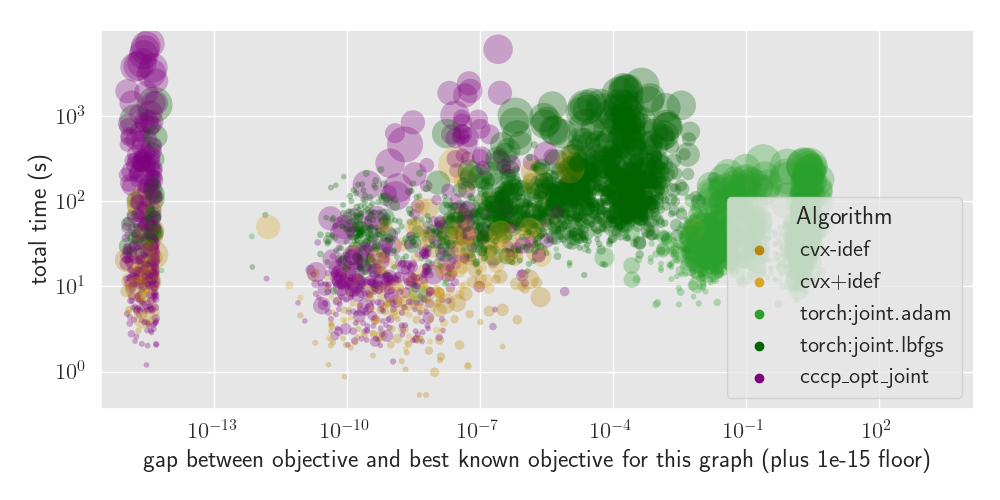
\includegraphics[width=0.67\linewidth]{figs/rand-joint/joint-gap-vs-time}%
    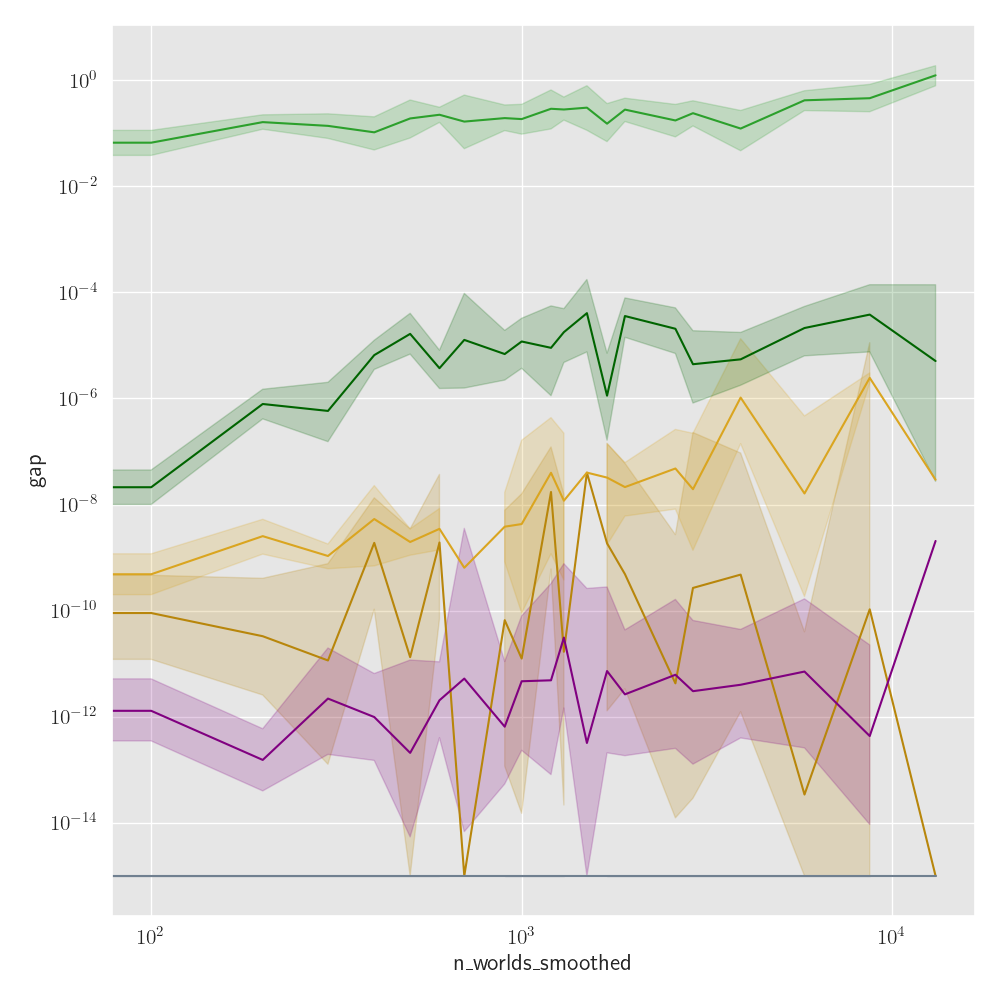
\includegraphics[width=0.32\linewidth]{figs/rand-joint/gap-vs-probsize-nolegend-big}
    \caption{
        % The resource costs: computation time (top) and maximum memory usage (bottom) for the various optimization methods (by color), as the size of the PDG increases.
        Accuracy and resource costs for the methods in \cref{sec:inf-as-cvx-program}.  
        Left: a scatter plot of several algorithms on random PDGs of $\approx 10$ variables. The $x$ axis is the score $\bbr{\dg M}_\gamma(\mu)$, where $\mu$ is the output of the algorithm (lower is better), and the $y$ axis is the time required to compute $\mu$. 
        Our methods are in gold $(0^+$-inference) and violet ($\zogamma$-inference); the baselines (black-box optimizers applied directly to \eqref{eqn:scoring-fn}) are in green.
        The area of each circle is proportional to the size of the optimization problem, as measured by
        % \verb|n_worlds|$\,=$
        $|\V\!\X|$.
        Right: the convex solvers maintain their edge in accuracy even as the problem grows.
     }\label{fig:joint-gap-time}
\end{figure*}

% \begin{linked}{lemma}{main}
%     % For   O( 3 n * ((3n+m+1)^3 ) * log(√n / ϵ) )  =   O( n^4 log(n)  log(1 / ϵ) )
% There is an algorithm that takes $O(n^4 \log n  \log \nf1\epsilon )$ time,
% and finds a point $\epsilon$-close in residual norm to the optimal distribution
% $\bbr{\dg M}^*$, where $n$ is the total number of parameters in a clique tree.
% \end{linked}

% Finally, we can do clique tree calibration as usual
% This gives yields a polynomial-time algorithm for marginal inference. If we are looking to answer a conditional probability query, $Q(Y|X{=}x)$,
% we can simply constrain the clique tree to satisfy $\mu_C(X{=}x)=1$ for all $C \in \cal C$ with $X \cap C \ne \emptyset$, and recalibrate the clique tree with standard methods
% % like belief propogation
% \parencite{koller2009probabilistic}, to get a clique tree representing the conditional distribution $\bbr{\dg M}^*|X{=}x$.
% Putting this all together, we get:

\begin{linked}{theorem}{main}
    %joe5*: what does "machine precision" mean here?
    %oli5: The entire approach is paramterized by an approximation accuracy \epsilon. The point of saying "machine precision" is just to say that we can fix \epsilon equal to a very small constant, say 1E-50, and then claim that we've computed the answer up to the the precision at which a computer represents numbers.
    % PDG inference can be solved to machine precision in 
%joe6*: Unless this terminology is completely standard and appears in
%lots of places, this must be explained.  Indeed, it should be
%exlained even if it appears in lots of places.  Have pity on the
%reader, who can't read your mind
    % Inference in a PDG can be done
    %oli6:
    % $\zogamma$-inference in a PDG can be 
    % Inference in a PDG 
    We can do
    PDG inference
    to precision 
    % $\nf1\epsilon$ in
    $\epsilon$ in 
    % to machine precision in
    % to precision $\nf1\epsilon$
    % $O( N^4 V^4 \log(N V) \exp(V T) )$ time, 
    \vspace{-0.8ex}
    \[ 
    % $
    % O\Big(  (N\!+\!A)^4 V^{4T} (\log (N\!+\!A) + T \log V ) \Big)
    O\pqty[\Big]{  (N\!+\!A)^4 V^{4T}
        \pqty[\Big]{ T \log V + \log \frac{N\!+\! A}{\epsilon} 
    %oli7: 
    % \cdot \frac{\max_a \beta_a}{\gamma \min_a \beta_a}
    % \cdot \frac{\max_a \beta_a}{\sigma}
    % \cdot 
    + \log
    \frac{\beta^{\max}}{\beta^{\min}}
        } }%
    % ~\text{where}
    \vspace{-1.5ex}
    \]
    time,
%joe9
%    \unskip\daggerfootnote{ at the cost of substantial overhead and
    \unskip\daggerfootnote{At the cost of substantial overhead and
    engineering effort, the exponent $4$ can be reduced to 2.872, by
      appeal to \textcite{nesterov1996infeasible} and the  
%joe7: You have to give a reference here, and say what the running
%time of the best multiplication algorithm is.  This is far too
%myhsterious. 
%oli7: done
    % current best matrix multiplication algorithm 
    current best matrix multiplication algorithm \parencite[$O(n^{2.372})$]{duan2022faster}
    to invert 
    %oli7: adding to clarify what $n$ is above:
    $n{\times} n$
    linear systems. }
    where:
    % ~~~\textbullet~
    % $\displaystyle \sigma = \begin{cases}
    %         {\gamma} & \text{ for $\zogamma$-inference } \\
    %         {\min_a \beta_a} & \text{ for $0^+\!$-inference }
    % \end{cases}$~,
    % $
    % time, where     
    \begin{itemize}[nosep,%
            % [label=$\blacktriangleright$
            ]
        \item $N$ is the total number of variables,
        \item $V$ is the number of values per variable,
        \item $T$ is the tree-width of the PDG's structure, 
        % and
        \item $A$ is the number of hyperarcs,
        %oli7: cleaning up this statement.
        % \item $\displaystyle\sigma \!=\! \frac{\min_a \beta_a}{\max_a \beta_a}$ 
        %     for $\gamma > 0$, and
        %     $\displaystyle\sigma \!=\! \frac{\gamma}{\max_a \beta_a}$ 
        %     for $0^+$.
            % $\frac{\gamma}{\max_a \beta_a}$ for $\zogamma$-inference.
        %
        % \item For $0^+$-inference, this bound holds if we erase $\gamma$; for $\gamma$-inference, it holds if we erase $\min_a \beta_a$.
        %
        % \item and
        % $\displaystyle \sigma = \begin{cases}
        %         \frac{\gamma}{\max_a \beta_a} & \text{ for $\zogamma$-inference } \\
        %         \frac{\min_a \beta_a}{\max_a \beta_a} & \text{ for $0^+\!$-inference }
        % \end{cases}$
        %
        \item $\beta^{\max}$ is the maximum observational confidence,
        and
        \item $\beta^{\min}$ is either $\gamma$ (for $\zogamma$-inference)
%joe9*: what is the "minimimum non-zero observational confidence"
          %Also, aren't there constraints on the \gamma's for which
          %this theorem holds?  If so, they should be stated clearly
          %in the theorem.         
          or the minimimum non-zero observational confidence (for
         $0^+$-inference). 
        % \item and 
        % $\displaystyle \sigma = \begin{cases}
        %         {\gamma} & \text{ for $\zogamma$-inference } \\
        %         {\min_a \beta_a} & \text{ for $0^+\!$-inference }
        % \end{cases}$.
    \end{itemize}
\end{linked}

% The proof rests almost entirely on the analysis of
% \textcite{badenbroek2021algorithm}
% % Badenbroek and Dahl (2021),
%  which certifies that the
% optimization algorithm detailed in
% % Dahl and Andersen (2022)
% \textcite{dahl2022primal}
% works in polynomial time.
% \otodo{REVIEW: the result \cref{prop:consistent-NP-hard} has nothing to do with tree width; a proper lower bound in this section ought to say we can't do better with bounded tree width, right? So is this the right place for it?}


% One might imagine that
% Thus, for  probabilistic queries may be answered in polynomial time
% Can we do any better?
% \textbf{Hardness.}
% We already know that PDG inference is NP
% Given a clique tree $\bmu$,
% A nautral question arises: is it any easier
% It seems obvious that the natural

% In a sense, computing $\bbr{\dg M}^*$ is a way of sorting through one's beleifs (the cpds of $\dg M$) and resolving all of the inconsistencies.
% Put anther way, we have computed the optimal
% More concretely
Our approach to inference computes
 % the inconsistency 
 $\aar{\dg M}_\gamma$ as a side effect of finding distributions of 
%joe4
%interest---but suppose we were only interested in calculating
%interest---but suppose we were only interested in calculating
interest.
%oli6:
% But suppose that we were interested in calculating only $\aar{\dg M}_\gamma$.
%joe7
%But suppose we were interested in calculating only this inconsistency.
But suppose that we were interested in calculating only this inconsistency.
% But suppose we were interested only in this inconsistency.
% Might we then have been able to ?
% Might we have been able to do so more cheaply,
Might there then be a more direct, asymptotically easier way 
%oli6:
% to calculate $\aar{\dg M}_\gamma$?
to do so?
% Or more simply put: is it any easier simply to notice whether there are inconsistencies present?
In general, the answer is no.

\begin{linked}{prop}{consistent-NP-hard}%\label{sharp-p-hard}
    \begin{enumerate}[nosep,label={\rm{(\alph*)}}]
    % \item Deciding if $\dg M$ is consistent is NP-ha{rd}.
    \item Deciding whether or not $\dg M$ is inconsistent is NP-hard.
    \item Computing $\aar{\dg M}_\gamma$ is \#P-hard, for all $\gamma \ge 0$.
    \end{enumerate}
\end{linked}

%joe4*: What about inference wrt [[M]], which is supposed to be what thue paper is about.
%oli4: actually all four things are approximately equivalent. I'll just use words
% In fact, calculating $\aar{\dg M}_\gamma$ and $\zogamma$-inference appear to be equally difficult;
%oli6: shortening.
% As we argue further in \cref{sec:inf-via-inc}, answering probablistic queries and calculating inconsistency are closely related problems, and appear to be equally difficult. 
% See \cref{sec:inf-via-inc} for further discussion on the deep relationship between these two problems.
% Rather, the two are deeply related
%oli8:
% The two problems are quite closely related; see \cref{sec:inf-via-inc}.
%joe9: It should say, if anything "In fact, the problems are
%intimaately related", but Appendix B should be cut.
%Rather, the problems are intimately related; see \cref{sec:inf-via-inc}.
% See \cref{sec:inf-via-inc} for further discussion.

% \begin{table}
%     % Let $m$ denote the
%     \centering
%     \begin{tabular}{ccc}
%         \toprule
%         & BP &  ExpCone \\\cmidrule(lr){2-3}
%         Time & $O(m t)$ & $O( m^4 \log m )$ \\
%         Memory  & $O(m + )$ {\color{red}??} & $O( m^2 )${\color{red}????}\\    \bottomrule
%     \end{tabular}
%
%     % \TODO[fill this in properly]
%
%     \caption{ }
% \end{table}
% \section{IMPLEMENTATION} \label{sec:implementation}
% \section{EMPIRICAL EVALUATION} \label{sec:expts}
\section{Experiments} \label{sec:expts}


Our experiments show that the techniques developed in \cref{sec:inf-as-cvx-program,sec:clique-tree-expcone} work significantly better than applying general-purpose optimization algorithms to \eqref{eqn:scoring-fn}.
%joe9
%In some ways it is surprising that $\bbr{\dg M}_\gamma$ poses any
%challege at all to standard optimization tools, given that it is
%infinitely differentiable in $\mu$, $\gamma$-strongly convex, and has
%derivatives  that have simple closed-form expressions.
It may seem surprising that $\bbr{\dg M}_\gamma$ poses a
challege to standard optimization tools, given that it is
infinitely differentiable in $\mu$, $\gamma$-strongly convex, and its
derivatives have simple closed-form expressions.
% Most of our experiments are synthetic.
%
% \cref{sec:inf-as-cvx-program} describes an optimization problem over 
%joe9
%But it does; we now illustrate this with
%synthetic experiments in two settings, 
%which correspond 
%to \cref{sec:inf-as-cvx-program,sec:clique-tree-expcone} respectively.
But it does, as we show with the following two synthetic experiments.

\textbf{Joint distribution optimization.} 
% We randomly generate small PDGs, and apply 
First, we randomly generate a small PDG $\dg M$.
%joe9
%Then, for
Then for 
$\gamma \in \{0, 0^+, 
    % 10^{-8}, 10^{-4},
     \ldots, \min_a \frac{\beta_a}{\alpha_a} \}$,
we optimize $\bbr{\dg M}_\gamma(\mu)$ over joint distributions $\mu$, 
%Joe9
%in one of several ways. 
%Either we use cvxpy \parencite{diamond2016cvxpy}
either by using cvxpy \parencite{diamond2016cvxpy}
to feed  
\eqref{prob:joint-inc}, \eqref{prob:joint-small-gamma}, or \eqref{prob:joint+idef} 
    to MOSEK \cite{mosek}, 
%joe9
%    or we use a standard optimizer (either Adam \parencite{kingma2014adam}
    or using a standard optimizer (either Adam \parencite{kingma2014adam}
    or LBFGS \parencite{fletcher2013practical}) built into
%joe9
%    \texttt{pytorch} \parencite{pytorch}, and choose a learning rate 
    \texttt{pytorch} \parencite{pytorch}, and choosing a learning rate 
    and a representation of $\mu$ in terms of optimization variables $\theta$. 
% Concretely, we use either $\mu \propto \max\{\theta, 0\}$ or $\mu \propto \exp(\theta)$. 
% These baselines are then run until convergence, or to a maximum of
    % 1500 iterations.
    %joe9
%We then iteratively optimize until convergence (or a time limit), and
We then iteratively optimize until convergence (or for a fixed time), and
    throw out the result if another choice of learning rate achieves a
smaller value of $\bbr{\dg M}_\gamma(\mu)$. 
% We then throw out all but the best learning rate.
The results are plotted in \cref{fig:joint-gap-time}.
Observe that our formulations (gold and violet) are significantly more accurate than the baselines, yet require similar amounts of time. In fact, the convex optimization is faster for small PDGs 
(although they do use more memory, and don't scale as well; see \cref{fig:resources} in \cref{sec:joint-expt-details}).
% However, they do require more memory, and the resource costs don't scale as well.
% values of $

\textbf{Clique tree optimization.} 
%joe9: I don't know what it means to adapt to Section 4
%We then adapt the procedure to \cref{sec:clique-tree-expcone} as follows:
We adapt the procedure to the techniques of
\cref{sec:clique-tree-expcone} as follows: 
%joe9
%first randomly generate a $k$-tree $T$ (a maximal graph of tree-width $k$),
first randomly generate a $k$-tree $T$ (a maximal graph of tree-width $k$)
and a PDG $\dg M$ whose hyperarcs lie within cliques of $T$; 
this ensures that the maximal cliques of $T$ form a tree-decomposition $(\C, \mathcal T)$ of $\dg M$'s structure.
%joe9
%Then, optimize $\bbr{\dg M}_\gamma(\Pr_{\!\bmu})$ over clique trees $\bmu$
Then optimize $\bbr{\dg M}_\gamma(\Pr_{\!\bmu})$ over clique trees $\bmu$
over $(\C, \mathcal T)$. 
%joe9: I didn't understand the next sentece.  What does it mean to
%encode the fact that they're not calibrated as constraints?  More
%generally, I didn't understand the whole approach.  Why does lack of
%calibration suggest that you add a loss term?
The issue is that such clique trees $\bmu$ may not be calibrated, which
we cannot directly encode as constraints. Instead, common practice is
to add a loss term.
%joe9
%Still, it is sometimes advantages for the optimizer to simply pay the
Still, it is sometimes advantageous for the optimizer to simply pay the
price to violate the constraint, which allows an optimizer to
``cheat'' by returning marginals that cannot be achieved by any joint
distribution.
%joe9: I really couldn't follow what was going on here.  I think
%you're trying to deal with the problems you found, but I'm not sure
%that the typical reader will be able to follow this.
Thus, before we evaluate, we must first recalibrate the clique tree \parencite[\S10]{koller2009probabilistic}.
Because of these additional challenges, the baselines do less well in this setting.
See \cref{fig:} in \cref{sec:clus-expt-details}.
% We defer the figures and tables to the appendix.

\textbf{Evaluation on BNs.}
%joe9: similar to what?
We find that very similar results for small BNs.
However, belief propogation is much faster and at least as accurate,
    in those cases where it applies.
% For PDGs that are also BNs or FGs, belief propogation is strictly faster.  
% Details for all experiments, as well as tables, and more figures can
    % be found in \cref{sec:expt-setup}.
    %joe9
    %More figures and details about all experiments may be found in
    More figures and details about all experiments can be found in
\cref{sec:expt-setup}. 
%joe7*: We need to say more here.  It took decades to get these better
%algorithms for BNs.  Ours is a first step.  We should that we expect
%that comparable improvements are possible!
% It took decades


\section{Discussion}

% We have provided an implementation of PDG inference and proved that is correct and fixed-parameter tractable. 
We have defined a family of inference notions for PDGs, 
given a fixed-parameter tractable algorithm for it, and shown that it 
out-performs our baselines.
% \begin{enumerate}
%     \item \end{enumerate}

Still, much remains to be said about inference in PDGs. 
% Asymptotically, there may be much for improvement.
Our implementation runs in time $\tilde O(N^4)$, and our analysis suggests one of time $\tilde O(N^{2.872})$. 
But under bounded tree-width, inference in other graphical models, and nearly all graph problems can be solved in $O(N^1)$ time. Can we do better?
%joe8: added: we need something like this.
%oli8: thanks.  Just added the word "long" below
Given the long history of improvements 
%oli8: too many prepositions; forming a noun phrase:
% for algorithms for inference in Bayesian networks,
to Bayesian network inference algorithms,
we are optimistic that we can.

 %joe7*: don't undercut your result!
%joe9
%More importantly, we have only shown how to do inference in a small
More importantly, we have shown how to do inference only in a 
subset of cases: 
 %joe8: why "cleanly"
%oli8: removed; I agree it's better without.  I wrote it that way because our techniques do work in a slightly broader set of circumstances (e.g., via the CCCP, as in the last pagaraph.)
%oli8: this is inefficient
when the $\zogamma$-semantics is a 
%joe8: moreover and moreover and moreover
%oli8: Yeah... I found it humerous and I liked how it emphasized how narrow the conditions are that this works. But in retrospect it is not a good idea to emphasize that too much in the conclusion. And generally, you're probably right that this style of humor does't belong in the paper (maybe in a talk). 
% singleton, and moreover $\bbr{\dg M}_{\gamma}$ is convex, and moreover, and
%joe9: i'm having rouble following this.  If observatinoal dominance
%implies convexity, why bother mentioning convexity?
%singleton, because $\bbr{\dg M}_{\gamma}$ is convex, 
%and in addition convexity comes from a point-wise ``observational
singleton, and either $\bbeta \ge \gamma \balpha$ or $\bbeta \gg
\balpha$.  
%oli8:
% The other cases are certainly of interest as well.
Other cases are certainly of interest as well.
% The general case is certainly also of interest.
When $\bbeta = 0$ and $(\Ar, \balpha)$ represents independencies of a Bayesian Network, for instance, PDG inference amounts to \emph{qualitative} inference in a BN, i.e., describing the BN's independecies. 
% Another problem of interest that can be written as PDG inference is
% Some optimal transport problems can also be written as questions about PDG inference; to give just the idea, note that $\bbr{ p(X) , q(Y)}_0^*$ is the set of couplings between $p(X)$ and $q(Y)$. 
% A much more difficult problem than the one we solved, would be to find an approach that addresses all of these instance of inference in PDGs.
%joe8: we have no idea how difficult it is
%oli8: we have some idea. None of the three of us have any idea how 
%A much more difficult problem than the one we solved, would be to find
% It would be of interest to find an approach that addresses all of these instance of inference in PDGs. 
%joe7
%While, our analysis doesn't quite address any of these problems, it
%oli7
% While our analysis doesn't address these problems, it
%joe9*: Cut this and the corresponding appendix.  Saying that we have
%a bunch of ideas that don't work is not helpful, and takes up room.
\discard{
Our analysis does not resove these problems, but it
    does shed light on some of them.  
% there are two other cases that our analyses a small amount of light on.
The $0$-semantics, for instance, is 
%oli8: removing
% essentially
characterized by \cref{prop:marginonly,prop:cluster-inc-correct}, 
% even though we haven't said anything about how to answer queries with respect to this set.
%oli8: lots of edits; didn't think my old version was worth saving so they're not tracked.
Also, when $\bbr{\dg M}_\gamma$ is not convex, we can still find an optimal distribution with the concave-convex procedure \cite{yuille2003concave}, which we do in \cref{sec:larger-gamma}---but this only suffices for inference if we already know there's a unique optimal distribution.
}
% Doing inference in these general cases appears to be more difficult, and is still very much an open problem.
\discard{
In some cases, this might actually allow us to do inference---say, if we happen to know for external reasons that $\bbr{\dg M}^*_\gamma$ is pseudo-convex (although we loose polynomial time guarantees and have no ability to automatically recognize such situations). In any case, we have implemented this, and describe it in \cref{sec:larger-gamma}.}
%joe7*: this is an awfully weak way to end the paper
%oli7*: agreed!
%oli8*: ... what to say at the end, though? Try something like this...
%joe9
%We are curious if it is possible to address all of these instance of
%PDG inference with a uniform approach. 
We are currently working on extending our results so that they apply
more broadly.